\documentclass[makeidx,envcountchap,graybox,deutsch,ngerman,sectrefs]{svmono}
%\documentclass[envcountchap,graybox,deutsch,sectrefs]{svmono}
%%%%% eigene tempor�re Abk�rzungsliste, f�r die Zeit, bis einheitliche Schreibungen bestehen
\usepackage{tempshort}
%%  Von Springer empfohlene Pakete %% 
%%\documentclass[envcountsect,graybox,deutsch,sectrefs]{svmono}
\usepackage{chapterbib}
\usepackage{type1cm}
\usepackage[ansinew]{inputenc}
\usepackage{babel}
\usepackage[pdftex]{graphicx} %PDF-Vektorgrafiken einbinden
\usepackage{newtxtext} %Typischer Springer-Font
\usepackage{newtxmath}
\usepackage{multicol}
\usepackage[bottom]{footmisc} %Platziert alle Fu�noten unten  
\usepackage[nobreak]{cite}
%\usepackage{biblatex}
\usepackage{cancel}
\usepackage[absolute]{textpos}
\usepackage{graphicx}
\usepackage{pdfpages}

%\usepackage{floatrow}
%\usepackage{mwe}
\usepackage[figuresright]{rotating}
\usepackage{bigints}
\let\laplace\relax  % Vermeidung der Fehlermeldung "\laplace already defined."
\usepackage{trfsigns}
\usepackage{amsmath}
\usepackage{tabulary}
\usepackage{tabularx}

%%  Eigene Pakete %%
\usepackage{adjustbox}
\usepackage{wasysym}
\usepackage{gensymb}
\usepackage{float}
\usepackage{caption}
\usepackage[left=5cm,right=4cm,top=3cm,bottom=4cm,includeheadfoot]{geometry}

%\usepackage{wasysym}
%\usepackage{bigints}
%\usepackage{esint}
%\usepackage{relsize,exscale}

\usepackage{mathtools}   % Vermeidung der Fehlermeldung "Undefined control sequence \coloneqq."


% header and footer
\usepackage{fancyhdr}
\pagestyle{fancy}
\fancyhead[LE,RO]\thepage
\renewcommand{\sectionmark}[1]{\markright{\thesection.\ #1}}
%\fancyhead[LO]{\nouppercase\leftmark}
%\fancyhead[RE]{\nouppercase\rightmark}
\fancyhead[LO]{\nouppercase\rightmark}
\fancyhead[RE]{\nouppercase\leftmark}
\fancyfoot{}
% svmono hat offenbar irgendwas merkw�rdig definiert, darum mu� hier verbreitert werden
%\addtolength\headwidth{25pt}
\setlength{\headheight}{25pt}

%% Units
\usepackage{siunitx}
\sisetup{
  locale = US,
  per-mode = reciprocal, %symbol, % | reciprocal | fraction | ?
  exponent-product = \cdot,
  separate-uncertainty,
  %exponent-to-prefix,
  %prefixes-as-symbols = false,
  %list-units = brackets,% | single | repeat
  %range-units = brackets,% | single | repeat
  %multi-part-units = brackets,% | single | repeat
}
\usepackage{chngcntr}
\usepackage{booktabs}
\usepackage{slashed}
\usepackage{listings}
\usepackage{color} %red, green, blue, yellow, cyan, magenta, black, white
%\usepackage{color} %Einfache Farbendefinition -> von Graybox-Option ben�tigt
\usepackage{multirow}
\usepackage{longtable} %Tabellen �ber mehrere Seiten hinweg
\usepackage{framed} % von Graybox-Option ben�tigt
\usepackage[shortlabels]{enumitem} %Erweiterte Aufz�hloptionen
\usepackage{array}
\usepackage[xindy]{imakeidx} %Wortindex und Personenindex erstellen

\usepackage[hyphens]{url}
%\usepackage[breaklinks,colorlinks=true,linkcolor=black,urlcolor=blue,citecolor=black,filecolor=green,hyperfootnotes=false]{hyperref}
\usepackage[                                    %Hyperref erstellt ein Bookmark/Lesezeichen im PDF. siehe https://www.namsu.de/Extra/pakete/Hyperref.html
bookmarksopen=true,															%Das Lesezeichen ist ge�ffnet beim �ffnen der PDF.
bookmarksnumbered=true,                         %Zahlen werden im Bookmark angezeigt.   
plainpages=false,
pdfpagelabels,
colorlinks=true,                                %Links werden farbig dargestellt.
linkcolor=black, citecolor=black, urlcolor=cyan %Farben definieren.
]{hyperref}                                     %Sollte als letztes eingebunden werden, da es sehr viele Verweise und �nderungen erzeugt. Das Packet ist sehr stark, aber auch umfangreich ist. 

%\usepackage[breaklinks,colorlinks=true,linkcolor=black,urlcolor=blue,citecolor=black,filecolor=green,hyperfootnotes=false]{hyperref}
%\usepackage[breaklinks,colorlinks=true,linkcolor=black,urlcolor=blue,citecolor=black,filecolor=green,hyperfootnotes=false
            %pdftex,
            %pdfauthor={Kaschke, Cartarius},
            %pdftitle={Finger�bungen der Physik}
            %pdfsubject={Ein Repetitorium und �bungsbuch zu im Studium wenig behandelten Kapiteln der Physik mit ausf�hrlich behandelten Problemen und MATLAB-Programmen},
            %pdfkeywords={Physik, Mechanik}
            %]{hyperref}
\pdfminorversion=5

\usepackage{hypcap}
\usepackage[record,section=section,stylemods={mcols},automake]{glossaries-extra}
\usepackage{glossary-longextra}
%\usepackage{glossary-bookindex}
%\makeindex
\setglossarystyle{long-name-sym-desc-loc}
\setabbreviationstyle[acronym]{long-short}

\definecolor{killA}{rgb}{.7,.3,.3}
\newcommand\killA[1]{\bgroup\color{killA}{\cancel{#1}}\egroup}
\newcommand\killB[1]{\bgroup\color{cyan!30!black}{\cancel{#1}}\egroup}

% typographisch korrekte Abk�rzungen (needs to be loaded after hyperref)
\usepackage{abbrev}
\newglossary*{bew}{Glossar}
\newglossary*{hm}{Glossar}
\newglossary*{adyn}{Glossar}
\newglossary*{kontmech}{Glossar}
\newglossary*{aero}{Glossar}
\newglossary*{edyn}{Glossar}
\newglossary*{spo}{Glossar}
\newglossary*{optbas}{Glossar}
\newglossary*{optger}{Glossar}
\newglossary*{optatm}{Glossar}
\newglossary*{optspez}{Glossar}
\GlsXtrLoadResources[src={bew/gloss},type=bew]
\GlsXtrLoadResources[src={hm/gloss},type=hm]
\GlsXtrLoadResources[src={adyn/gloss},type=adyn]
\GlsXtrLoadResources[src={kontmech/gloss},type=kontmech]
\GlsXtrLoadResources[src={aero/gloss},type=aero]
\GlsXtrLoadResources[src={spo/gloss},type=spo]
\GlsXtrLoadResources[src={edyn/gloss},type=edyn]
\GlsXtrLoadResources[src={optbas/gloss},type=optbas]
\GlsXtrLoadResources[src={optger/gloss},type=optger]
\GlsXtrLoadResources[src={optatm/gloss},type=optatm]
\GlsXtrLoadResources[src={optspez/gloss},type=optspez]
\glssetcategoryattribute{bew}{indexname}{true}
%\renewcommand\index\newterm
%\newcolumntype{g}[1]{>{\RaggedRight\hspace{0pt}}p{#1}}
%\renewcommand\glslongextraNameAlign{g}
\renewcommand\glslongextraLocationAlign{@{\ ~\ }>{\raggedright}p{\glspagelistwidth}}
\definecolor{gls}{rgb}{.4,.4,.5}
\renewcommand*{\glstextformat}[1]{\textcolor{gls}{#1}}

%Absatzregeln
\clubpenalty = 30000 %Keine einzelnen Absatzzeilen
\widowpenalty = 30000
\setlength{\parindent}{0em} 
\newcolumntype{L}[1]{>{\raggedright\arraybackslash}p{#1}}
\newcolumntype{C}[1]{>{\centering\arraybackslash}p{#1}}
\newcolumntype{R}[1]{>{\raggedleft\arraybackslash}p{#1}}

\usepackage{xstring}

\newcommand\mfile[2]{%
\saveexpandmode\noexpandarg
\StrSubstitute{#2}{_}{\_}[\tmpname]
\restoreexpandmode
\href{MatlabDateien/\chapname/#1\tmpname}{\tmpname}}

%%% Hyperlinks zu MATLAB Dateien
%\newcommand\mlref[1]{\mfile{}{#1}}
%\newcommand\mlinclref[1]{\mfile{IncludeFolder/}{#1}}
%\newcommand\mldataref[1]{\mfile{Data/}{#1}}

%%% .. f�r ein Verzeichnis hoch
%%% . f�r aktuelle Verzeichnis
%% lokal: MatlabDateien/bew
%\newcommand\mlbewref[1]{\href{MatlabDateien/bew/#1}{#1}}
%% git: https://github.com/sn-code-inside/fingeruebungen-physik/tree/main/bew

\newcommand{\mlrefwithindex}[2]{%
  \index[mfiles]{#2}%   <-- Eintrag im M-File-Index mit aktueller Seitenzahl
  \href{https://github.com/sn-code-inside/fingeruebungen-physik/tree/main/#1/#2}{#2}%
}


%\newcommand\mlbewref[1]{\href{https://github.com/sn-code-inside/fingeruebungen-physik/tree/main/bew/#1}{#1}}
%\newcommand\mlbewdref[1]{\href{https://github.com/sn-code-inside/fingeruebungen-physik/tree/main/bew/Data/#1}{#1}}
%\newcommand\mlbewiref[1]{\href{https://github.com/sn-code-inside/fingeruebungen-physik/tree/main/bew/IncludeFolder/#1}{#1}}
%\newcommand\mlkontmechref[1]{\href{https://github.com/sn-code-inside/fingeruebungen-physik/tree/main/kontmech/#1}{#1}}
%\newcommand\mlkontmechdref[1]{\href{https://github.com/sn-code-inside/fingeruebungen-physik/tree/main/kontmech/Data/#1}{#1}}
%\newcommand\mlkontmechiref[1]{\href{https://github.com/sn-code-inside/fingeruebungen-physik/tree/main/kontmech/IncludeFolder/#1}{#1}}
%\newcommand\mlhmref[1]{\href{https://github.com/sn-code-inside/fingeruebungen-physik/tree/main/hm/#1}{#1}}
%\newcommand\mlhmdref[1]{\href{https://github.com/sn-code-inside/fingeruebungen-physik/tree/main/hm/Data/#1}{#1}}
%\newcommand\mlhmiref[1]{\href{https://github.com/sn-code-inside/fingeruebungen-physik/tree/main/hm/IncludeFolder/#1}{#1}}
%\newcommand\mladynref[1]{\href{https://github.com/sn-code-inside/fingeruebungen-physik/tree/main/adyn/#1}{#1}}
%\newcommand\mladyndref[1]{\href{https://github.com/sn-code-inside/fingeruebungen-physik/tree/main/adyn/Data/#1}{#1}}
%\newcommand\mladyniref[1]{\href{https://github.com/sn-code-inside/fingeruebungen-physik/tree/main/adyn/IncludeFolder/#1}{#1}}
%\newcommand\mledynref[1]{\href{https://github.com/sn-code-inside/fingeruebungen-physik/tree/main/edyn/#1}{#1}}
%\newcommand\mledyndref[1]{\href{https://github.com/sn-code-inside/fingeruebungen-physik/tree/main/edyn/Data/#1}{#1}}
%\newcommand\mledyniref[1]{\href{https://github.com/sn-code-inside/fingeruebungen-physik/tree/main/edyn/IncludeFolder/#1}{#1}}
%\newcommand\mloptbasref[1]{\href{https://github.com/sn-code-inside/fingeruebungen-physik/tree/main/optbas/#1}{#1}}
%\newcommand\mloptbasdref[1]{\href{https://github.com/sn-code-inside/fingeruebungen-physik/tree/main/optbas/Data/#1}{#1}}
%\newcommand\mloptbasiref[1]{\href{https://github.com/sn-code-inside/fingeruebungen-physik/tree/main/optbas/IncludeFolder/#1}{#1}}
%\newcommand\mloptspezref[1]{\href{https://github.com/sn-code-inside/fingeruebungen-physik/tree/main/optspez/#1}{#1}}
%\newcommand\mloptspezdref[1]{\href{https://github.com/sn-code-inside/fingeruebungen-physik/tree/main/optspez/Data/#1}{#1}}
%\newcommand\mloptspeziref[1]{\href{https://github.com/sn-code-inside/fingeruebungen-physik/tree/main/optspez/IncludeFolder/#1}{#1}}

\newcommand\mlbewref[1]{\mlrefwithindex{bew}{#1}}
\newcommand\mlbewdref[1]{\mlrefwithindex{bew/Data}{#1}}
\newcommand\mlbewiref[1]{\mlrefwithindex{bew/Include}{#1}}
\newcommand\mlkontmechref[1]{\mlrefwithindex{kontmech}{#1}}
\newcommand\mlkontmechdref[1]{\mlrefwithindex{kontmech/Data}{#1}}
\newcommand\mlkontmechiref[1]{\mlrefwithindex{kontmech/Include}{#1}}
\newcommand\mlhmref[1]{\mlrefwithindex{hm}{#1}}
\newcommand\mlhmdref[1]{\mlrefwithindex{hm/Data}{#1}}
\newcommand\mlhmiref[1]{\mlrefwithindex{hm/Include}{#1}}
\newcommand\mladynref[1]{\mlrefwithindex{adyn}{#1}}
\newcommand\mladyndref[1]{\mlrefwithindex{adyn/Data}{#1}}
\newcommand\mladyniref[1]{\mlrefwithindex{adyn/Index}{#1}}
\newcommand\mledynref[1]{\mlrefwithindex{edyn}{#1}}
\newcommand\mledyndref[1]{\mlrefwithindex{edyn/Data}{#1}}
\newcommand\mledyniref[1]{\mlrefwithindex{edyn/Index}{#1}}
\newcommand\mloptbasref[1]{\mlrefwithindex{optbas}{#1}}
\newcommand\mloptbasdref[1]{\mlrefwithindex{optbas/Data}{#1}}
\newcommand\mloptbasiref[1]{\mlrefwithindex{optbas/Include}{#1}}
\newcommand\mloptspezref[1]{\mlrefwithindex{optspez}{#1}}
\newcommand\mloptspezdref[1]{\mlrefwithindex{optspez/Data}{#1}}
\newcommand\mloptspeziref[1]{\mlrefwithindex{optspez/Include}{#1}}
\newcommand\mloptgerref[1]{\mlrefwithindex{optger}{#1}}
\newcommand\mloptgerdref[1]{\mlrefwithindex{optger/Data}{#1}}
\newcommand\mloptgeriref[1]{\mlrefwithindex{optger/Include}{#1}}
\newcommand\mloptatmref[1]{\mlrefwithindex{optatm}{#1}}
\newcommand\mloptatmdref[1]{\mlrefwithindex{optatm/Data}{#1}}
\newcommand\mloptatmiref[1]{\mlrefwithindex{optatm/Include}{#1}}



\newcommand\mlcmd[1]{\textcolor{cyan}{\texttt{#1}}}

%Grafikregeln
\graphicspath{{hm/graphs/}
	                    	{bew/graphs/}
     						{kontmech/graphs/}
							{hm/graphs/}
							{adyn/graphs/}
							{edyn/graphs/}
							{kontmech/graphs/}
							{spo/graphs/}
							{optbas/graphs/}
							{optger/graphs/}
							{optatm/graphs/}
							{solman/graphs/}
                                                        {aero/graphs}}
\DeclareGraphicsExtensions{.pdf, .png, .jpg, .jpeg}
\def\figname{Abb}
\newcommand\figref[1]{\figname.\ \ref{abb:#1}}
\usepackage[labelfont=bf]{caption}

\usepackage{tocloft}
\usepackage{etoc}
\setlength\cftfignumwidth{30pt}

% Flatterrand links
\cftsetindents{chapter}{0em}{4em}
\cftsetindents{section}{1.5em}{4em}
\cftsetindents{subsection}{3.8em}{4em}

% flacher Rand links
%\cftsetindents{chapter}{0em}{4em}
%\cftsetindents{section}{0em}{4em}
%\cftsetindents{subsection}{0em}{4em}

\newcommand\partitle[1]{
\addcontentsline{toc}{part}{#1}
\begin{titlepage}
  %\vskip 60%\p@
  \begin{center}
    {\LARGE Finger�bungen der Physik -- #1 \par}
    \vskip 3em%
    {\large Michael Kaschke und Holger Cartarius\par}
  \end{center}
\end{titlepage}
}

%\newcommand\mlref[1]{\href{\chapname/matlab/#1}{#1}}
%\newcommand\mlinclref[1]{\href{\chapname/matlab/IncludeFolder/#1}{\color{cyan}{#1}}}

%Neue Kommandos
\newcommand{\lk}{\left(}        %gro�e runde Klammer (links)
\newcommand{\rk}{\right )}      %gro�e runde Klammer (rechts)
\newcommand{\lgk}{\left \{}     %gro�e geschweifte Klammer (links)
\newcommand{\rgk}{\right \}}    %gro�e geschweifte Klammer (rechts)
\newcommand{\lek}{\left [}      %gro�e eckige Klammer (links)
\newcommand{\rek}{\right ]}     %gro�e eckige Klammer (rechts)
\newcommand{\anf}[1]{\glqq#1\grqq}    %Deutsche Anf�hrungszeichen: \anf{}
\newcommand{\defined}{:=}				%Definition
\newcommand{\curl}{\text{\textbf{rot}}\,}	%Rotation-Operator curl()
\newcommand{\ket}[1]{|#1\rangle}		%Quantenmechanischer Zustand
\newcommand{\curvelintri}{\,\overset{\blacktriangle}{\smallfrown}}
\newcommand{\straighttri}{\blacktriangle}
\newcommand{\UT}{\text{UT}}
\newcommand{\UTC}{\text{UTC}}
\newcommand{\JD}{\text{JD}}
\newcommand{\JDE}{\text{JDE}}
\newcommand{\MJD}{\text{MJD}}
\newcommand{\TDT}{\text{TDT}}
\newcommand{\TT}{\text{TT}}
\newcommand{\NVS}{\text{Navier-Stokes-Gleichungen}}
\newcommand{\MWG}{\text{Maxwell-Gleichungen}}
\newcommand{\EMW}{\text{Elektromagnetische Wellen}}
\newcommand{\eMW}{\text{elektromagnetischen Wellen}}
\newcommand{\RT}{\text{Relativit�tstheorie~}}
\newcommand{\au}{\mathrm{AE}}
\newcommand{\ET}{\text{ET}}
\newcommand{\TAI}{\text{TAI}}
\newcommand{\GMST}{\text{GMST}}
\newcommand{\LMST}{\text{LMST}}
\newcommand{\MESZ}{\text{MESZ}}
\newcommand{\KOS}{\text{Koordinatensystem }}
\newcommand{\DGL}{\text{Differentialgleichung }}
\newcommand{\NA}{\text{NA}}
\newcommand{\uA}{\text{u}}  %atomare Masseneinheit
\newcommand{\MOZ}{\text{MOZ}}
\newcommand{\grad}{\text{\textbf{grad}}\,}	%Gradient-Operator grad()
\newcommand{\uproman}[1]{\mathrm{\uppercase\expandafter{\romannumeral#1}}}
\newcommand{\lowroman}[1]{\romannumeral#1\relax}

\newcommand\todo[1]{\textcolor{red}{TODO: #1}}

\renewcommand{\=}[1]{\stackrel{\text{#1}}{=}}  %Schrift �ber Gleich-Zeichen
\renewcommand{\d}{\partial}
\newcommand{\lra}{\Leftrightarrow}  %�quivalenz-Pfeile
\newcommand{\abs}[1]{\left\vert#1\right\vert}     %Betragsklammern
\renewcommand{\Re}{\mathrm{Re}}                          %Realteil
\renewcommand{\Im}{\mathrm{Im}}                          %Imagin�rteil
\renewcommand{\im}{\mathrm{i}}                         %Imagin�re Einheit
\renewcommand{\epsilon}{\varepsilon} 
\newcommand{\keff}{k_\text{eff}}
\newcommand{\con}{\text{const}}
\newcommand{\conv}{\vec{const}}
\newcommand{\PL}{\mathcal{P}_}
\newcommand{\artanh}{\mathrm{artanh}}
% QED-Symbol im text- bzw. Mathemodus
\newcommand{\textqed}{\hfill ~ $\square$}
\newcommand{\mmqed}{\tag*{$\square$}}

\newcommand{\fa}{(\textbf{a}) }
\newcommand{\fb}{(\textbf{b}) }
\newcommand{\fc}{(\textbf{c}) }
\newcommand{\fd}{(\textbf{d}) }
\newcommand{\fe}{(\textbf{e}) }
\newcommand{\ff}{(\textbf{f}) }

\newcommand{\iF}{im Folgenden~}
\newcommand{\iA}{im Allgemeinen~}


\DeclareMathOperator\divv{div}
\DeclareMathOperator\res{Res}
\DeclareMathOperator{\sech}{sech}
\DeclareMathOperator\sgn{sgn}

% f�r Appendix - MATLAB Referenz
\newcommand{\rotv}{\vec{rot}\,}
\newcommand{\gradv}{\vec{grad}\,}
\newcommand{\nablav}{\vec{\nabla}\,}

\newcommand{\ceil}{\mathrm{ceil}}
\newcommand{\sinc}{\mathrm{sinc}}
\newcommand{\diag}{\mathrm{diag}}
\newcommand{\sign}{\mathrm{sign}}
\newcommand{\length}{\mathrm{length}}
\newcommand{\sort}{\mathrm{sort}}
\newcommand{\summ}{\mathrm{sum}}
\newcommand{\asin}{\mathrm{asin}}
\newcommand{\acos}{\mathrm{acos}}
\newcommand{\atan}{\mathrm{atan}}
\newcommand{\prodd}{\mathrm{prod}}
\newcommand{\median}{\mathrm{mediab}}
\newcommand{\mean}{\mathrm{mean}}
\newcommand{\std}{\mathrm{std}}
\newcommand{\eye}{\mathrm{eye}}
\newcommand{\zeros}{\mathrm{zeros}}
\newcommand{\ones}{\mathrm{ones}}
\newcommand{\rand}{\mathrm{rand}}
\newcommand{\inline}{\mathrm{inline}}
\newcommand{\modd}{\mathrm{mod}}
\newcommand{\floor}{\mathrm{floor}}
\newcommand{\round}{\mathrm{round}}
\newcommand{\rem}{\mathrm{rem}}
\newcommand{\sqrtt}{\mathrm{sqrt}}
\newcommand{\triu}{\mathrm{triu}}
\newcommand{\tril}{\mathrm{tril}}
\newcommand{\size}{\mathrm{size}}
\newcommand{\dett}{\mathrm{det}}
\newcommand{\inv}{\mathrm{inv}}
\newcommand{\rank}{\mathrm{rank}}
\newcommand{\rref}{\mathrm{rref}}
\newcommand{\eig}{\mathrm{eig}}
\newcommand{\poly}{\mathrm{poly}}
\newcommand{\lu}{\mathrm{lu}}
\newcommand{\qr}{\mathrm{qr}}
\newcommand{\quaddd}{\mathrm{quad}}
\newcommand{\fzero}{\mathrm{fzero}}
\newcommand{\roots}{\mathrm{roots}}
\newcommand{\odezd}{\textcolor{mygreen}{\texttt{ode23}}}
\newcommand{\odevf}{\textcolor{mygreen}{\texttt{ode45}}}
\newcommand{\odeeds}{\textcolor{mygreen}{\texttt{ode13s}}}
\newcommand{\odeefs}{\textcolor{mygreen}{\texttt{ode15s}}}
\newcommand{\ddezd}{\textcolor{mygreen}{\texttt{dde23}}}
\newcommand{\onlineZ}{online verf�gbaren Zusatzmaterialien{}}
\newcommand{\MKc}{\url{https://www.fingeruebungen-physik.de}{}}
\newcommand{\linklsg}{\href{https://www.fingeruebungen-physik.de}{\textcolor{blue} {$\rightarrow$ L�sungsteil.}}}
\newcommand{\githubSN}{\url{https://github.com/sn-code-inside/fingeruebungen-physik}{}\,\,}

\newcommand{\FT}{\mathcal{F}} %Fourier-Transformierte

% Aufz�hlung der L�sungen der Teilaufgaben
\newlist{subprobs}{enumerate}{1}
\setlist[subprobs]{
  label= \textbf{\textit{Teilaufgabe}} \textbf{\textit{\arabic*:}} \protect\thissubprob,
  ref=\arabic*, itemsep=\baselineskip, align=left}
\newcommand{\subprob}[1]{
  \def\thissubprob{\textbf{\textit{#1}}}\item ~\vspace{0.2\baselineskip} \newline}

\renewenvironment{example}[1]{
\refstepcounter{example}\par\medskip
\begin{shaded} 
\begin{samepage}
\noindent \textbf{\textit{Beispiel~\theexample: {#1}}}\\ 
\noindent{\color{black} \rule{\textwidth}{0.2 mm}}
\end{samepage}
}{\end{shaded}
\noindent{\color{black} \rule{\textwidth}{0.2 mm}}
} % or snugshade
\definecolor{shadecolor}{gray}{0.95}
\definecolor{mygreen}{RGB}{28,172,0} % color values Red, Green, Blue
\definecolor{mylilas}{RGB}{170,55,241}

\newenvironment{infobox}[1]{
     \begin{shaded} 
     \begin{samepage}
\noindent{\color{black} \rule{\textwidth}{0.2 mm}}
     \end{samepage}
}{\end{shaded}
\noindent{\color{black} \rule{\textwidth}{0.2 mm}}
} 
\definecolor{shadecolor}{gray}{0.95}
\definecolor{mygreen}{RGB}{28,172,0} % color values Red, Green, Blue
\definecolor{mylilas}{RGB}{170,55,241}


\newenvironment{nebenrechnung}[1]{
\begin{shaded} 
\begin{samepage}
\noindent\textbf{Nebenrechnung: \\} 
\noindent{\color{black} \rule{0.1\columnwidth}{0.2mm} \\}
\end{samepage}
}{\end{shaded}
\noindent{\color{black} \rule{0.1\columnwidth}{0.2mm} \\}
} % or snugshade
\definecolor{shadecolor}{gray}{0.95}
\definecolor{mygreen}{RGB}{28,172,0} % color values Red, Green, Blue
\definecolor{mylilas}{RGB}{170,55,241}

\newenvironment{merksatz}[1]{
\begin{shaded} 
\begin{samepage}
\noindent\textbf{Merke:\\} 
\noindent{\color{black} \rule{0.9\columnwidth}{0.2mm} \\ \\}
\end{samepage}
}{\end{shaded}
\noindent{\color{black} \rule{0.9\columnwidth}{0.2mm} \\}
} % or snugshade


\lstset{language=Matlab,%
    %basicstyle=\color{red},
    %basicstyle={\linespread{0.9}\ttfamily},
    basicstyle=\footnotesize\ttfamily,
    breaklines=true,%
    morekeywords={matlab2tikz},
    keywordstyle={\small \color{mygreen}},%
    morekeywords=[2]{1}, keywordstyle=[2]{\small\color{black}},
    identifierstyle={\small \color{black}},%
    stringstyle={\small\color{mylilas}},
    commentstyle={\small\color{mylilas}},%
    showstringspaces=false,%without this there will be a symbol in the places where there is a space
    numbers=left,%
    numberstyle={\tiny \color{black}},% size of the numbers
    numbersep=9pt, % this defines how far the numbers are from the text
    emph=[1]{for,end,else,break, function},emphstyle=[1]\small \color{blue}, %some words to emphasise
    emph=[2]{odeset},emphstyle=[2]\small \color{mygreen}, %some words to emphasise
    %emph=[2]{word1,word2}, emphstyle=[2]{style},    
}

%\bibliographystyle{spphys.bst}

%Trennregeln f�r spezielle Worte
%\hyphenation{Fresnel \matlab �qui-nok-ti-um}

\DeclareSIUnit\erg{erg}
\DeclareSIUnit\cal{cal}
\DeclareSIUnit\celsius{C}
\DeclareSIUnit\m{M}
\DeclareSIUnit\kel{K^{-4}}

%Stichwort- und Personenverzeichnis
\makeindex[title=Stichwortverzeichnis] % Create the default index
\makeindex[name=personen,title=Personenverzeichnis] % Create an index named 'personen'
\newcommand{\indexp}[1]{\index[personen]{#1}}
\makeindex[name=mfiles,title=MATLAB-Skriptverzeichnis,columns=2]

% list of exercises
\newcommand{\loxname}{\Large �bungsverzeichnis}  % einheitliche Gr��e Large
\newlistof[chapter]{prob}{lox}\loxname
\newcommand\uebung[3][]{\label{prob:#2}%
\addcontentsline{lox}{prob}{\protect\numberline{}{\probRef{#2}:~#3#1}}%
\textbf{#1#3}\\[\baselineskip]}
\makeatletter
\renewcommand{\l@prob}{\@dottedtocline{1}{0em}{0em}}
\makeatother

\newcommand\einfach{\uebung[~$\ast$~~]}
\newcommand\mittel{\uebung[~$\ast\,\ast$~~]}
\newcommand\schwierig{\uebung[~$\ast\,\ast\,\ast$~~]}
\newcommand\zusatz{\uebung[~$\ast\,\ast\,\ast\,!$~~]}
%\newcommand\einfach{\uebung[~\textbf{*}~~]}
%\newcommand\mittel{\uebung[~\textbf{*\,*}~~]}
%\newcommand\schwierig{\uebung[~\textbf{*\,*\,*}~]}
%\newcommand\zusatz{\uebung[~\textbf{*\,*\,*\,!}~~]}
\usepackage[atend]{bookmark}
%\BookmarkAtEnd{%
%\bookmarksetup{startatroot}\bookmark[level=0,named=\loxname]{}}

\newcommand\kapitel[1]{Kapitel \ref{kap:#1}}
%\newcommand\kap[1]{Kap.\ \ref{kap:#1}}
\newcommand\kap[1]{Kap. \ref{kap:#1}}

\begin{document}
% customize prob and sol in svmono
\makeatletter
%\counterwithin*{chapter}{part}

\spn@wtheorem{prob}{\bgroup\exercisename\egroup}{\bfseries}{\rmfamily}
\makeatother
\renewenvironment{sol}[1]{\par\addvspace{6pt}\noindent\phantomsection{\textbf{L�sung \ref{#1}}} \ignorespaces}{\par\addvspace{6pt}}
\newcommand\probRef[1]{�bung \ref{prob:#1}}
\renewcommand\probref[1]{\textbf{\probRef{#1}}}
\newcommand\lsgref[1]{L�sung \ref{lsg:#1}}

\newcommand\sbullet[1][.5]{\mathbin{\vcenter{\hbox{\scalebox{#1}{$\bullet$}}}}}

\setcounter{table}{0}



\author{Michael Kaschke, Holger Cartarius und Ulrich Potthoff}
\title{Finger�bungen der Physik \\ \\ 
\medskip
\matlab{} -- Anhang}

%\subtitle{Zusatzmaterial zum Repetitorium und �bungsbuch zu im Studium wenig behandelten Kapiteln der Physik mit ausf�hrlich behandelten Problemen und \matlab-Programmen \\ \\
%Unter Mitwirkung von Ulrich Potthoff}
\smallskip
\maketitle

\frontmatter%%%%%%%%%%%%%%%%%%%%%%%%%%%%%%%%%%%%%%%%%%%>

\newpage 

\tableofcontents
\newcounter{fmpg}\setcounter{fmpg}{\arabic{page}}

\mainmatter

%%%%%%%%%%%%%%%%%%%%%%%%%%%%%%%%%%%%%%%%%%%%%%%%
%\part*{MATLAB\\ \medskip Teil I Mechanik} \label{chap:matlab}
%\addcontentsline{toc}{part}{MATLAB} 
%\addcontentsline{toc}{part}{MATLAB-Skripte}

\makeatletter
\@addtoreset{chapter}{part}
\makeatother
\renewcommand{\thechapter}{M\,\arabic{chapter}}
\setcounter{chapter}{0}

%\begin{bibunit}[spphys]

%\documentclass[makeidx,envcountchap,graybox,deutsch,ngerman,sectrefs]{svmono}
%\documentclass[envcountchap,graybox,deutsch,sectrefs]{svmono}
%%%%% eigene tempor�re Abk�rzungsliste, f�r die Zeit, bis einheitliche Schreibungen bestehen
\usepackage{tempshort}
%%  Von Springer empfohlene Pakete %% 
%%\documentclass[envcountsect,graybox,deutsch,sectrefs]{svmono}
\usepackage{chapterbib}
\usepackage{type1cm}
\usepackage[ansinew]{inputenc}
\usepackage{babel}
\usepackage[pdftex]{graphicx} %PDF-Vektorgrafiken einbinden
\usepackage{newtxtext} %Typischer Springer-Font
\usepackage{newtxmath}
\usepackage{multicol}
\usepackage[bottom]{footmisc} %Platziert alle Fu�noten unten  
\usepackage[nobreak]{cite}
%\usepackage{biblatex}
\usepackage{cancel}
\usepackage[absolute]{textpos}
\usepackage{graphicx}
\usepackage{pdfpages}

%\usepackage{floatrow}
%\usepackage{mwe}
\usepackage[figuresright]{rotating}
\usepackage{bigints}
\let\laplace\relax  % Vermeidung der Fehlermeldung "\laplace already defined."
\usepackage{trfsigns}
\usepackage{amsmath}
\usepackage{tabulary}
\usepackage{tabularx}

%%  Eigene Pakete %%
\usepackage{adjustbox}
\usepackage{wasysym}
\usepackage{gensymb}
\usepackage{float}
\usepackage{caption}
\usepackage[left=5cm,right=4cm,top=3cm,bottom=4cm,includeheadfoot]{geometry}

%\usepackage{wasysym}
%\usepackage{bigints}
%\usepackage{esint}
%\usepackage{relsize,exscale}

\usepackage{mathtools}   % Vermeidung der Fehlermeldung "Undefined control sequence \coloneqq."


% header and footer
\usepackage{fancyhdr}
\pagestyle{fancy}
\fancyhead[LE,RO]\thepage
\renewcommand{\sectionmark}[1]{\markright{\thesection.\ #1}}
%\fancyhead[LO]{\nouppercase\leftmark}
%\fancyhead[RE]{\nouppercase\rightmark}
\fancyhead[LO]{\nouppercase\rightmark}
\fancyhead[RE]{\nouppercase\leftmark}
\fancyfoot{}
% svmono hat offenbar irgendwas merkw�rdig definiert, darum mu� hier verbreitert werden
%\addtolength\headwidth{25pt}
\setlength{\headheight}{25pt}

%% Units
\usepackage{siunitx}
\sisetup{
  locale = US,
  per-mode = reciprocal, %symbol, % | reciprocal | fraction | ?
  exponent-product = \cdot,
  separate-uncertainty,
  %exponent-to-prefix,
  %prefixes-as-symbols = false,
  %list-units = brackets,% | single | repeat
  %range-units = brackets,% | single | repeat
  %multi-part-units = brackets,% | single | repeat
}
\usepackage{chngcntr}
\usepackage{booktabs}
\usepackage{slashed}
\usepackage{listings}
\usepackage{color} %red, green, blue, yellow, cyan, magenta, black, white
%\usepackage{color} %Einfache Farbendefinition -> von Graybox-Option ben�tigt
\usepackage{multirow}
\usepackage{longtable} %Tabellen �ber mehrere Seiten hinweg
\usepackage{framed} % von Graybox-Option ben�tigt
\usepackage[shortlabels]{enumitem} %Erweiterte Aufz�hloptionen
\usepackage{array}
\usepackage[xindy]{imakeidx} %Wortindex und Personenindex erstellen

\usepackage[hyphens]{url}
%\usepackage[breaklinks,colorlinks=true,linkcolor=black,urlcolor=blue,citecolor=black,filecolor=green,hyperfootnotes=false]{hyperref}
\usepackage[                                    %Hyperref erstellt ein Bookmark/Lesezeichen im PDF. siehe https://www.namsu.de/Extra/pakete/Hyperref.html
bookmarksopen=true,															%Das Lesezeichen ist ge�ffnet beim �ffnen der PDF.
bookmarksnumbered=true,                         %Zahlen werden im Bookmark angezeigt.   
plainpages=false,
pdfpagelabels,
colorlinks=true,                                %Links werden farbig dargestellt.
linkcolor=black, citecolor=black, urlcolor=cyan %Farben definieren.
]{hyperref}                                     %Sollte als letztes eingebunden werden, da es sehr viele Verweise und �nderungen erzeugt. Das Packet ist sehr stark, aber auch umfangreich ist. 

%\usepackage[breaklinks,colorlinks=true,linkcolor=black,urlcolor=blue,citecolor=black,filecolor=green,hyperfootnotes=false]{hyperref}
%\usepackage[breaklinks,colorlinks=true,linkcolor=black,urlcolor=blue,citecolor=black,filecolor=green,hyperfootnotes=false
            %pdftex,
            %pdfauthor={Kaschke, Cartarius},
            %pdftitle={Finger�bungen der Physik}
            %pdfsubject={Ein Repetitorium und �bungsbuch zu im Studium wenig behandelten Kapiteln der Physik mit ausf�hrlich behandelten Problemen und MATLAB-Programmen},
            %pdfkeywords={Physik, Mechanik}
            %]{hyperref}
\pdfminorversion=5

\usepackage{hypcap}
\usepackage[record,section=section,stylemods={mcols},automake]{glossaries-extra}
\usepackage{glossary-longextra}
%\usepackage{glossary-bookindex}
%\makeindex
\setglossarystyle{long-name-sym-desc-loc}
\setabbreviationstyle[acronym]{long-short}

\definecolor{killA}{rgb}{.7,.3,.3}
\newcommand\killA[1]{\bgroup\color{killA}{\cancel{#1}}\egroup}
\newcommand\killB[1]{\bgroup\color{cyan!30!black}{\cancel{#1}}\egroup}

% typographisch korrekte Abk�rzungen (needs to be loaded after hyperref)
\usepackage{abbrev}
\newglossary*{bew}{Glossar}
\newglossary*{hm}{Glossar}
\newglossary*{adyn}{Glossar}
\newglossary*{kontmech}{Glossar}
\newglossary*{aero}{Glossar}
\newglossary*{edyn}{Glossar}
\newglossary*{spo}{Glossar}
\newglossary*{optbas}{Glossar}
\newglossary*{optger}{Glossar}
\newglossary*{optatm}{Glossar}
\newglossary*{optspez}{Glossar}
\GlsXtrLoadResources[src={bew/gloss},type=bew]
\GlsXtrLoadResources[src={hm/gloss},type=hm]
\GlsXtrLoadResources[src={adyn/gloss},type=adyn]
\GlsXtrLoadResources[src={kontmech/gloss},type=kontmech]
\GlsXtrLoadResources[src={aero/gloss},type=aero]
\GlsXtrLoadResources[src={spo/gloss},type=spo]
\GlsXtrLoadResources[src={edyn/gloss},type=edyn]
\GlsXtrLoadResources[src={optbas/gloss},type=optbas]
\GlsXtrLoadResources[src={optger/gloss},type=optger]
\GlsXtrLoadResources[src={optatm/gloss},type=optatm]
\GlsXtrLoadResources[src={optspez/gloss},type=optspez]
\glssetcategoryattribute{bew}{indexname}{true}
%\renewcommand\index\newterm
%\newcolumntype{g}[1]{>{\RaggedRight\hspace{0pt}}p{#1}}
%\renewcommand\glslongextraNameAlign{g}
\renewcommand\glslongextraLocationAlign{@{\ ~\ }>{\raggedright}p{\glspagelistwidth}}
\definecolor{gls}{rgb}{.4,.4,.5}
\renewcommand*{\glstextformat}[1]{\textcolor{gls}{#1}}

%Absatzregeln
\clubpenalty = 30000 %Keine einzelnen Absatzzeilen
\widowpenalty = 30000
\setlength{\parindent}{0em} 
\newcolumntype{L}[1]{>{\raggedright\arraybackslash}p{#1}}
\newcolumntype{C}[1]{>{\centering\arraybackslash}p{#1}}
\newcolumntype{R}[1]{>{\raggedleft\arraybackslash}p{#1}}

\usepackage{xstring}

\newcommand\mfile[2]{%
\saveexpandmode\noexpandarg
\StrSubstitute{#2}{_}{\_}[\tmpname]
\restoreexpandmode
\href{MatlabDateien/\chapname/#1\tmpname}{\tmpname}}

%%% Hyperlinks zu MATLAB Dateien
%\newcommand\mlref[1]{\mfile{}{#1}}
%\newcommand\mlinclref[1]{\mfile{IncludeFolder/}{#1}}
%\newcommand\mldataref[1]{\mfile{Data/}{#1}}

%%% .. f�r ein Verzeichnis hoch
%%% . f�r aktuelle Verzeichnis
%% lokal: MatlabDateien/bew
%\newcommand\mlbewref[1]{\href{MatlabDateien/bew/#1}{#1}}
%% git: https://github.com/sn-code-inside/fingeruebungen-physik/tree/main/bew

\newcommand{\mlrefwithindex}[2]{%
  \index[mfiles]{#2}%   <-- Eintrag im M-File-Index mit aktueller Seitenzahl
  \href{https://github.com/sn-code-inside/fingeruebungen-physik/tree/main/#1/#2}{#2}%
}


%\newcommand\mlbewref[1]{\href{https://github.com/sn-code-inside/fingeruebungen-physik/tree/main/bew/#1}{#1}}
%\newcommand\mlbewdref[1]{\href{https://github.com/sn-code-inside/fingeruebungen-physik/tree/main/bew/Data/#1}{#1}}
%\newcommand\mlbewiref[1]{\href{https://github.com/sn-code-inside/fingeruebungen-physik/tree/main/bew/IncludeFolder/#1}{#1}}
%\newcommand\mlkontmechref[1]{\href{https://github.com/sn-code-inside/fingeruebungen-physik/tree/main/kontmech/#1}{#1}}
%\newcommand\mlkontmechdref[1]{\href{https://github.com/sn-code-inside/fingeruebungen-physik/tree/main/kontmech/Data/#1}{#1}}
%\newcommand\mlkontmechiref[1]{\href{https://github.com/sn-code-inside/fingeruebungen-physik/tree/main/kontmech/IncludeFolder/#1}{#1}}
%\newcommand\mlhmref[1]{\href{https://github.com/sn-code-inside/fingeruebungen-physik/tree/main/hm/#1}{#1}}
%\newcommand\mlhmdref[1]{\href{https://github.com/sn-code-inside/fingeruebungen-physik/tree/main/hm/Data/#1}{#1}}
%\newcommand\mlhmiref[1]{\href{https://github.com/sn-code-inside/fingeruebungen-physik/tree/main/hm/IncludeFolder/#1}{#1}}
%\newcommand\mladynref[1]{\href{https://github.com/sn-code-inside/fingeruebungen-physik/tree/main/adyn/#1}{#1}}
%\newcommand\mladyndref[1]{\href{https://github.com/sn-code-inside/fingeruebungen-physik/tree/main/adyn/Data/#1}{#1}}
%\newcommand\mladyniref[1]{\href{https://github.com/sn-code-inside/fingeruebungen-physik/tree/main/adyn/IncludeFolder/#1}{#1}}
%\newcommand\mledynref[1]{\href{https://github.com/sn-code-inside/fingeruebungen-physik/tree/main/edyn/#1}{#1}}
%\newcommand\mledyndref[1]{\href{https://github.com/sn-code-inside/fingeruebungen-physik/tree/main/edyn/Data/#1}{#1}}
%\newcommand\mledyniref[1]{\href{https://github.com/sn-code-inside/fingeruebungen-physik/tree/main/edyn/IncludeFolder/#1}{#1}}
%\newcommand\mloptbasref[1]{\href{https://github.com/sn-code-inside/fingeruebungen-physik/tree/main/optbas/#1}{#1}}
%\newcommand\mloptbasdref[1]{\href{https://github.com/sn-code-inside/fingeruebungen-physik/tree/main/optbas/Data/#1}{#1}}
%\newcommand\mloptbasiref[1]{\href{https://github.com/sn-code-inside/fingeruebungen-physik/tree/main/optbas/IncludeFolder/#1}{#1}}
%\newcommand\mloptspezref[1]{\href{https://github.com/sn-code-inside/fingeruebungen-physik/tree/main/optspez/#1}{#1}}
%\newcommand\mloptspezdref[1]{\href{https://github.com/sn-code-inside/fingeruebungen-physik/tree/main/optspez/Data/#1}{#1}}
%\newcommand\mloptspeziref[1]{\href{https://github.com/sn-code-inside/fingeruebungen-physik/tree/main/optspez/IncludeFolder/#1}{#1}}

\newcommand\mlbewref[1]{\mlrefwithindex{bew}{#1}}
\newcommand\mlbewdref[1]{\mlrefwithindex{bew/Data}{#1}}
\newcommand\mlbewiref[1]{\mlrefwithindex{bew/Include}{#1}}
\newcommand\mlkontmechref[1]{\mlrefwithindex{kontmech}{#1}}
\newcommand\mlkontmechdref[1]{\mlrefwithindex{kontmech/Data}{#1}}
\newcommand\mlkontmechiref[1]{\mlrefwithindex{kontmech/Include}{#1}}
\newcommand\mlhmref[1]{\mlrefwithindex{hm}{#1}}
\newcommand\mlhmdref[1]{\mlrefwithindex{hm/Data}{#1}}
\newcommand\mlhmiref[1]{\mlrefwithindex{hm/Include}{#1}}
\newcommand\mladynref[1]{\mlrefwithindex{adyn}{#1}}
\newcommand\mladyndref[1]{\mlrefwithindex{adyn/Data}{#1}}
\newcommand\mladyniref[1]{\mlrefwithindex{adyn/Index}{#1}}
\newcommand\mledynref[1]{\mlrefwithindex{edyn}{#1}}
\newcommand\mledyndref[1]{\mlrefwithindex{edyn/Data}{#1}}
\newcommand\mledyniref[1]{\mlrefwithindex{edyn/Index}{#1}}
\newcommand\mloptbasref[1]{\mlrefwithindex{optbas}{#1}}
\newcommand\mloptbasdref[1]{\mlrefwithindex{optbas/Data}{#1}}
\newcommand\mloptbasiref[1]{\mlrefwithindex{optbas/Include}{#1}}
\newcommand\mloptspezref[1]{\mlrefwithindex{optspez}{#1}}
\newcommand\mloptspezdref[1]{\mlrefwithindex{optspez/Data}{#1}}
\newcommand\mloptspeziref[1]{\mlrefwithindex{optspez/Include}{#1}}
\newcommand\mloptgerref[1]{\mlrefwithindex{optger}{#1}}
\newcommand\mloptgerdref[1]{\mlrefwithindex{optger/Data}{#1}}
\newcommand\mloptgeriref[1]{\mlrefwithindex{optger/Include}{#1}}
\newcommand\mloptatmref[1]{\mlrefwithindex{optatm}{#1}}
\newcommand\mloptatmdref[1]{\mlrefwithindex{optatm/Data}{#1}}
\newcommand\mloptatmiref[1]{\mlrefwithindex{optatm/Include}{#1}}



\newcommand\mlcmd[1]{\textcolor{cyan}{\texttt{#1}}}

%Grafikregeln
\graphicspath{{hm/graphs/}
	                    	{bew/graphs/}
     						{kontmech/graphs/}
							{hm/graphs/}
							{adyn/graphs/}
							{edyn/graphs/}
							{kontmech/graphs/}
							{spo/graphs/}
							{optbas/graphs/}
							{optger/graphs/}
							{optatm/graphs/}
							{solman/graphs/}
                                                        {aero/graphs}}
\DeclareGraphicsExtensions{.pdf, .png, .jpg, .jpeg}
\def\figname{Abb}
\newcommand\figref[1]{\figname.\ \ref{abb:#1}}
\usepackage[labelfont=bf]{caption}

\usepackage{tocloft}
\usepackage{etoc}
\setlength\cftfignumwidth{30pt}

% Flatterrand links
\cftsetindents{chapter}{0em}{4em}
\cftsetindents{section}{1.5em}{4em}
\cftsetindents{subsection}{3.8em}{4em}

% flacher Rand links
%\cftsetindents{chapter}{0em}{4em}
%\cftsetindents{section}{0em}{4em}
%\cftsetindents{subsection}{0em}{4em}

\newcommand\partitle[1]{
\addcontentsline{toc}{part}{#1}
\begin{titlepage}
  %\vskip 60%\p@
  \begin{center}
    {\LARGE Finger�bungen der Physik -- #1 \par}
    \vskip 3em%
    {\large Michael Kaschke und Holger Cartarius\par}
  \end{center}
\end{titlepage}
}

%\newcommand\mlref[1]{\href{\chapname/matlab/#1}{#1}}
%\newcommand\mlinclref[1]{\href{\chapname/matlab/IncludeFolder/#1}{\color{cyan}{#1}}}

%Neue Kommandos
\newcommand{\lk}{\left(}        %gro�e runde Klammer (links)
\newcommand{\rk}{\right )}      %gro�e runde Klammer (rechts)
\newcommand{\lgk}{\left \{}     %gro�e geschweifte Klammer (links)
\newcommand{\rgk}{\right \}}    %gro�e geschweifte Klammer (rechts)
\newcommand{\lek}{\left [}      %gro�e eckige Klammer (links)
\newcommand{\rek}{\right ]}     %gro�e eckige Klammer (rechts)
\newcommand{\anf}[1]{\glqq#1\grqq}    %Deutsche Anf�hrungszeichen: \anf{}
\newcommand{\defined}{:=}				%Definition
\newcommand{\curl}{\text{\textbf{rot}}\,}	%Rotation-Operator curl()
\newcommand{\ket}[1]{|#1\rangle}		%Quantenmechanischer Zustand
\newcommand{\curvelintri}{\,\overset{\blacktriangle}{\smallfrown}}
\newcommand{\straighttri}{\blacktriangle}
\newcommand{\UT}{\text{UT}}
\newcommand{\UTC}{\text{UTC}}
\newcommand{\JD}{\text{JD}}
\newcommand{\JDE}{\text{JDE}}
\newcommand{\MJD}{\text{MJD}}
\newcommand{\TDT}{\text{TDT}}
\newcommand{\TT}{\text{TT}}
\newcommand{\NVS}{\text{Navier-Stokes-Gleichungen}}
\newcommand{\MWG}{\text{Maxwell-Gleichungen}}
\newcommand{\EMW}{\text{Elektromagnetische Wellen}}
\newcommand{\eMW}{\text{elektromagnetischen Wellen}}
\newcommand{\RT}{\text{Relativit�tstheorie~}}
\newcommand{\au}{\mathrm{AE}}
\newcommand{\ET}{\text{ET}}
\newcommand{\TAI}{\text{TAI}}
\newcommand{\GMST}{\text{GMST}}
\newcommand{\LMST}{\text{LMST}}
\newcommand{\MESZ}{\text{MESZ}}
\newcommand{\KOS}{\text{Koordinatensystem }}
\newcommand{\DGL}{\text{Differentialgleichung }}
\newcommand{\NA}{\text{NA}}
\newcommand{\uA}{\text{u}}  %atomare Masseneinheit
\newcommand{\MOZ}{\text{MOZ}}
\newcommand{\grad}{\text{\textbf{grad}}\,}	%Gradient-Operator grad()
\newcommand{\uproman}[1]{\mathrm{\uppercase\expandafter{\romannumeral#1}}}
\newcommand{\lowroman}[1]{\romannumeral#1\relax}

\newcommand\todo[1]{\textcolor{red}{TODO: #1}}

\renewcommand{\=}[1]{\stackrel{\text{#1}}{=}}  %Schrift �ber Gleich-Zeichen
\renewcommand{\d}{\partial}
\newcommand{\lra}{\Leftrightarrow}  %�quivalenz-Pfeile
\newcommand{\abs}[1]{\left\vert#1\right\vert}     %Betragsklammern
\renewcommand{\Re}{\mathrm{Re}}                          %Realteil
\renewcommand{\Im}{\mathrm{Im}}                          %Imagin�rteil
\renewcommand{\im}{\mathrm{i}}                         %Imagin�re Einheit
\renewcommand{\epsilon}{\varepsilon} 
\newcommand{\keff}{k_\text{eff}}
\newcommand{\con}{\text{const}}
\newcommand{\conv}{\vec{const}}
\newcommand{\PL}{\mathcal{P}_}
\newcommand{\artanh}{\mathrm{artanh}}
% QED-Symbol im text- bzw. Mathemodus
\newcommand{\textqed}{\hfill ~ $\square$}
\newcommand{\mmqed}{\tag*{$\square$}}

\newcommand{\fa}{(\textbf{a}) }
\newcommand{\fb}{(\textbf{b}) }
\newcommand{\fc}{(\textbf{c}) }
\newcommand{\fd}{(\textbf{d}) }
\newcommand{\fe}{(\textbf{e}) }
\newcommand{\ff}{(\textbf{f}) }

\newcommand{\iF}{im Folgenden~}
\newcommand{\iA}{im Allgemeinen~}


\DeclareMathOperator\divv{div}
\DeclareMathOperator\res{Res}
\DeclareMathOperator{\sech}{sech}
\DeclareMathOperator\sgn{sgn}

% f�r Appendix - MATLAB Referenz
\newcommand{\rotv}{\vec{rot}\,}
\newcommand{\gradv}{\vec{grad}\,}
\newcommand{\nablav}{\vec{\nabla}\,}

\newcommand{\ceil}{\mathrm{ceil}}
\newcommand{\sinc}{\mathrm{sinc}}
\newcommand{\diag}{\mathrm{diag}}
\newcommand{\sign}{\mathrm{sign}}
\newcommand{\length}{\mathrm{length}}
\newcommand{\sort}{\mathrm{sort}}
\newcommand{\summ}{\mathrm{sum}}
\newcommand{\asin}{\mathrm{asin}}
\newcommand{\acos}{\mathrm{acos}}
\newcommand{\atan}{\mathrm{atan}}
\newcommand{\prodd}{\mathrm{prod}}
\newcommand{\median}{\mathrm{mediab}}
\newcommand{\mean}{\mathrm{mean}}
\newcommand{\std}{\mathrm{std}}
\newcommand{\eye}{\mathrm{eye}}
\newcommand{\zeros}{\mathrm{zeros}}
\newcommand{\ones}{\mathrm{ones}}
\newcommand{\rand}{\mathrm{rand}}
\newcommand{\inline}{\mathrm{inline}}
\newcommand{\modd}{\mathrm{mod}}
\newcommand{\floor}{\mathrm{floor}}
\newcommand{\round}{\mathrm{round}}
\newcommand{\rem}{\mathrm{rem}}
\newcommand{\sqrtt}{\mathrm{sqrt}}
\newcommand{\triu}{\mathrm{triu}}
\newcommand{\tril}{\mathrm{tril}}
\newcommand{\size}{\mathrm{size}}
\newcommand{\dett}{\mathrm{det}}
\newcommand{\inv}{\mathrm{inv}}
\newcommand{\rank}{\mathrm{rank}}
\newcommand{\rref}{\mathrm{rref}}
\newcommand{\eig}{\mathrm{eig}}
\newcommand{\poly}{\mathrm{poly}}
\newcommand{\lu}{\mathrm{lu}}
\newcommand{\qr}{\mathrm{qr}}
\newcommand{\quaddd}{\mathrm{quad}}
\newcommand{\fzero}{\mathrm{fzero}}
\newcommand{\roots}{\mathrm{roots}}
\newcommand{\odezd}{\textcolor{mygreen}{\texttt{ode23}}}
\newcommand{\odevf}{\textcolor{mygreen}{\texttt{ode45}}}
\newcommand{\odeeds}{\textcolor{mygreen}{\texttt{ode13s}}}
\newcommand{\odeefs}{\textcolor{mygreen}{\texttt{ode15s}}}
\newcommand{\ddezd}{\textcolor{mygreen}{\texttt{dde23}}}
\newcommand{\onlineZ}{online verf�gbaren Zusatzmaterialien{}}
\newcommand{\MKc}{\url{https://www.fingeruebungen-physik.de}{}}
\newcommand{\linklsg}{\href{https://www.fingeruebungen-physik.de}{\textcolor{blue} {$\rightarrow$ L�sungsteil.}}}
\newcommand{\githubSN}{\url{https://github.com/sn-code-inside/fingeruebungen-physik}{}\,\,}

\newcommand{\FT}{\mathcal{F}} %Fourier-Transformierte

% Aufz�hlung der L�sungen der Teilaufgaben
\newlist{subprobs}{enumerate}{1}
\setlist[subprobs]{
  label= \textbf{\textit{Teilaufgabe}} \textbf{\textit{\arabic*:}} \protect\thissubprob,
  ref=\arabic*, itemsep=\baselineskip, align=left}
\newcommand{\subprob}[1]{
  \def\thissubprob{\textbf{\textit{#1}}}\item ~\vspace{0.2\baselineskip} \newline}

\renewenvironment{example}[1]{
\refstepcounter{example}\par\medskip
\begin{shaded} 
\begin{samepage}
\noindent \textbf{\textit{Beispiel~\theexample: {#1}}}\\ 
\noindent{\color{black} \rule{\textwidth}{0.2 mm}}
\end{samepage}
}{\end{shaded}
\noindent{\color{black} \rule{\textwidth}{0.2 mm}}
} % or snugshade
\definecolor{shadecolor}{gray}{0.95}
\definecolor{mygreen}{RGB}{28,172,0} % color values Red, Green, Blue
\definecolor{mylilas}{RGB}{170,55,241}

\newenvironment{infobox}[1]{
     \begin{shaded} 
     \begin{samepage}
\noindent{\color{black} \rule{\textwidth}{0.2 mm}}
     \end{samepage}
}{\end{shaded}
\noindent{\color{black} \rule{\textwidth}{0.2 mm}}
} 
\definecolor{shadecolor}{gray}{0.95}
\definecolor{mygreen}{RGB}{28,172,0} % color values Red, Green, Blue
\definecolor{mylilas}{RGB}{170,55,241}


\newenvironment{nebenrechnung}[1]{
\begin{shaded} 
\begin{samepage}
\noindent\textbf{Nebenrechnung: \\} 
\noindent{\color{black} \rule{0.1\columnwidth}{0.2mm} \\}
\end{samepage}
}{\end{shaded}
\noindent{\color{black} \rule{0.1\columnwidth}{0.2mm} \\}
} % or snugshade
\definecolor{shadecolor}{gray}{0.95}
\definecolor{mygreen}{RGB}{28,172,0} % color values Red, Green, Blue
\definecolor{mylilas}{RGB}{170,55,241}

\newenvironment{merksatz}[1]{
\begin{shaded} 
\begin{samepage}
\noindent\textbf{Merke:\\} 
\noindent{\color{black} \rule{0.9\columnwidth}{0.2mm} \\ \\}
\end{samepage}
}{\end{shaded}
\noindent{\color{black} \rule{0.9\columnwidth}{0.2mm} \\}
} % or snugshade


\lstset{language=Matlab,%
    %basicstyle=\color{red},
    %basicstyle={\linespread{0.9}\ttfamily},
    basicstyle=\footnotesize\ttfamily,
    breaklines=true,%
    morekeywords={matlab2tikz},
    keywordstyle={\small \color{mygreen}},%
    morekeywords=[2]{1}, keywordstyle=[2]{\small\color{black}},
    identifierstyle={\small \color{black}},%
    stringstyle={\small\color{mylilas}},
    commentstyle={\small\color{mylilas}},%
    showstringspaces=false,%without this there will be a symbol in the places where there is a space
    numbers=left,%
    numberstyle={\tiny \color{black}},% size of the numbers
    numbersep=9pt, % this defines how far the numbers are from the text
    emph=[1]{for,end,else,break, function},emphstyle=[1]\small \color{blue}, %some words to emphasise
    emph=[2]{odeset},emphstyle=[2]\small \color{mygreen}, %some words to emphasise
    %emph=[2]{word1,word2}, emphstyle=[2]{style},    
}

%\bibliographystyle{spphys.bst}

%Trennregeln f�r spezielle Worte
%\hyphenation{Fresnel \matlab �qui-nok-ti-um}

\DeclareSIUnit\erg{erg}
\DeclareSIUnit\cal{cal}
\DeclareSIUnit\celsius{C}
\DeclareSIUnit\m{M}
\DeclareSIUnit\kel{K^{-4}}

%Stichwort- und Personenverzeichnis
\makeindex[title=Stichwortverzeichnis] % Create the default index
\makeindex[name=personen,title=Personenverzeichnis] % Create an index named 'personen'
\newcommand{\indexp}[1]{\index[personen]{#1}}
\makeindex[name=mfiles,title=MATLAB-Skriptverzeichnis,columns=2]

% list of exercises
\newcommand{\loxname}{\Large �bungsverzeichnis}  % einheitliche Gr��e Large
\newlistof[chapter]{prob}{lox}\loxname
\newcommand\uebung[3][]{\label{prob:#2}%
\addcontentsline{lox}{prob}{\protect\numberline{}{\probRef{#2}:~#3#1}}%
\textbf{#1#3}\\[\baselineskip]}
\makeatletter
\renewcommand{\l@prob}{\@dottedtocline{1}{0em}{0em}}
\makeatother

\newcommand\einfach{\uebung[~$\ast$~~]}
\newcommand\mittel{\uebung[~$\ast\,\ast$~~]}
\newcommand\schwierig{\uebung[~$\ast\,\ast\,\ast$~~]}
\newcommand\zusatz{\uebung[~$\ast\,\ast\,\ast\,!$~~]}
%\newcommand\einfach{\uebung[~\textbf{*}~~]}
%\newcommand\mittel{\uebung[~\textbf{*\,*}~~]}
%\newcommand\schwierig{\uebung[~\textbf{*\,*\,*}~]}
%\newcommand\zusatz{\uebung[~\textbf{*\,*\,*\,!}~~]}
\usepackage[atend]{bookmark}
%\BookmarkAtEnd{%
%\bookmarksetup{startatroot}\bookmark[level=0,named=\loxname]{}}

\newcommand\kapitel[1]{Kapitel \ref{kap:#1}}
%\newcommand\kap[1]{Kap.\ \ref{kap:#1}}
\newcommand\kap[1]{Kap. \ref{kap:#1}}

\begin{document}
% customize prob and sol in svmono
\makeatletter
%\counterwithin*{chapter}{part}

\spn@wtheorem{prob}{\bgroup\exercisename\egroup}{\bfseries}{\rmfamily}
\makeatother
\renewenvironment{sol}[1]{\par\addvspace{6pt}\noindent\phantomsection{\textbf{L�sung \ref{#1}}} \ignorespaces}{\par\addvspace{6pt}}
\newcommand\probRef[1]{�bung \ref{prob:#1}}
\renewcommand\probref[1]{\textbf{\probRef{#1}}}
\newcommand\lsgref[1]{L�sung \ref{lsg:#1}}

\newcommand\sbullet[1][.5]{\mathbin{\vcenter{\hbox{\scalebox{#1}{$\bullet$}}}}}

\setcounter{table}{0}


%%%%%%%%%%%%%%%%%%%%%%%%%%%%%%%%%%%%%%%%%%%%%%%%%%%%%%%%%%%%%

\chapter{\matlab-Basics} \label{kap:solman_matlab}

Im Folgenden sollen einige \matlab-Elemente und -Funktionalit�ten vorgestellt werden. Es geht hierbei nicht darum, eine Vorlesungsskript oder gar ein kurzgefasstes Lehrbuch f�r \matlab{} zusammenzustellen. Dazu gibt es viele hervorragende Standardwerke (\zb \cite{Wilson2003, Pietruszka2020, Schweizer2016, Attaway2013}) und auch umfangreiche Online-Dokumentationen im Internet (\zb \url{https://www.mathworks.com/matlabcentral}). Wir wollen mit der Zusammenstellung die Themen herausheben, die in der Computational Physics (CP) h�ufig vorkommen.


\section{Matrix-Operationen}
Wie im Namen hinterlegt - MATrix LABoratory - verwendet \matlab{} f�r Variablen konsequent und komfortable die Matrixschreibweise. Umrahmt von eckigen Klammern k�nnen die Zeilen einer Matrix getrennt durch ein Semikolon hintereinander eingegeben werden.
\begin{lstlisting} [frame=single]
>> x = [1 2 3;4 3 2]
x =
     1     2     3
     4     3     2
\end{lstlisting} 
Sub-Matrizen sind �ber die Angabe von Zeilen- und Spaltenindices adressierbar, hier \zb die Selektion von Zeile 1 und Spalten 2 bis Ende der Matrix $x$.
\begin{lstlisting} [frame=single]
>> x(1,2:end)
ans =
    2    3
\end{lstlisting} 
Matrixoperationen, \zb $x\cdot x^T$, folgen konsequent den Gesetzen der linearen Algebra, man achte selber auf korrekte Zeilen- und Spaltendimensionen. Ein angeh�ngter Apostroph transponiert die Matrix.
\begin{lstlisting} [frame=single]
>> x*x'
ans =
    14    16
    16    29
\end{lstlisting} 
Die M�glichkeit zur elementweisen Multiplikation hingegen bietet der Punkt-Operator.
\begin{lstlisting} [frame=single]
>> x.*x
ans =
     1     4     9
    16     9     4
\end{lstlisting} 
Zahlreiche mathematische Funktionen (\mlcmd{sin}, \mlcmd{cos}, \mlcmd{exp},...) gestatten in der Regel matrixwertige Argumente und liefern elementweise Funktionswerte, der skalare Fall entspricht dem Sonderfall der Matrixdimension $1\times 1$. 
Weitere \matlab-Funktionen wie \zb \mlcmd{max}, \mlcmd{min}, \mlcmd{mean}  agieren an Zeilen- oder Spaltenvektoren, w�hrend sich die Funktionsweise anderer Matrixfunktionen wie beispielsweise \mlcmd{inv}, \mlcmd{norm}, \mlcmd{eig} aus deren Kontext heraus ergibt.
�u�erst praktisch ist der Einsatz vektorwertiger Variablen bei Zeitreihen, die bei geschickten Einsatz sehr effektiv verwendet werden k�nnen und in geeigneter Matrixnotation \ggf ohne Schleifenfunktionen auskommen k�nnen.

%-----------------------------------------------------------------------------------------------------------------------------------------------------------------------------
%\section{Ein- und Ausgabe} \label{kap:solman_matlab_IO}
\section{Import aus externen Datenquellen}

\matlab{} bietet vielf�ltige Unterst�tzung beim Import von externen Daten. Neben Datenbankanbindungen, auf die hier nicht eingegangen werden soll, sind  kommaseparierte Textdateien h�ufig die Quelle externen Zahlenmaterials. Mehrere M�glichkeiten zum Datenimport bestehen, so lassen sich z.B. Einzelwerte aus \mlbewdref{Liste.csv} mittels \mlcmd{csvread} unmittelbar einer Variable~\mlcmd{Liste} zuweisen:
\begin{lstlisting} [frame=single]
>> type Liste.csv
2,3

>> Liste = csvread('Liste.csv')

Liste =
     2     3
\end{lstlisting} 

Etwas komplexere Datenstrukturen, z.B. bestehend aus mehreren Datentypen (string, integer, float) wie in \mlbewdref{TypListe.csv}, lassen sich unter Ber�cksichtigung ihrer Struktur mittels \mlcmd{textscan} einlesen und einer matrixwertigen Variable \mlcmd{ListeArray} zuweisen:
\begin{lstlisting} [frame=single]
>> type TypListe.csv
'r' 1 0 0 0.2
'g' 0 1 0 0.3
'b' 0 0 1 0.4

>> fileID = fopen('TypListe.csv','r');
>> ListeArray = textscan(fileID,'%s%u%u%u%f');
>> fclose(fileID);
>> ListeArray{5}
ans =
    0.2000
    0.3000
    0.4000
\end{lstlisting} 

%\newpage
Ist das Zielformat wie bei \mlbewdref{PlanetenFarben.csv} eine Tabelle, so bietet sich die Verwendung des \mlcmd{readtable}-Befehls an:
\begin{lstlisting} [frame=single]
>> Colors = readtable('PlanetenFarben.csv');
Colors =
 15x9 table
R       G       B       Name         Farbe            Hex       
______  ______  ______  ___________  _______________  __________...
0.9059  0.2588  0.6941  {'Merkur' }  {'Pink normal'}  {'E742B1'}
\end{lstlisting} 
Alle genannten Import-Kommandos bieten zahlreiche Optionen, es sei auf die jeweilige Hilfe verwiesen.\\[2ex]
Zudem steht �ber die Men�funktion \glqq HOME $\rightarrow$ Import Data\grqq{} eine komfortabler Weg zur Verf�gung, um  dem eigenen \matlab-Skript externe Rohdaten zug�nglich zu machen. 
Ein graphisches Interface erlaubt in einem gef�hrten Ablauf die M�glichkeit zur Auswahl von Zeilen und Spalten sowie die gezielte Typ-Zuweisung einzelner Spalten.
Ein dabei automatisch generiertes \matlab-Skript ($\rightarrow$ \glqq generate script\grqq) sichert die Wiederverwendbarkeit des Codes zum erneuten Import externen Zahlenmaterials.\\[2ex]

Als ebenfalls sehr n�tzlich erweist sich bei der Behandlung physikalisch-technischer Fragestellungen die M�glichkeit zur Bearbeitung von Mediendateien wie Bildern oder Tonaufzeichnungen. 
Hierzu dienen beispielsweise die \matlab-Befehle \mlcmd{imread} und \mlcmd{audioread} zum Daten einlesen bzw. deren Pendants \mlcmd{imwrite} und \mlcmd{audiowrite} zur Ausgabe.
\begin{lstlisting} [frame=single]
x = imread('Analemma.jpg');               % Bilddatei einlesen
[y,Fs] = audioread('Aufzeichnung.mp3');   % Tondatei einlesen
\end{lstlisting} 





\section{Numerische Ausgabe}

Variablen im Workspace werden einerseits im \matlab-Workspace-Fenster angezeigt, k�nnen andererseits durch Eingabe ihres Namens oder durch Verwendung des \mlcmd{disp}-Befehls auch direkt auf der Kommandozeile dargestellt werden. 
\begin{lstlisting} [frame=single]
>> x = randn(1,3);      % eine Vektor normalverteiler Zufallszahlen
>> x
x =
   -0.4336    0.3426    3.5784

>> disp(x)
   -0.4336    0.3426    3.5784
\end{lstlisting} 

H�ufig besteht bei l�ngeren Simulationen die Anforderung, Rechenergebnisse in tabellarischer Form darzustellen und \ggf in eine kommaseparierte Ergebnis-Datei zu schreiben.
Hierzu bietet sich der \mlcmd{sprintf}-Befehl f�r strukturierte Strings \bzw der \mlcmd{fprintf}-Befehl zur strukturierten Dateiausgabe an:
\begin{lstlisting} [frame=single]
Name = 'Mond';
Farbe = 'Grau normal';
R1 = 85; G1 = 86; B1 = 87;
R = R1/255; G = G1/255; B = B1/255;
Hex = '555657';
fid = fopen('PlanetenFarben.csv','a');
fprintf(fid,'%.4f;%.4f;%.4f;%s;%s;%s;%i;%i;%i\r',R,G,B,Name,Farbe,Hex,R1,G1,B1);
fclose(fid);

>> type PlanetenFarben.csv
R;G;B;Name;Farbe;Hex;R1;G1;B1
0.9059;0.2588;0.6941;Merkur;Pink normal;E742B1;231;66;177
...
0.3333;0.3373;0.3412;Mond;Grau normal;555657;85;86;87
\end{lstlisting} 


\section{Einfache graphische Ausgabe}

Ein Vorzug von \matlab{} liegt in der M�glichkeit, erzeugte Simulationsergebnisse schnell und ohne Aufwand von der \matlab-Kommandozeile oder aus einem Skript heraus visualisieren zu k�nnen. So wird z.B. der Inhalt der Variable \mlcmd{x} mittels \mlcmd{plot}-Befehl sofort graphisch erfassbar:
\begin{lstlisting} [frame=single]
>> x=rand(20,2)*[2 1;0 1];    % korrelierte Zufallszahlen
>> plot(x)                    % graphische Darstellung
>> x'                         % transponierte Matrix
ans =
  1.6001   0.8628   1.8213   0.3637   0.5276   0.2911   0.2721 ...
  1.0400   0.8487   0.9603   1.0846   1.2086   0.6364   0.6253 ...
\end{lstlisting} 

\begin{figure}
 \begin{center}
  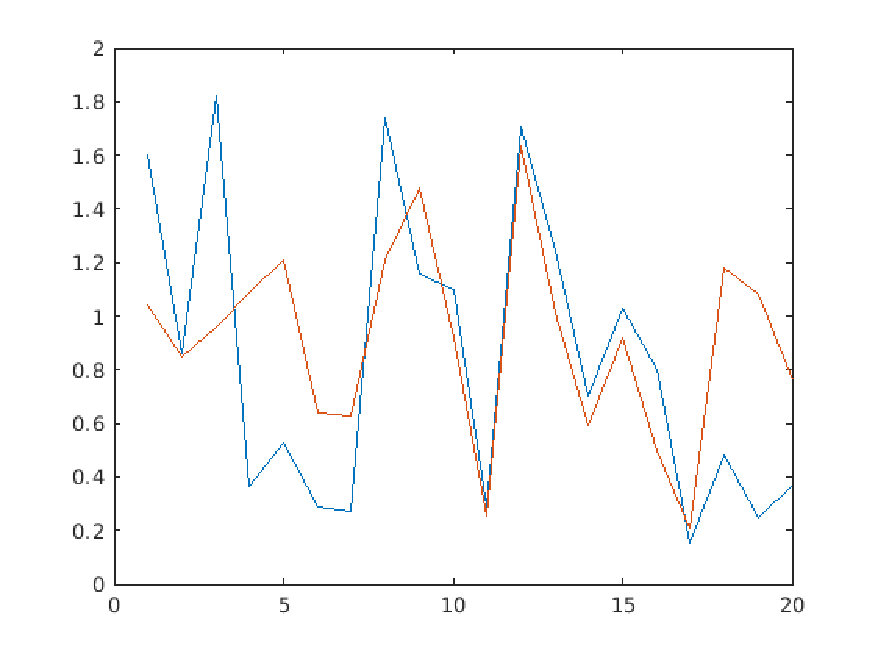
\includegraphics[width=0.5\textwidth]{simres.pdf}
 \end{center}
 \caption{Ergebnisfenster zur Daten-Visualisierung mittels plot-Befehl.}\label{abb:solman_matlab_simres}
\end{figure}

In \matlab{} existiert eine Vielzahl von Diagrammtypen und Visualisierungsm�glichkeiten, die per Kommandozeile oder graphischem Bedienerinterface (siehe Men�leiste \glqq PLOTS\grqq) angesprochen werden k�nnen.
Einige der weiterf�hrenden Plotbefehle sind unten noch einmal zusammenfassend aufgef�hrt. In den Texten und �bungen des Buches sind \mscre angegeben, die von den meisten dieser Befehle Gebrauch machen. 
\begin{table}%
\caption{Befehle f�r graphische Ausgabe.}
\smallskip
\begin{tabular}{|L{1.3cm}L{2.7cm}|L{1.3cm}L{2.7cm}|L{1.3cm}L{2.7cm}|}
\hline\noalign{\smallskip}
Funktion& Beschreibung &Funktion& Beschreibung &Funktion& Beschreibung \\
\noalign{\smallskip}\svhline\noalign{\smallskip}
\rule{0pt}{6pt} plot & 2-dimensionales Diagramm & semilogx & Diagramm mit logarithmischer x-Achse &  & schattierte Fl�che 3-dimensional\\
\hline\noalign{\smallskip}
\rule{0pt}{6pt} subplot  & Matrixanordnung von Diagrammen& semilogy & Diagramm mit logarithmischer y-Achse  & mesh & 3-dimensionales Gitterdiagramm\\
\hline\noalign{\smallskip}
\rule{0pt}{6pt} loglog  & Doppelt-logarithmisches Diagramm & surf & 3-dimensionale schattierte Oberfl�che& grid & Gitterlinien im Diagramm\\
\noalign{\smallskip}\hline\noalign{\smallskip}
\end{tabular} \label{tab:solman_matlab_plot}
\end{table}

Bitte beachten Sie die Skripte im Text f�r die verschiedenen Verwendungen dieser Befehle.

%-----------------------------------------------------------------------------------------------------------------------------------------------------------------------------
%\newpage
\section{Animationen} \label{kap:solman_matlab_film}
Mit \matlab{} kann man anschauliche Animationen erstellen. Nehmen wir als Beispiel eine sich ausbreitende ged�mpfte Welle. Man erstellt zun�chst ein Raum- und Zeitarray, gibt dann dieses Array bei jedem Zeitschritt graphisch aus und speichert den Plotframe in einem Array $M$ mit \textcolor{cyan}{\texttt{getframe}} ab. Man h�lt dann das Programm f�r eine kurze Zeit an (\zb \textcolor{cyan}{\texttt{pause}(0.1)} ). Den gesamten Ablauf kann man als Film mit 15 Bildern pro Sekunde als AVI-Datei abspeichern. Ein Beispiel ist hier angegeben:\\
\begin{lstlisting} [frame=single]
clear all
x=0:0.01:1;          % Raum-Array
t=0:0.01:1;          % Zeit-Array
nt=length(t);        % Zeitschritte
figure();
for j=1:nt 
    y=exp(-t(j)).*sin(2*pi*(x-t(j)));  % Wanderwelle
    plot(x,y,'color','r','linewidth',2); % Plot f�r jeden Zeitschritt
    ylim([-1 1]);
    grid on;
    M(j) = getframe; % speichere Movie Frames 
    pause(0.05);     % kurz pausieren
end 
movie(M, 1, 15)      % einmal mit 15 Bildern pro Sekunde abspielen
movie2avi(M,'wave'); % erstellt die Datei wave.avi 
\end{lstlisting} 
F�r die Ausgabe des Videos verwenden Sie folgenden Code:
\begin{lstlisting} [frame=single]
M = moviein(n); 
for j=l:n 
    plot 
    M(:,j) = getframe;
end 
movie(M) 
\end{lstlisting} 





%-----------------------------------------------------------------------------------------------------------------------------------------------------------------------------



\section{Skripte und benutzerdefinierte Funktionen} \label{kap:solman_matlab_files}
Ein \mscr, \zb mit \textcolor{blue}{test.m} bezeichnet, ist eine Textdatei, die \matlab-Befehle in einer geeigneten Reihenfolge enth�lt, damit sie vom Programm interpretiert und ausgef�hrt werden kann. Kommentarzeilen beginnen mit dem Prozent-Zeichen $\%$. Eine einfache m-Datei kann aus dem Befehlsfenster erstellt werden, indem der Befehl \textcolor{cyan}{$>>$ \texttt{ diary test.m }} gefolgt von mehreren Befehlen eingegeben wird, die eingeschlossen oder getestet werden sollen. Die Datei kann dann durch Eingabe von \textcolor{cyan}{$>>$ texttt{diary off }} geschlossen und �ber den \matlab-Editor oder einen anderen Texteditor aufgerufen werden. Durch Aufrufen des Namens der Datei im \matlab-Befehlsfenster; \dh durch Eingabe von \textcolor{cyan}{$>>$ \texttt{test} } wird die \matlab-Engine damit fortfahren, es zu interpretieren und die erforderliche Ausgabe zu erzeugen. Alle Fehler im Skript werden im Befehlsfenster angezeigt und k�nnen mit dem Texteditor behoben werden. 
\matlab{} hat viele eingebaute Funktionen, wie vom n�chsten Abschnitt beschrieben werden soll. Ein Benutzer kann auch eigene Funktionen erstellen. Eine Benutzerfunktion in \matlab{} ist entweder auch eine \textcolor{blue}{FunktionsName.m}-Datei oder aber sie wird am Ende des \matlab{} Files angegeben. Als Beispiel wolle wir die numerische Ableitung von $\sin\lk x\rk$ bei $x$ berechnen. Wir erstellen eine Skriptdatei mit dem Namen \textcolor{blue}{SinusAbleitung.m}: 
\begin{lstlisting} [frame=single]
function [F] = SinusAbleitung(x,del)
% Ableitung von sin(x) bei x im Intervall [x,x+del]
F = (sin(x+del)-sin(x))/del; 
\end{lstlisting} 
Sobald die Textdatei mit den obigen Zeilen unter dem Namen \textcolor{blue}{SinusAbleitung.m} gespeichert ist, kann sie �ber eine Zeile in einem \mscr aufgerufen werden. Zur Berechnung der Ableitung von $\sin\lk x\rk$ bei $x=\pi/3$ ben�tigen. Ist die Datei im Arbeitsverzeichnis gespeichert, so erh�lt man \zb:
\begin{lstlisting} [frame=single]
>>SinusAbleitung(pi/3,l.e-3) 
ans=0.5000
\end{lstlisting} 
Die Eingabe des Hilfeaufrufs im Befehlsfenster ergibt die Ausgabe:
\begin{lstlisting} [frame=single]
>>help SinusAbleitung
Ableitung von sin(x) bei x im Intervall [x,x+del]
\end{lstlisting} 
Dies ist die Zeile, die im Skript selbst als Kommentar eingef�gt wurde. Es ist wichtig, Kommentare innerhalb der Funktionen zu schreiben, um sich an ihre Verwendung zu erinnern und zu dokumentieren, dass solche Funktionen (im Arbeitsverzeichnis) vorhanden sind. 
%-----------------------------------------------------------------------------------------------
\section{Einige mathematische Funktionen}  \label{kap:solman_matlab_func}

Tabelle \ref{tab:solman_matlab_func} f�hrt einige h�ufig verwendete, vordefinierte \matlab-Funktionen auf.
\begin{table}%
\caption{Auswahl vordefinierter mathematischer Funktionen.}
\smallskip
\begin{tabular}{|L{1.3cm}L{2.7cm}|L{1.3cm}L{2.7cm}|L{1.3cm}L{3.5cm}|}
\hline\noalign{\smallskip}
Funktion& Beschreibung &Funktion& Beschreibung &Funktion& Beschreibung \\
\noalign{\smallskip}\svhline\noalign{\smallskip}
\rule{0pt}{6pt} $\tan$   & Tangens & $\min$ & kleinstes & $\tril$ &unterer dreieckiger Teil der Matrix \\
\hline\noalign{\smallskip}
\rule{0pt}{6pt} $\arcsin$   & Arcus Sinus & $\sign$ & signum & $\size$ & Gr��e einer Matrix\\
\hline\noalign{\smallskip}
\rule{0pt}{6pt} $\acos$   & Arcus Cosinus & $\length$ & L�nge eines Vektors& $\dett$ & Determinante  \\
\hline\noalign{\smallskip}
\rule{0pt}{6pt} $\arctan$   & Arcus Tangens & $\sort$ & aufsteigend sortierte Reihenfolge& $\inv$ & Inverse einer Matrix\\
\hline\noalign{\smallskip}
\rule{0pt}{6pt} $\exp$   & Exponentialfunktion & $\summ$ & Summe der Elemente einer Matrix & $\rand$ & mit Zufallszahlen gef�llte Matrix\\
\hline\noalign{\smallskip}
\rule{0pt}{6pt} $\log$   & nat�rlicher Logarithmus & $\prodd$ & Produkt der Elemente einer Matrix& $\rref$ & reduziert die Zeilenstufen einer Matrix\\
\hline\noalign{\smallskip}
\rule{0pt}{6pt} $\sin$   & Sinus & $\ceil$ & gegen positiv unendlich runden& $\diag$ & Diagonale einer Matrix extrahieren oder diagonale Matrix bilden\\
\hline\noalign{\smallskip}
\rule{0pt}{6pt} $\cos$   & Kosinus & $\max$ & gr��te Komponente & \odezd{}, \linebreak \odevf{} & L�sungsalgorithmus f�r Differentialgleichungen (Kap. \ref{kap:solman_matlab_dgl}) \\
\hline\noalign{\smallskip}
\rule{0pt}{6pt} abs   & absoluter Wert & median & Medianwert & $\eig$ & Eigenwerte und Eigenvektoren\\
\hline\noalign{\smallskip}
\rule{0pt}{6pt} $\sqrtt$   & Quadratwurzel & $\mean$ & Mittelwert & $\poly$ &Polynom\\
\hline\noalign{\smallskip}
\rule{0pt}{6pt} $\rem$   & Rest& $\std$ & Standardabweichung & $\quaddd$ & numerische Integration\\
\hline\noalign{\smallskip}
\rule{0pt}{6pt} $\round$   & auf n�chsten Integer Wert aufrunden& $\eye$ & Identit�tsmatrix & $\fzero $ & Nullstellen einer Funktion\\
\hline\noalign{\smallskip}
\rule{0pt}{6pt} $\floor$   & auf n�chsten Integer Wert abrunden& $\zeros$ & Matrix aus Nullen & $\roots$ & Wurzeln von Polynomen\\
\hline\noalign{\smallskip}
\rule{0pt}{6pt} $\modd$   & Modulo & $\ones$ & Matrix aus Einsen  & besselj & Bessel-Funktion erster Art\\
\noalign{\smallskip}\hline\noalign{\smallskip}
\end{tabular} \label{tab:solman_matlab_func}
\end{table}

Eine vollst�ndige Beschreibung der Funktionen findet man �ber die Eingabe des Hilfebefehls \mlcmd{help <Befehl>}.

%-----------------------------------------------------------------------------------------------
\newpage
\section{Programmierung} \label{kap:solman_matlab_prog}
Unter Programmierung in \matlab{} wollen wir eine Abfolge von Befehlen in einem \mscr verstehen, um wiederholte Berechnungen durchzuf�hren und Berechnungen allgemein verf�gbar zu machen. Programmieren ist \zb wichtig, wenn Schleifen und logische Anweisungen in Verbindung mit eingebauten oder benutzerdefinierten Funktionen verwendet werden. Wir geben einige Beispiele daf�r an:
\begin{lstlisting} [frame=single]
for i=l:1:1000
    x(i)=i*2;
    y(i)=sqrt(x(i));
end
\end{lstlisting} 
Die Zeilen erstellen ein 1000-Elemente-Array f�r $x$ zwischen $2$ und $2000$, f�r das die Quadratwurzel berechnet und im Array f�r $y$ gespeichert wird. In \matlab{} gibt es viel einfachere M�glichkeiten, dasselbe zu tun, das Beispiel demonstriert nur die Verwendung von Schleifen. Ein Beispiel f�r eine andere Programmierung mit dem gleichen Ergebnis:
\begin{lstlisting} [frame=single]
x = 2:2:2000;
y = sqrt(x);
\end{lstlisting} 
Ein Beispiel f�r eine if-else-Anweisung ist im Folgenden zu sehen, in dem in der Matrix $y$  alle ganzzahligen Quadratzahlen von 1 bis 1000 und in $z$ alle anderen einsortiert werden:
\begin{lstlisting} [frame=single]
ky=1;
kz=1;
for i=1:1000
    x(i)=sqrt(i);
    if abs(round(x(i))-x(i)) == 0
       y(ky) = i;
       ky = ky+1;
    else
       z(kz) = i;
       kz = kz+1;
    end
end
\end{lstlisting} 

%-----------------------------------------------------------------------------------------------
%\newpage
\section{Nullstellen von Funktionen} \label{kap:solman_matlab_roots}

Die eingebaute \matlab-Funktion \mlcmd{fzero} ist sehr n�tzlich und kann verwendet werden, um die Nullstellen einer Funktion zu bestimmen. Wir suchen \zb den Wert von $x$, bei dem die Beziehung $x = \e^{-x^2}$ erf�llt ist. 
\begin{lstlisting} [frame=single]
>>fzero('x-exp(-x^2)',0.5)
ans=0.6529
\end{lstlisting} 
wobei wir 0.5 als initialen Sch�tzwert verwendet haben. Eine vollst�ndige Beschreibung der Funktion \mlcmd{fzero} wie f�r alle anderen Funktionen finden man �ber den Hilfebefehl. Nat�rlich k�nnen wir auch die Nullstellen von benutzerdefinierte Funktionen bestimmen.\\
Ein weiteres Beispiel ist Berechnung von Wurzeln von Polynomen. Dazu kann die eingebaute Funktion \mlcmd{roots} verwendet werden. Als Beispiel berechnen wird die Nullstellen (Wurzeln) des  Polynoms 5. Ordnung $x^5+6x^3-2x+5$:
\begin{lstlisting} [frame=single]
>>x = roots([ 1 0 6 0 -2 5])
x =
  -0.0590 + 2.5180i
  -0.0590 - 2.5180i
  -1.0000 + 0.0000i
   0.5590 + 0.6897i
   0.5590 - 0.6897i
\end{lstlisting} 
Die L�sung besteht aus einer reellen und vier jeweils konjugiert komplexen Wurzeln. In Umkehrung gilt unter Verwendung des \mlcmd{poly}-Kommandos:
\begin{lstlisting} [frame=single]
>> poly(x)

ans =
    1.0000   -0.0000    6.0000   -0.0000   -2.0000    5.0000
\end{lstlisting} 

%-----------------------------------------------------------------------------------------------------------------------------------------------------------------------------
\section{Numerische Integration} \label{kap:solman_matlab_int}
Numerische Integration ist mit \matlab{} sehr einfach. Eine M�glichkeit besteht in der Nutzung der integrierten \mlcmd{quad} Funktion. Ein Beispiel daf�r ist die Integration der $\sin^2(x)$-Funktion �ber das Intervall $\lek 0, 2\pi\rek$ :
\begin{lstlisting} [frame=single]
>>quad('sin(x).^2',0, 2*pi);
ans =3.1416
\end{lstlisting} 
Hier haben wir eine vom Benutzer eingebauten Funktion inline benutzt. Man beachte die Operatoren f�r die elementweise Ausf�hrung (\zb .*). Alternativ kann man die zu integrierende Funktion �ber eine \textit{inline} Anweisung oder ein Handle @ auf eine zuvor definierte Funktion erzeugen.
\begin{lstlisting} [frame=single]
>> g=inline('2*x.^3+x.^5.*sin(x).^2');
>> quad(g,0,pi)
ans=86.4451 
\end{lstlisting} 
Hier wurde die Funktion $2 x^3+x^5 \sin^2(x) $ auf $\lek 0, \pi\rek$ integriert. Mit Handle sieht das entsprechende \mscr folgenderma�en aus:
\begin{lstlisting} [frame=single]
int3 = quad(@myfunc,0,pi);
function gh = myfunc(x)
    gh = 2*x.^3+x.^5.*sin(x).^2;
end
int3=86.4451 
\end{lstlisting} 


%-----------------------------------------------------------------------------------------------------------------------------------------------------------------------------
%\newpage
\section{Differentialgleichungen} \label{kap:solman_matlab_dgl}

Eine wesentliche F�higkeit von \matlab{} ist die numerische L�sung von Differentialgleichungen\index{Differentialgleichung} (DGL). Bei der numerischen L�sung von DGL bestimmt man ausgehend von Anfangsbedingungen\index{Anfangsbedingungen} (AB) eine Folge von Wertepaaren $(t_0, y_0)$, $(t_1, y_1)$, $(t_2, y_2), \ldots $, die den Verlauf der gesuchten Funktion $y(t)$ ann�hern sollen. In \matlab{} wird unterschieden zwischen gew�hnlichen Differentialgleichungen\index{Differentialgleichung!gew�hnliche} (ODE, \textit{Ordinary Differential Equations}), differential-algebraischen
Gleichungen \index{Differential-Algebraisches System} (DAE, \textit{Differential Algebraic Equations}) \ua Die in \matlab{} enthaltenen numerischen L�sungsalgorithmen (\textit{Solvers})\index{Solver} k�nnen f�r eine
Vielzahl von Systemen eingesetzt werden, die durch Differentialgleichungen beschreibbar sind. Ausf�hrliche Behandlung zu Differentialgleichungen und deren numerischer L�sung finden sich in \cite{Riley2006, Felder2016, Fischer2014}.

\subsection{Gew�hnliche Differentialgleichungen (ODE)} \label{kap:solman_matlab_ODE}
 
Mathematisch l�sst sich eine gew�hnliche Differentialgleichung mit dem Zustandsvektor $\vec{Y}$
und dem Zeitargument $t$, einer beliebigen vektorwertigen Funktion $\vec{f}$ und dem Anfangsbedingungen $\vec{Y}_0$
zum Zeitpunkt $t_0$ als Differentialgleichungssystem erster Ordnung darstellen:
	\begin{align}
\frac{\D \vec{Y}}{\D t} = \vec{f}(t,\vec{Y}) ~~~~\text{mit} ~~~~\vec{Y}(t_0) = \vec{Y}_0\,. \label{eq:solman_matlabdgl01}
	\end{align}
\matlab{} hat die F�higkeit, solche Differentialgleichungen mit eingebauten Funktionen wie \textcolor{cyan}{\texttt{ode45}} oder \textcolor{cyan}{\texttt{ode23}} \ua zu l�sen. Wir wollen als Beispiel ein eindimensionales Problem l�sen. Als Beispiel haben wir die DGL $\dot{y}=(y-t^2)\e^{-t}$ f�r $y\lk t\rk$ auf dem Intervall $\lek 0,20\rek$ mit der Anfangsbedingung $t=0, y=1$ ausgew�hlt. In \matlab{} kann dies wie folgt erreicht werden: 
\begin{lstlisting} [frame=single]
tspan=linspace(0,10);
[t,y]=ode45(@myfunc,tspan,1 ); 
figure()
plot(t,y)
function f = myfunc(t,y)
  f=(y-t.^2).*exp((-t));
end
\end{lstlisting} 
Zur L�sung von Differentialgleichungen gem�� \eqref{eq:solman_matlabdgl01} stehen in \matlab{} verschiedene Algorithmen (Solver) zur Verf�gung. Die \matlab-Solver unterscheiden sich hinsichtlich ihres Verhaltens bei sogenannten steifen Differentialgleichungen.\index{Differentialgleichung!steife} Eine Differentialgleichung wird als steif (\textit{stiff}) bezeichnet, wenn die Verfahren wegen ihres beschr�nkten Stabilit�tsgebietes erhebliche Genauigkeitsprobleme haben oder wenn Schaltvorg�nge zu ber�cksichtigen sind. Diese treten bis auf wenige Ausnahmen in den im Buch betrachteten F�llen nicht auf. Bei der Wahl der Integrationsverfahren hat sich deshalb folgendes Vorgehen bew�hrt. Zuerst
w�hlt man den Solver \textcolor{cyan}{\texttt{ode45}}, welcher eine Implementierung eines expliziten Runge-Kutta-Verfahrens\index{Runge-Kutta-Verfahren} 5. Ordnung ist (siehe die \onlineZ \bzw \cite{Riley2006, Fischer2014, Natt2020}). Dann �berpr�ft man die Ergebnisse auf Stabilit�t und kann gegebenenfalls einen Solver wie \textcolor{cyan}{\texttt{ode15s}} oder \textcolor{cyan}{\texttt{ode23s}} zur Berechnung probieren. Wir empfehlen, sich die Skripte des Buches f�r die einzelnen Beispiele anzuschauen oder die Befehle \textcolor{cyan}{\texttt{ help ode45}} \bzw \textcolor{cyan}{\texttt{ode15s}} in das Befehlsfenster einzugeben, um weitere Informationen und Details zu erhalten. 

Bisher haben wir nur DGL \bzw DGL-Systeme mit ersten Ableitungen betrachtet. In der Physik und insbesondere in der Mechanik treten aber vorwiegend DGL-Systeme zweiter Ordnung nach der Zeit auf, \dh wir haben eigentlich System der Form:
	\begin{align}
\frac{\D^2 \vec{\tilde{Y}}}{\D t^2} = \vec{f}(t,\vec{\tilde{Y}}) ~~~~\text{mit} \vec{}(t_0) = \vec{\tilde{Y}}_0\,. \label{eq:solman_matlabdgl02}
	\end{align}
Diese kann man aber problemlos in ein System 1. Ordnung gem�� \eqref{eq:solman_matlabdgl01} �berf�hren. Wir wollen das f�r ein DGL-System f�r 3 Koordinaten $(\tilde{Y}_1, \tilde{Y}_2, \tilde{Y}_3)$ zeugen.
Wir schreiben dazu:
\begin{align}
	Y_1 &= \tilde{Y}_1,~~~~ &Y_2 = \D \tilde{Y}_1 / \D t \nonumber \\
	Y_3 &= \tilde{Y}_2,~~~~ &Y_4 = \D \tilde{Y}_4 / \D t  \label{eq:solman_matlabdgl03} \\
	Y_5 &= \tilde{Y}_3,~~~~ &Y_6 = \D \tilde{Y}_6 / \D t \nonumber \,.
\end{align}
Das �quivalente $2n$-dimensionale DGL-System 1. Ordnung zum $n$-dimensionalen System 2.Ordnung \eqref{eq:solman_matlabdgl02} lautet dann.
\begin{align}
	\dot{Y}_1 &= Y_4 = f_1(Y_4)~ , ~~&\dot{Y}_4 = f_4(t, \vec{Y}) \nonumber \\
	\dot{Y}_2 &= Y_5 = f_2(Y_5)~ , ~~&\dot{Y}_5 = f_5(t, \vec{Y})  \label{eq:solman_matlabdgl04} \\ 
	\dot{Y}_3 &= Y_6 = f_3(Y_6)~ , ~~&\dot{Y}_6 = f_6(t, \vec{Y}) \nonumber \,.
\end{align}
Dieses Verfahren haben wir \zb bei der Berechnung der Wirkungen der Corioliskraft im Kapitel Physik der Bewegung angewendet. Dort wurde die die Funktion $\vec{f}$ mit Parametern versehen und als \textcolor{cyan}{\texttt{CoriolisDGLS(t,Y,Omeg,Cphi,Sphi,G,Eta)}} definiert:
\begin{lstlisting} [frame=single]
% Differentialgleichungssystem f�r Corioliskraft
function dY = CoriolisDGLS(t,Y,Omeg,Cphi,Sphi,G,Eta)
  dY    = zeros(6,1);
  dY(1) = Y(4); dY(2) = Y(5); dY(3) = Y(6);
  vbet  = sqrt(Y(4)^2+Y(5)^2+Y(6)^2);
  dY(4) = 2*Omeg*Sphi*Y(5)-Eta*vbet*Y(4);
  dY(5) = -2*Omeg*Sphi*Y(4)-2*Omeg*Cphi*Y(6)-Eta*vbet*Y(5);
  dY(6) = 2*Omeg*Cphi*Y(5)-G-Eta*vbet*Y(6);  
end
\end{lstlisting} 
Wir hatten bisher auch implizit angenommen, dass das DGL-System in expliziter Form, \dh in der Form $\D \vec{Y}/\D t = \vec{f}(t,\vec{Y})$ vorliegt. H�ufig aber findet man es eher in der Form:
\begin{equation} 
    \mathbb{M}(t,\vec{Y}) \dot{\vec{Y}} = f(t,\vec{Y})\,, \label{eq:solman_matlabdgl05}
\end{equation} 
worin $\mathbb{M}$ die sogenannte Massen-Matrix ist. %Wir finden eine solche Form \ua in der \probref {bew_Hantelwurf}:
\begin{align*}
    \begin{bmatrix}
          1 & 0  & 0 & 0 & 0 & 0 \\
          0 & m_1+m_2  & 0 & 0 & 0 & -m_2\,L\sin Y_5 \\
          0 & 0  & 1 & 0 & 0 & 0 \\
          0 & 0  & 0 & m_1+m_2 & 0 & m_2\,L\cos Y_5\\
          0 & 0  & 0 & 0 & 1 & 0 \\
          0 & -L\sin Y_5  & 0 & L \cos Y_5 & 0 & L^2 \\
    \end{bmatrix}
    \begin{bmatrix}
          \dot{Y}_1 \\
          \dot{Y}_2 \\
          \dot{Y}_3 \\
          \dot{Y}_4 \\
          \dot{Y}_5 \\
          \dot{Y}_6 \\
    \end{bmatrix}
    =
    \begin{bmatrix}
          Y_2 \\
          m_2\,L\,{Y_6}^2 \cos Y_5 \\
          Y_4 \\
          m_2\,L\,{Y_6}^2 \sin Y_5 - (m_1+m_2)\,g\\
          Y_6 \\
          -g\,L\cos Y_5\\
    \end{bmatrix}
\end{align*} 
Das System kann also in der Form einer Matrixgleichung gem�� \eqref{eq:solman_matlabdgl05} geschrieben werden. Die weitere Berechnung der L�sung diese DGL-Systems mittels \matlab{} mit dem \texttt{ode45} Solver ist v�llig analog mit der beschriebenen Vorgehensweise zur L�sung von Gleichungssystemen der Form \eqref{eq:solman_matlabdgl04}. Lediglich muss hier beim Setzen der Optionen f�r den \texttt{ode45} Solver mittels \textcolor{cyan}{\texttt{odeset}} die Massenfunktion \textcolor{cyan}{\texttt{'Mass'}}  ($M = \text{Mass}(t,Y,P)$) aufgerufen werden. Dabei wird mit $P$ auch eine Struktur mit dem Parametersatz �bergeben.%in unserem Fall $(m_1, m_2, L, g)$.
\begin{lstlisting} [frame=single]
opts = odeset('Mass',@(t,Y) Mass(t,Y,P1));
[t,Y1] = ode45(@(t,Y) f(t,Y,P1),tspan,Y01,opts);
function M = Mass(t,q,P)
% Extrahiere Parameter
m1 = P.m1; m2 = P.m2; L = P.L; g = P.g;
% Massen-Matrix
M = zeros(6,6);
M(1,1) = 1;
M(2,2) = m1 + m2;
M(2,6) = -m2*L*sin(q(5));
M(3,3) = 1;
M(4,4) = m1 + m2;
M(4,6) = m2*L*cos(q(5));
M(5,5) = 1;
M(6,2) = -L*sin(q(5));
M(6,4) = L*cos(q(5));
M(6,6) = L^2;
end
% DGL Funktion f
function dYdt = f(t,Y,P) 
% Extrahiere Parameter
m1 = P.m1; m2 = P.m2; L = P.L; g = P.g;
% DGL
dYdt = [Y(2)
        m2*L*Y(6)^2*cos(Y(5))
        Y(4)
        m2*L*Y(6)^2*sin(Y(5))-(m1+m2)*g
        Y(6)
        -g*L*cos(Y(5))];
end
\end{lstlisting} 

\textbf{\textit{Setzen der Optionen f�r Solver:}} \\
Unter Ber�cksichtigung von Optionseinstellungen f�r den Solver und Parameter�bergaben an die Funktionen \textcolor{cyan}{\texttt{dYdt}} lauten die allgemeinen Aufrufe der
verschiedenen Solver:
\begin{lstlisting} [frame=single]
options = odeset(�name1�,wert1,�name2�,wert2,...);
[t,Y] = solver(@dYdt,tspan,Y0,options,p1,p2,...);
\end{lstlisting} 
Die Parameter p1, p2, ... werden an die Funktion dYdt und an alle evtl. in den Optionen
definierten Funktionen als zus�tzliche Argumente �bergeben. Eine Struktur \textcolor{cyan}{\texttt{options}} mit Standardvorbelegungen
wird durch das Kommando \textcolor{cyan}{\texttt{odeset}} erzeugt, damit wird das Verhalten der Solver gesteuert. Folgende Werte k�nnen gesetzt werden.

\begin{table}%
\caption{Auswahl von Werten (Standardwerten) f�r das Setzen von Optionen mit \textcolor{cyan}{\texttt{odeset}}.}
\smallskip
\begin{tabular}{|L{4cm}|L{6cm}|}
\hline\noalign{\smallskip}
Optionsparameter  & Wert  \\
\noalign{\smallskip}\svhline\noalign{\smallskip}
\rule{0pt}{6pt} AbsTol &[ positive scalar or vector \textcolor{red}{(1e-6)} ] \\
\hline\noalign{\smallskip}
\rule{0pt}{6pt} RelTol &[ positive scalar \textcolor{red}{(1e-3)} ]\\
\hline\noalign{\smallskip}
\rule{0pt}{6pt} Mass &[ matrix | function\_handle ]\\
\hline\noalign{\smallskip}
\rule{0pt}{6pt} Events &[ function\_handle ] \\
\hline\noalign{\smallskip}
\rule{0pt}{6pt} MassSingular &[ yes | no | \textcolor{red}{(maybe)} ]\\
\hline\noalign{\smallskip}
\rule{0pt}{6pt} Events &[ function\_handle ] \\
\hline\noalign{\smallskip}
\rule{0pt}{6pt} Jacobian &[ matrix | function\_handle]\\
\hline\noalign{\smallskip}
\rule{0pt}{6pt} NormControl &[ on | \textcolor{red}{(off)} ]\\
\hline\noalign{\smallskip}
\rule{0pt}{6pt} Events &[ function\_handle ] \\
\hline\noalign{\smallskip}
\rule{0pt}{6pt} NonNegative &[ vector of integers ]\\
\hline\noalign{\smallskip}
\rule{0pt}{6pt} Events &[ function\_handle ] \\
\hline\noalign{\smallskip}
\rule{0pt}{6pt} InitialStep &[ positive scalar ]\\
\hline\noalign{\smallskip}
\rule{0pt}{6pt} MaxStep &[ positive scalar ]\\
\hline\noalign{\smallskip}
\rule{0pt}{6pt} OutputFcn &[ function\_handle ]\\
\hline\noalign{\smallskip}
\rule{0pt}{6pt} OutputSel &[ vector of integers ] \\
\hline\noalign{\smallskip}
\rule{0pt}{6pt} InitialSlope &[ vector ] \\
\noalign{\smallskip}\hline\noalign{\smallskip}
\end{tabular} \label{tab:solman_matlab_odeset}
\end{table}
In eckigen Klammern werden die m�glichen Werte \bzw rot in runden Klammern die
Standardwerte angezeigt. Die genauere Bedeutung der einzelnen Parameter der Options-Struktur wird in den einzelnen \mscren erl�utert und auch ersichtlich. Im Allgemeinen braucht man nur wenige Optionen zu ver�ndern und kann vielfach mit Standardwerten arbeiten. F�r weitere Details verweisen wir auf das Hilfemen� von \matlab{}. \\

\textbf{\textit{Event}-Behandlung:} \\
In vielen technischen Systemen spielen Schaltvorg�nge oder Unstetigkeiten
eine wichtige Rolle. Typische Beispiele sind Haftreibungsvorg�nge, Sto�vorg�nge oder 
das Verschwinden von Zwangskr�ften (siehe Kap. Physik der Bewegung).
Die numerischen Integrationsverfahren d�rfen �ber solche
Unstetigkeitsstellen nicht einfach hinwegintegrieren. Die Solver in \matlab{}
sind zu diesem Zweck mit Mechanismen zur Detektion solcher Unstetigkeiten, so
genannter \textit{Events}, ausgestattet. Die Solver sind in der Lage, w�hrend der Integration
die Schrittweite so anzupassen, dass die Nullstellen einer Event-Funktion exakt mit einem Integrationsschritt
getroffen werden. Wenn die Nullstelle erreicht wird, kann die Integration
entweder ganz normal fortgesetzt oder angehalten werden. Die Option \textcolor{cyan}{\texttt{events}} wird
benutzt, um die Funktion anzugeben, deren Nullstellen detektiert werden sollen. Die
Funktion muss die folgende Form besitzen:
\begin{lstlisting} [frame=single]
function [value,isterminal,direction] = ereignis(t,Y,p1,p2,...)
\end{lstlisting} 
Die Funktion \textit{Event} wird mit dem aktuellen Zeitpunkt t, dem Zustandsvektor Y und
evtl. weiteren Parametern p1, p2, ... aufgerufen. Die R�ckgabewerte haben die folgende
Bedeutung:
\begin{itemize}
	\item \textcolor{cyan}{\texttt{value}} ist ein Vektor, dessen Nulldurchg�nge vom Solver �berwacht werden. Das Element \textcolor{cyan}{\texttt{value(i)}} wird als i-tes Ereignis bezeichnet.
	\item \textcolor{cyan}{\texttt{isterminal(i)=1}} bedeutet, dass bei einem Nulldurchgang von \textcolor{cyan}{\texttt{value(i)}}= die numerische
Integration zu beenden ist. Wenn \textcolor{cyan}{\texttt{isterminal(i)=0}} ist, wird die Integration fortgesetzt.
	\item \textcolor{cyan}{\texttt{direction(i)=0}} hei�t, dass alle Nulldurchg�nge von \textcolor{cyan}{\texttt{value(i)}} zu detektieren
sind; bei \textcolor{cyan}{\texttt{direction(i)=1}} werden nur Nulldurchg�nge negativ zu positiv bzw.
bei \textcolor{cyan}{\texttt{direction(i)=-1}} nur Nulldurchg�nge von positiv zu negativ detektiert.
\end{itemize}
Die �berwachung von Ereignissen wird durch die Option \textcolor{cyan}{\texttt{events}} aktiviert:
\begin{lstlisting} [frame=single]
options = odeset(�Events�, @ereignis);
\end{lstlisting} 
Durch die Verwendung der Option \textcolor{cyan}{\texttt{events}} gibt der Solver weitere R�ckgabewerte aus:
\begin{lstlisting} [frame=single]
[t,Y,TE,YE,IE] = solver(@dYdt,tspan,Y0,options,p1,p2,...);
\end{lstlisting} 
Im Spaltenvektor TE werden die Zeitpunkte des Auftretens eines Events aus der Funktion
\textcolor{cyan}{\texttt{Ereignis}} zur�ckgegeben. Die Zeilen von YE enthalten den L�sungsvektor zu diesen
Event-Zeitpunkten. Die Werte in IE geben den Index des Elements \textcolor{cyan}{\texttt{value(IE)}} der
Ereignisfunktion an, bei der ein Nulldurchgang stattfand.\\

\textbf{Feste Ausgabeschrittweite der Solver:} \\
Der Solver \textcolor{cyan}{\texttt{ode45}} arbeitet mit einem verbesserten Runge-Kutta-Verfahren, mit dem die Schrittweite gesteuert werden.
Wegen dieser automatischen Schrittweitensteuerung legt textcolor{cyan}{\texttt{ODE45}} selbst fest, in wie viele Zeitschritte das vorgegebene Zeitintervall unterteilt wird. 
Die Zeitschritte sind im Allgemeinen nicht mehr �quidistant, deshalb ist die Matrix der Ergebnisse Y immer im Zusammenhang mit dem Ergebnisvektor
t zu sehen. Die L�nge des Ergebnisvektors kann gegebenenfalls mit der \matlab-Funktion \textcolor{cyan}{\texttt{length}} erfragt werden. H�ufig braucht man aber doch �quidistante Ausgabewerte. Hier gibt es zwei M�glichkeiten.\\
\begin{itemize}
	\item \textcolor{cyan}{\texttt{odeset}} ohne Eventfunktion:\\
                In diesem Fall kann man durch explizite Angabe der Range in �quidistanter Form eine �quidistante Ausgabe f�r Y erzwingen.
\begin{lstlisting} [frame=single]
Y0 = [100,0]
tspan = linspace(1,5,101)
opt=odeset('AbsTol',1.e-9,'RelTol',1.e-7);           
[t,Y]=ode45(@DGL,tspan,Y0,opt); 
plot(t,Y(:,1)); %t, hat �quidistante Elemente
function dY = DGL(t,Y)
g  = 9.81;  
dY = [Y(2); -g];
end
\end{lstlisting} 

	 \item \textcolor{cyan}{\texttt{odeset}} mit Eventfunktion:\\
                Das gerade beschriebene Verfahren funktioniert in diesem Fall wegen der Event bezogenen Schrittsteuerung nicht.
                Hier hilft nur, m�glichst viele Ausgabewerte zu berechnen und dann zu interpolieren.
                Wir haben dies \zb in \mlbewref{MurphysLaw.m} ausgef�hrt und geben hier das Listing an:
\begin{lstlisting} [frame=single]
options1=odeset('AbsTol',1.e-9,'RelTol',1.e-7,'events',@MyEvent1);
[t,Y,TE,YE,IE]=ode45(@dgl_Brett1,tspan,AB,options1,P1); 
% t,Y sind nicht �quidistant
% interpolieren, um �quidistante intervalle f�r den ode output zu erhalten
Yeq=interp1(t,Y,tspan); % Yeq ist nun �quidistanter
\end{lstlisting} 

\end{itemize}

\subsection{Differential-Algebraische Gleichungen (DAE)} \label{kap:solman_matlab_DAE}

H�ufig lassen sich DGLen der Mechanik durch eine Differentialgleichung
mit Masse-Matrix gem�� Gleichung \eqref{eq:solman_matlabdgl05} darstellen.
In der zeit- und zustandsabh�ngigen Masse-Matrix $\mathbb{M}$sind typischerweise Massen und
Tr�gheitsmomente des Systems enthalten. Wenn die Masse-Matrix nicht
singul�r\index{Matrix!nicht-singul�re} ist (siehe die \onlineZ), kann die Gleichung umgeformt werden und es existiert
eine L�sung f�r alle Anfangsbedingungen $t_0$ und $\vec{Y}_0$.
Bei nicht singul�rer Masse-Matrix sind alle Solver in der Lage, ein System gem�� Gleichung
\eqref{eq:solman_matlabdgl05} zu l�sen. 

Bei singul�rer Matrix\index{Matrix!singul�re} $\mathbb{M}(t,\vec{Y})$ stellt Gleichung \eqref{eq:solman_matlabdgl05}
eine differential-algebraische Gleichung (DAE)\index{Differential-Algebraisches System}  dar, die nur dann eine L�sung besitzt, wenn der Anfangswert
$\vec{Y}_0$ konsistent mit der DAE ist. Das bedeutet, es muss eine Anfangssteilheit
$\D \vec{Y}_0 / \D t$ existieren, so dass 
	\[\mathbb{M}(t,\vec{Y}_0) \D \vec{Y} / \D t |t_0 = f(t_0, )
	\]
ist. Bei nicht konsistenter Anfangsbedingung versucht der Solver in deren N�he eine konsistente zu finden
und das Problem mit diesen neuen Anfangswerten zu l�sen. DAEs k�nnen nur mit
den Solvern \textcolor{cyan}{\texttt{ode15s}} und \textcolor{cyan}{\texttt{ode23t}} behandelt werden. Der Solver \textcolor{cyan}{\texttt{ode23s}} kann nur
DAEs mit konstanter Masse-Matrix l�sen. In der Option \textcolor{cyan}{\texttt{Mass}} muss entweder eine
konstante Matrix oder ein Zeiger auf eine Funktion zur Ermittlung der Masse-Matrix
enthalten sein.\\
Ein nicht-getriebenes Pendel der L�nge L mit Reibung $F_\text{R}$ soll als Beispiel f�r eine Differentialgleichung
mit Masse-Matrix dienen und wird in die Form \eqref{eq:solman_matlabdgl05} gebracht. Zus�tzlich wird
angenommen, dass die Masse $m$ des Pendels mit der Zeit exponentiell abnimmt und
das Pendel nicht angetrieben wird. 
Als Differentialgleichungssystem mit Masse-Matrix ergibt sich:
\begin{align}
\dot{Y}_1 &= Y_2 ~~,~~m(t) \dot{Y}_1 = -m(t)\frac{g}{L}\sin{Y_1} - \frac{2\,F_\text{R}}{\pi L}\sin{Y_1} \arctan{10 Y_2} \, \label{eq:solman_matlabdgl07} \\
\rightarrow \mathbb{M}(t,\vec{Y}) &=  \begin{pmatrix}
        1 & 0 \\
        0 & m(t) 
        \end{pmatrix} \,.\label{eq:solman_matlabdgl08}
\end{align}
Die Funktion \textcolor{cyan}{\texttt{Ydot\_pendelmass}} repr�sentiert die rechten Seiten der Gleichungen in \eqref{eq:solman_matlabdgl07}.
\begin{lstlisting} [frame=single]
% DAE Pendel
% Daten, Anfangswerte, Zeitspanne, Optionen
L = 5; m0 = 30; g = 9.81; FR = 4; T = 15;
Y0 = [15/360*2*pi; 0];
tspan = [0 20]; 
%Damit der Solver die Masse-Matrix verwenden kann, muss sie ueber die Option Mass auf
%@mass gesetzt werden. Die Loesung erfolgt mit Solver ode15s 
options = odeset('Mass', @mass);
[t Y] = ode15s(@Ydot_pendelmass,tspan,Y0,options,L,m0,g,FR,T);
%-----------------------------------------------
% Ydot_pendelmass, DGL
function Ydot = Ydot_pendelmass(t,Y,L,m0,g,FR,T)
  m = m0*exp(-t/T);
  Ydot = [Y(2); -m*g/L*sin(Y(1)) - FR*2/pi*atan(10*Y(2))/L];
end
%-----------------------------------------------
% mass.m
% Berechnung der Masse-Matrix wird in der Funktion mass
% realisiert. Daten des Pendels als Parameter vom Solver uebergeben.
function M = mass(t,Y,L,m0,g,FR,T)
  M = [1 0; 0 m0*exp(-t/T)];
end
\end{lstlisting} 

\begin{lstlisting} [frame=single]
% Ausgabe
figure()
plot (t,Y(:,1));
hold on
plot (t,Y(:,2));
figure()
plot (t,m0*exp(-t/T));
\end{lstlisting} 
Als L�sung f�r $\varphi(t)=$Y(:,1) und $\dot{\varphi}(t)=$Y(:,2) �ber die Zeitspanne von 20 s ergibt sich der in \figref{solman_matlab_DAE}a dargestellte Verlauf.
In \figref{solman_matlab_DAE}b ist der zugeh�rige Masseverlauf dargestellt.
Eine etwas komplexere DAE haben wir im Kapitel Physik der Bewegung von K�rpern (Band I) mit dem \mscr \mlbewref{TrebSimDAE.m} behandelt:
\begin{lstlisting} [frame=single]
% Runge-Kutta-Verfahren-MATLAB ODE15s
opts = odeset('Mass',@(t,Y) Mass1(t,Y,P),'RelTol',1e-6);
[t,Y] = ode15s(@(t,Y) F1(t,Y,P),tv,AB1,opts);
% -------------------------------------------------------
% Massen-Matrix f�r Schleifphase (mit Zwangsbedingung)
function M = Mass1(t,q,P)
% Parameter extrahieren
JG  = P.JG; JW  = P.JW; JbW = P.JbW; JBG = P.JBG;
J0  = P.J0; b   = P.b; lW  = P.lW;
% Massen-Matrix aufstellen
M = zeros(7,7);
M(1,1) = 1; M(2,2) = J0; M(3,3) = 1; 
M(4,4) = JG; M(5,5) = 1; M(6,6) = JW; 
M(2,4) = +JBG*cos(q(1)-q(3)); M(4,2) = M(2,4);
M(2,6) = -JbW*cos(q(1)-q(5)); M(6,2) = M(2,6);
M(7,2) = -b*cos(q(1)); M(7,6) = lW*cos(q(5));
M(2,7) = M(7,2); M(6,7) = M(7,6);
end
% -------------------------------------------------------
% DGL Funktion
function dYdt = F1(t,Y,P)
% Parameter extrahieren
LG  = P.LG;  lW  = P.lW;  MG  = P.MG; mW  = P.mW; 
JBG = P.JBG; JbW = P.JbW; g   = P.g;   U0  = P.U0; b   = P.b; 
% DGL
dYdt = [Y(2);
 -JBG*Y(4)^2*sin(Y(1)-Y(3))+JbW*Y(6)^2*sin(Y(1)-Y(5))-U0*cos(Y(1));
 Y(4); 
 +JBG*Y(2)^2*sin(Y(1)-Y(3)) - MG*LG*g*cos(Y(3));
 Y(6);
 -JbW*Y(2)^2*sin(Y(1)-Y(5)) - mW*lW*g*cos(Y(5));
 -b*Y(2)^2*sin(Y(1)) + lW*Y(6)^2*sin(Y(5))];
end
\end{lstlisting} 

\begin{figure}[!htpb]
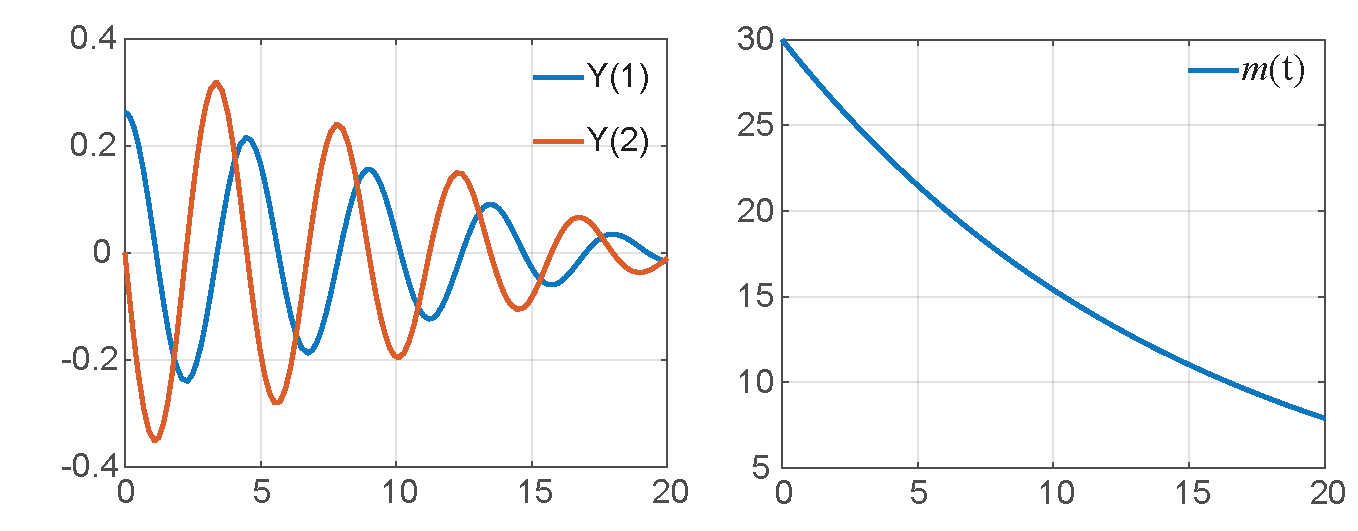
\includegraphics[width=\textwidth]{ExampleDAE.pdf}
\caption[Ergebnisfenster des \matlab-Programms f�r DAE-Berechnung.]{Ergebnisfenster des \matlab-Programms f�r DAE-Berechnung \eqref{eq:solman_matlabdgl07}.}\label{abb:solman_matlab_DAE}
\end{figure}

\subsection{Differentialgleichung mit Delay-Zeiten (DDE)} \label{kap:solman_matlab_DDE}

\newpage
\subsection{Partielle Differentialgleichungen (PDE)} \label{kap:solman_matlab_PDG}

In Anlehnung an die \matlab-Onlinehilfe unter
\url{https://de.mathworks.com/help/matlab/math/partial-differential-equations.html}
sei hier ein einfaches Beispiel der W�rmeleitungsgleichung 
\begin{align}
  \frac{\partial u}{\partial t} = 0.1\cdot\frac{\partial^2 u}{\partial x^2}
\end{align}
angegeben. Es handelt sich um eine parabolische Differentialgleichung, die die �rtliche und zeitliche �nderung der Temperatur $u(x,t)$ wiedergibt.
Dies mag ein eindimensional modellierter Stab sein, dessen Temperatur auf halben Niveau startet und dessen Enden hoher \bzw niedriger Temperatur ausgesetzt werden.
F�r die \matlab-Simulation sind die Angabe von (�rtlichen) Randbedingungen $u(0,t) = 0$ und $u(1,t) = 1$
\begin{lstlisting} [frame=single]
function [pl,ql,pr,qr] = WlgRandbedingungen(xl,ul,xr,ur,t)
  pl = ul;
  ql = 0;
  pr = ur - 1;
  qr = 0;
end
\end{lstlisting} 
sowie der (zeitlichen) Anfangsbedingung $u(x,0)=0.5$
\begin{lstlisting} [frame=single]
function u0 = WlgAnfangswerte(x)
  u0 = 0.5;
end
\end{lstlisting} 
erforderlich. Ebenso wie die Definition der PDE (mit diversen Anpassungsfaktoren $c,s$ f�r allgemeinere Problemklassen)
\begin{lstlisting} [frame=single]
function [c,f,s] = WlgPDE(x,t,u,dudx)
  c = 1;
  f = 0.1*dudx;
  s = 0;
end
\end{lstlisting} 
erfolgt dies in jeweils eigenen Funktions-Skripten. Der Aufruf des eigentlichen PDE-Solvers \mlcmd{pdepe} erfolgt mit
\begin{lstlisting} [frame=single]
% PDG Solver
x = linspace(0,1,200);
t = linspace(0,1,200);
u = pdepe(0,@WlgPDE,@WlgAnfangswerte,@WlgRandbedingungen,x,t)';
colormap hot
imagesc(t,x,u)
colorbar
xlabel('t')
ylabel('x')
\end{lstlisting} 
und liefert den �rtlichen und zeitlichen Temperaturverlauf f�r $0\le x\le 1$ und $0\le t \le 1$, siehe Abb. \ref{abb:solman_matlab_PDE}.
\begin{figure}[!htpb]
 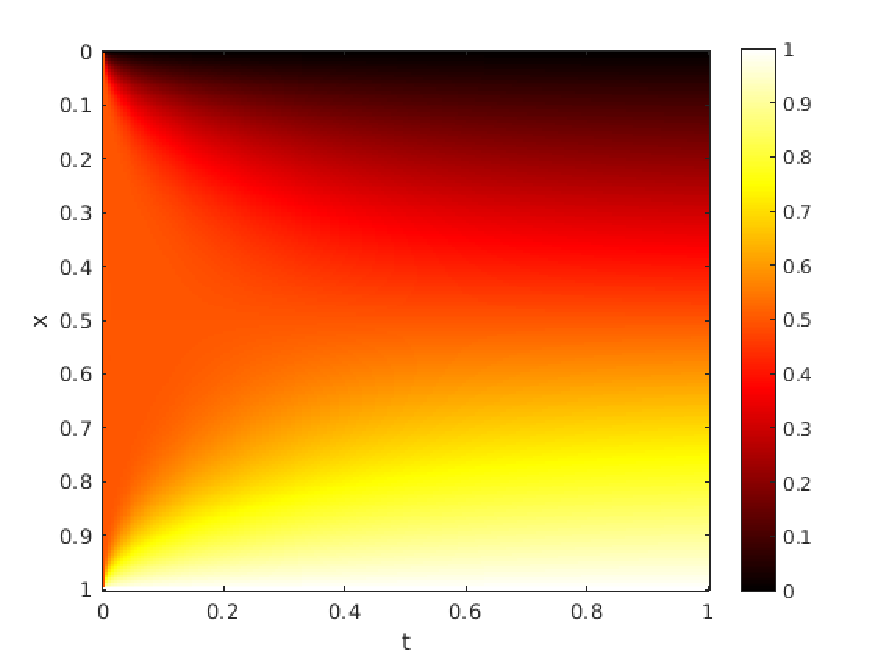
\includegraphics[width=\textwidth]{WlgPDGL.pdf}
 \caption[Ergebnisfenster des \matlab-Programms f�r PDE-Berechnung.]{Ergebnisfenster des \matlab-Programms f�r PDE-Berechnung.}
\end{figure}

%%%%%%%

\newpage
\section{Symbolische Berechnung}\label{kap:solman_matlab_symb}
\matlab{} kann symbolische Rechnungen durchf�hren. Geben Sie \texttt{help symbolic}  in die Befehlszeile ein,
Eine Liste der verf�gbaren Funktionen wird angezeigt, wenn die Symbolic Math Toolbox mit der Version von \matlab{} verf�gbar ist. Ein einfaches Beispiel f�r eine symbolische Operation ist das Plotten der Funktion $y = 2 t \sin(t/2/\pi)$. Dies wird durch Eingabe der folgenden Zeilen erreicht: \\
\begin{lstlisting} [frame=single]
>> syms t a
>> a = 2
>> y=2*t
y=2*sqrt(t/a)*sin(t/2)
ezplot(t,y)
\end{lstlisting} 
Ein weiteres Beispiel ist das Plotten der Funktion $y = 2 t^2 \e^{ -a t^2}$ und ihrer Ableitung. Dies wird in einem \mscr wie folgt realisiert:\\
\begin{lstlisting} [frame=single]
syms t y f a
y=2*t^2*exp(-a*t^2)
f=diff(y,t)
f = 4*t*exp(-a*t^2) - 4*a*t^3*exp(-a*t^2)  % Ergebnis
a=0.5000;
ezplot(t,eval(y),[-5 5])
hold on
ezplot(t,eval(f),[-5 5])
\end{lstlisting} 
Das Ergebnis ist in \figref{solman_matlab_symb} zu sehen. Weitere Beispiele f�r symbolische Berechnungen sind in den \matlab-Lehrb�chern \cite{Schweizer2016, Attaway2013} oder im Hilfemen� von \matlab{} verf�gbar.
\begin{figure}[!htpb]
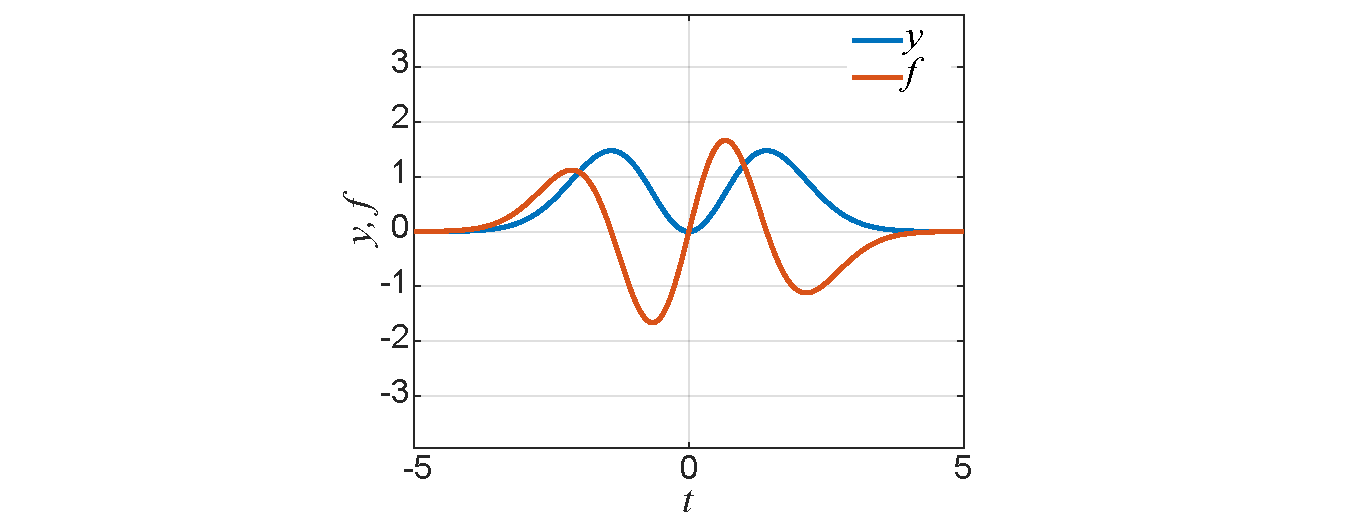
\includegraphics[width=\textwidth]{MatLabSymbolic.pdf}
\caption[Ergebnisfenster des \matlab-Programms f�r symbolische Berechnung.]{Ergebnisfenster des \matlab-Programms f�r eine symbolische Berechnung.}\label{abb:solman_matlab_symb}
\end{figure}

%-----------------------------------------------------------------------------------------------------------------------------------------------------------------------------
\section{Toolboxen}
Auch wenn es aus methodisch-didaktischer Sicht sinnvoll erscheint, sich seine eigenen Funktionsbibliotheken zu erstellen, muss das Rad nicht immer neu erfunden werden.
Die Basis-F�higkeiten von \matlab{} k�nnen n�mlich durch die Verwendung von vorkonfigurierten Toolboxen signifikant erweitert werden. Diese kuratierten Toolboxen m�ssen separat installiert werden. Toolboxen sind Bibliotheken von Skripten, die von der Firma Mathworks und Kooperationspartnern (\url{http://www.mathworks.com}) erstellt wurden, um bestimmte Problemgruppen zu l�sen. Derzeit sind \ua folgende Toolboxen verf�gbar, die f�r die Anwendungen in diesem Buch und in der CP relevant sind:
\begin{itemize}
	\item Symbolic Math Toolbox
	\item Mapping Toolbox
	\item Partial Differential Equation Toolbox
	\item Statistics and Machine Learning Toolbox
	\item Curve Fitting Toolbox
	\item Optimization Toolbox
	\item Image Processing Toolbox
	\item Verschiedene Toolboxen zur Physikalische Modellierung
\end{itemize}
Ausf�hrlichere Informationen zu diesen Toolboxen erhalten Sie unter \url{http://www.mathworks.com}.
Das Kommando \mlcmd{ver} listet zudem alle installierten Toolboxen und deren Versionsnummern auf.

\chapter{Verzeichnis der \mscre} \label{kap:solman_matlablist}

\subsection{\mscre -- Physik der Bewegung}\label{kap:bew_matlabskripts}

Die \mscre befinden sich im MATLAB-Ordner \texttt{MatlabDateien/bew},
die Hilfsfunktionen im dortigen Unterordner \texttt{Include\-folder} und Daten im Unterordner \texttt{Data}.
Es wird empfohlen, entweder die Skripte im GitHub Verzeichnis \githubSN zu benutzen oder sich die komplette Verzeichnisstruktur von \MKc~ runter zu laden und diese und auch das Arbeitsbuch im Hauptverzeichnis Fingeruebungen zu installieren. \\

Wir wollen noch einmal explizit darauf hinweisen, dass die \mscre prim�re der Vermittlung der physikalischen Modelle dienen und keinen Anspruch auf besonders elegante oder effiziente Programmierung erheben. Unser Buch ist ja kein Lehrbuch f�r \matlab-Programmierung. Uns ging es bewusst darum, dass die Skripte gut lesbar sind und das physikalische Modell bzw den physikalischen Gedankengang m�glichst klar abbilden.
Die Leser sind aufgerufen, die Programme nach Belieben zu verbessern und kompakter zu gestalten und diese auch ins GitHub Verzeichnis \githubSN zu stellen.

\subsubsection {Skripte zu Beispielen} \label{mls:bew_kapitel} 
\begin{longtable}{p{0.33\textwidth}p{0.67\textwidth}}
\hline\noalign{\smallskip}
Skript & Beschreibung \\
\noalign{\smallskip}\svhline\noalign{\smallskip}
%\href{bew/matlab/HarmonOszillator.m}{HarmonOszillator.m} & L�sung der Bewegungsgleichung f�r den getriebenen harmonischen Oszillator mit Reibung.\\

%\mlbewref{AchterbahnLoop.m}             & Durchlaufen einer kreisf�rmigen Loop auf einer Achterbahn (Einzelner Wagen und Zug im Vergleich).\\
\mlbewref{AnHarmonOszillator01.m}       & Schwingungsperiode f�r den anharmonischen Oszillator exakt und in verschiedenen N�herungen.\\
\mlbewref{AnHarmonOszillator02.m}       & L�sung der Bewegungsgleichung f�r den anharmonischen Oszillator in verschiedenen N�herungen.\\
\mlbewref{BungeeJumping.m}              & L�sung der Lagrange-Gleichungen f�r das Bungee-Jumping.\\
\mlbewref{Doppelkegel01.m}              & Herleitung der Lagrange-Gleichungen f�r den aufw�rts rollenden Doppelkegel aus der Lagrange-Funktion mittels der symbolischen Toolbox von \matlab.\\
\mlbewref{Doppelkegel02.m}              & L�sung der Lagrange-Gleichungen f�r den aufw�rts rollenden Doppelkegel.\\
\mlbewref{Doppelkegel03.m}              & Phasenraum des aufw�rts rollenden Doppelkegels aus der Energieerhaltung.\\
\mlbewref{Doppelkegel04.m}              & Phasenraum des aufw�rts rollenden Doppelkegels aus der Energieerhaltung f�r verschiedene Parameter.\\
\mlbewref{Doppelpendel01.m}             & Herleitung der Lagrange-Gleichungen f�r das Doppelpendel aus der Lagrange-Funktion mittels der symbolischen Toolbox von \matlab.\\
\mlbewref{Doppelpendel02.m}             & Beispielrechnungen und Simulation des Doppelpendels.\\
\mlbewref{FallendeKette.m}              & L�sung der Lagrange-Gleichungen f�r die fallende Kette.\\
\mlbewref{FallendeLeiter.m}             & Dynamik f�r eine fallende ("`wegrutschende"') Leiter.\\
\mlbewref{FallenderStab01.m}            & Kr�fteverh�ltnisse bei fallenden Stab.\\
\mlbewref{FallenderStab02.m}            & L�sung der Lagrange-Gleichungen f�r den fallenden Stab f�r verschiedene Reibungskoeffizienten.\\
\mlbewref{FoucaultPendel.m}             & Drehung der Schwingungsebene beim Foucault-Pendel.\\
\mlbewref{GekoppeltePendel01.m}         & Beispielrechnungen und Simulation der gekoppelten Pendel f�r gleiche Pendel, kleine Winkel.\\
\mlbewref{GekoppeltePendel02.m}         & Beispielrechnungen und Simulation der gekoppelten Pendel f�r unterschiedliche Pendel, kleine Winkel.\\
\mlbewref{GekoppeltePendel03.m}         & Beispielrechnungen und Simulation der gekoppelten Pendel f�r allgemeine Bedingungen, gro�e Winkel.\\
\mlbewref{Gyrotwister.m}                & Simulation der Beschleunigung des Kreisels im Gyrotwister durch die Bewegung der Hand.\\
\mlbewref{GyrotwisterPhase.m}           & Simulation der Beschleunigung des Kreisels im Gyrotwister durch die Bewegung der Hand bei einer Phasendifferenz zur optimalen Bewegung.\\
\mlbewref{HarmonOszillator.m}           & L�sung der Bewegungsgleichung f�r den getriebenen harmonischen Oszillator mit Reibung.\\
\mlbewref{Harpune.m}                    & L�sung der Lagrange-Gleichungen f�r einen senkrecht geworfenen Enterhaken/eine Harpune.\\
\mlbewref{JoJo01.m}                     & Berechnungen zur Dynamik eines Jo-Jos.\\
\mlbewref{KfKreiselFreieAchsen.m}       & Beispielrechnungen und Simulation zur Stabilit�t des kr�ftefreien Kreisels mit freien Achsen.\\
\mlbewref{KfSymmKreiselNutation.m}      & Beispielrechnungen zur Nutation des kr�ftefreien symmetrischen Kreisels im raumfesten System.\\
\mlbewref{Klothoide.m}                  & Berechnungen zur Klothoide (Cornu-Spirale) und Form eines Loopings f�r eine Achterbahn.\\
\mlbewref{KopPendelKleinWinkel.m}       & Beispielrechnungen und Simulation der gekoppelten Pendel f�r die Kleinwinklen�herung (analytische und numerische Rechnung).\\
\mlbewref{NLOszillator01.m}             & L�sung der Bewegungsgleichung f�r den getriebenen nichtlinearen Oszillator mit Reibung.\\
\mlbewref{NLOszillator02.m}             & Berechnung des Ljapunow-Exponenten f�r den getriebenen nichtlinearen Oszillator mit Reibung.\\
\mlbewref{Pendeluhr.m}                  & Berechnungen zur Pendeluhr.\\
\mlbewref{RollendesRad.m}               & Bewegung eines rollenden Rades.\\
\mlbewref{Rutherford.m}                 & Berechnungen zur Rutherford-Streuung.\\
\mlbewref{Schaukel01.m}                 & Berechnungen zur Dynamik einer Schaukel als parametrischen Oszillator.\\
\mlbewref{Schaukel02.m}                 & Berechnungen zur Dynamik einer Schaukel als getriebener Oszillator H�he.\\
\mlbewref{SchwererKreiselPraez01.m}     & Simulationsrechnung zur Pr�zession des schweren symmetrischen Kreisels im raumfesten System.\\
\mlbewref{SchwererKreiselPraez02.m}     & Beispielrechnungen zur Pr�zession des schweren symmetrischen Kreisels im raumfesten System.\\
\mlbewref{TrebSimDAE.m}                 & Berechnungen zur Dynamik eines \textit{Trebuchet}. Trebuchet mit Ber�cksichtigung von Zwangsbedingungen.\\
\mlbewref{TrebuchetSim02.m}             & Berechnungen zur Dynamik eines \textit{Trebuchet}. Modelle ohne Ber�cksichtigung der Zwangsbedingungen.\\
\mlbewref{TrebuchetLGL02.m}             & Symbolische Berechnung Lagrange-Funktion und Lagrange-Gleichungen f�r ein \textit{Trebuchet}.\\

\noalign{\smallskip}\svhline\noalign{\smallskip}
\end{longtable}

\newpage
\subsubsection{Skripte zu �bungen} \label{mls:bew_uebungen} %MLSkript�bungen
\begin{longtable}{p{0.33\textwidth}p{0.67\textwidth}}
\hline\noalign{\smallskip}
Skript & Beschreibung \\
\noalign{\smallskip}\svhline\noalign{\smallskip}
\mlbewref{AbplattungPlaneten.m}      & Berechnungen zur Abplattung der Planeten.\\
\mlbewref{Achterbahn01.m}            & Zeitliche Entwicklung eines Massepunktes auf einer Gau�-Kurve ($z = H\e^{-a^2 x^2}$) unter Einfluss der Gravitation.\\
\mlbewref{Achterbahn02.m}            & Zeitliche Entwicklung eines Massepunktes auf einer vorgegebenen Kurve ($z = 1+\tanh(x)$) unter Einfluss der Gravitation.\\
\mlbewref{Achterbahn03.m}            & Zeitliche Entwicklung der Bewegung eines Massepunktes auf einer parametrisierten Kurve (Trisectrix) unter Einfluss der Gravitation.\\
\mlbewref{Achterbahn04.m}            & Zug $N$ mit Federn gekoppelter Wagen auf einer Achterbahn in Form einer Gau�-Kurve.\\
\mlbewref{Achterbahn06.m}            & Zug $N$ mit Federn gekoppelter Wagen auf einer Achterbahn in Form eines Kreisloopings.\\
\mlbewref{AsteroidKollision.m}       & Kollisionswahrscheinlichkeit von Asteroiden mit Planeten.\\
\mlbewref{AsteroidStreuung.m}        & Berechnung von Trajektorien f�r Asteroiden in der Erdbahn.\\
\mlbewref{AsymmKreiselStab.m}        & Betrachtung zur Stabilit�t des asymmetrischen Kreisels, numerische L�sungen mittels \odevf.\\
\mlbewref{BallistikCoriolis01.m}     & Berechnung der Effekte der Coriolis-Kraft auf den freien Fall.\\
\mlbewref{BallistikCoriolis02.m}     & Berechnung der Effekte der Coriolis-Kraft auf die Ballistik eines Projektils, das nach S�den abgeschossen wird. Exakte L�sung.\\
\mlbewref{BallistikCoriolis03.m}     & Berechnung der Effekte der Coriolis-Kraft auf die Ballistik eines Projektils, das nach S�den abgeschossen wird. Die Reibung wird ber�cksichtigt. Numerische L�sung mittels \odevf.\\
\mlbewref{Baton.m}                   & Bewegungsgleichung Baton, numerische L�sung mittels \odevf. \\
\mlbewref{BaumgartnerFall.m}         & Freier Fall aus gro�er H�he (Baumgartner-Weltrekord).\\
\mlbewref{Billardspiel.m}            & Berechnung der Streuwinkel und Geschwindigkeiten beim Sto� zweier Billardkugeln.\\
\mlbewref{Brachistochrone.m}         & Berechnungen zur Brachistochrone und Tautochrone, sowie Lagrange-Funktion und  Lagrange Gleichungen des Zykloidenpendels.\\
\mlbewref{Doppelkegel05.m}           & Phasenraum und Dynamik des aufw�rts rollenden Doppelkegels (N�herung 1).\\
\mlbewref{Doppelkegel06.m}           & Phasenraum und Dynamik des aufw�rts rollenden Doppelkegels (N�herung 2).\\
\mlbewref{DoppelkegelVergleich.m}    & Vergleich der L�sungen f�r den aufw�rts rollenden Doppelkegel.\\
\mlbewref{ElastischerStoss.m}        & Berechnung des Energie�bertrag als Funktion des Streuwinkels im Laborsystem.\\
\mlbewref{EulerWinkel.m}             & Berechnung von Euler-Winkeln.\\
\mlbewref{Expander.m}                & Abh�ngigkeit der Schwingungsperiode von der Anfangsauslenkung eines intrinsisch nichtlinearen Oszillators am Beispiel eine Expanders.\\
\mlbewref{Gezeitenkraefte.m}         & Berechnet die Verformung eines Rings durch Gezeitenkr�fte.\\
\mlbewref{GekoppeltePendel01.m}      & L�sung der Bewegungsgleichung analytisch und numerisch f�r gekoppelte Stangenpendel (kleine Winkel, gleiche L�ngen). \\
\mlbewref{GekoppeltePendel02.m}      & L�sung der Bewegungsgleichung analytisch und numerisch f�r gekoppelte Stangenpendel (kleine Winkel, unterschiedliche L�ngen). \\
\mlbewref{GekoppeltePendel03.m}      & L�sung der Bewegungsgleichung mit/ohne Reibung f�r gekoppelte Stangenpendel (allgemeiner Fall). \\
\mlbewref{Hantelwurf.m}              & Berechnung der Bahn einer geworfenen Hantel als numerische L�sung mittels \odevf.\\
\mlbewref{HarmonOszQuadReibung.m}    & L�sung der Bewegungsgleichung f�r den harmonischen Oszillator mit Newton-Reibung.\\
\mlbewref{JoJo02.m}                  & Berechnungen zur Dynamik eine angetrieben Jo-Jos mit Reibung.\\
\mlbewref{KarussellCoriolis01.m}     & Berechnung der Effekte der Coriolis-Kraft auf einem gleichf�rmig rotierenden Karussell.\\
\mlbewref{KarussellCoriolis02.m}     & Berechnung der Effekte der Coriolis-Kraft auf einem beschleunigt rotierenden Karussell.\\
\mlbewref{Kettenfontaene.m}          & Programm berechnet den Z-Verlauf der Kettenfont�ne.\\
\mlbewref{KfSymmKreiselSimul.m}      & Simulationsrechnung der Nutation des kr�ftefreien symmetrischen Kreisels.\\
\mlbewref{KfKreiselDrehimpuls.m}     & Beispiele zur Simulation des allgemeinen kr�ftefreien Kreisels und seines Drehimpulses im k�rperfesten System.\\
\mlbewref{Kontraktion.m}             & Berechnungen zur Kontraktion und Energie einer rotierenden Galaxie.\\
\mlbewref{KopPendelKleinWinkel.m}    & Dynamik der gekoppelten Federpendel.\\
\mlbewref{KreiselKomp.m}             & Simulation des Einstellens der Nordrichtung beim fl�ssigkeitsged�mpften Kreiselkompass.\\
\mlbewref{KreiselKompMissweisung.m}  & Berechnung der Missweisung eines Kreiselkompasses bei Bewegung entlang eines L�ngenkreises.\\
\mlbewref{LagrangePunkte.m}          & Berechnung der Hill-Kurve und der Lagrange-Punkte.\\
\mlbewref{LogistischeGleichung01.m}  & Berechnung der Trajektorien der Logistischen Gleichung.\\
\mlbewref{LogistischeGleichung02.m}  & Bifurkationsgraph und Ljapunow-Exponent der Logistischen Gleichung.\\
\mlbewref{MolekuelPot.m}             & Simulation der Schwingungen eines zweiatomigen Molek�ls.\\
\mlbewref{MurphysLaw.m}              & Simulation zu Murphy's Law (Butterbrotscheiben-Versuch).\\
\mlbewref{PerleDraht.m}              & L�sung der Bewegungsgleichung ohne Reibung f�r die Perle auf Draht. \\
\mlbewref{PerleDrahtErweiterung.m}   & L�sung der Bewegungsgleichung mit Reibung f�r die Perle auf Draht mit verschiedenen Potentialen. \\
\mlbewref{Rollenpendel.m}            & L�sung der Bewegungsgleichung ohne Reibung f�r das Rollenpendel. \\
\mlbewref{RollenpendelReibung.m}     & L�sung der Bewegungsgleichung mit Reibung f�r das Rollenpendel.\\
\mlbewref{RollendesRad.m}            & Berechnung der Euler-Winkel und der Trajektorie einer Kreisscheibe \bzw eines Reifens auf einer ebenen Fl�che (ohne Reibung).\\
\mlbewref{RollendesRadR.m}           & Berechnung der Euler-Winkel und der Trajektorie einer Kreisscheibe \bzw eines Reifens auf einer ebenen Fl�che (mit Reibung).\\
\mlbewref{RutherfordAlpha.m}         & Trajektorienberechnung der Rutherford-Streuung von $\alpha$-Teilchen an Goldfolie.\\
\mlbewref{RutherfordAg.m}            & Trajektorienberechnung der Rutherford-Streuung von Silber-Teilchen an Goldfolie.\\
\mlbewref{SchaukelLG.m}              & Lagrange-Gleichung f�r die Schaukel mit sitzender und schwingender Person.\\
\mlbewref{Schaukel03.m}              & L�sung der DGL f�r die Schaukel mit Kette und verhindertem �berschlag.\\
\mlbewref{SchwererKreiselSim.m}      & Simulation der Figurenachse eines schweren Kreisels mit und ohne Nutation.\\
\mlbewref{Sinuslauf.m}               & Berechnung der Frequenz und Stabilit�t des Sinuslaufs bei starren Radachsen auf Schienen.\\
\mlbewref{Skydiver.m}                & Berechnung Fall aus gro�er H�he (Baumgartner-Weltrekord).\\
\mlbewref{SwingBy.m}                 & Berechnungen zum Swing- By am Jupiter.\\
\mlbewref{Tilgung01.m}               & Berechnung der Schwingungsd�mpfung in Hochh�usern.\\
\mlbewref{Tilgung02.m}               & Programm berechnet Frequenzantwort bei der Schwingungsd�mpfung an Hochh�usern.\\
\mlbewref{Tilgung03.m}               & Programm berechnet Frequenzantwort Schwingungsd�mpfung f�r Taipei 101 und den Berliner Fernsehturm.\\
\mlbewref{Traegheitsmomente.m}       & Berechnungen zu Tr�gheitsmomenten.\\
\mlbewref{TrebuchetLGL01.m}          & Lagrange-Funktion und Lagrange-Gleichungen f�r ein \textit{Trebuchet}.\\
\mlbewref{TrebuchetSim01.m}          & Berechnungen zur Dynamik des \textit{Trebuchet}.\\
\mlbewref{VibDaempfung01.m}          & Berechnung der Dynamik eines Sto�d�mpfers auf Basis Lagrange-Gleichungen.\\
\mlbewref{VibDaempfung02.m}          & Berechnung der D�mpfung einer Deckenaufh�ngung.\\
\mlbewref{Waschmaschine01.m}         & Berechnung des Schwingungs- und Resonanzverhaltens einer Trommelwaschmaschine in der Hochlaufphase.\\
\mlbewref{Waschmaschine02.m}         & Berechnung des Schwingungs- und Resonanzverhaltens einer Trommelwaschmaschine in der Auslaufphase.\\
\mlbewref{WeltraumFahrstuhl.m}       & Berechnungen zum Weltraumfahrstuhl.\\
\mlbewref{Wilberforce.m}             & Berechnung der Dynamik des linearen und nichtlinearen Wilberforce-Pendels auf Basis von Lagrange-Gleichungen (Resonanzfall).\\
\mlbewref{WurfmitohneReibung.m}      & Berechnung Auf- und Abstiegszeiten beim senkrechten Wurf mit und ohne Reibung.\\

\noalign{\smallskip}\hline\noalign{\smallskip}
\end{longtable}


\subsubsection {Hilfsfunktionen} \label{mls:bew_hilfsfunktionen} 

\begin{longtable}{p{0.33\textwidth}p{0.67\textwidth}}
\hline\noalign{\smallskip}
Skript & Beschreibung \\
\noalign{\smallskip}\svhline\noalign{\smallskip}
Mathematische Funktionen \\
\noalign{\smallskip}\svhline\noalign{\smallskip}
\mlbewiref{EulerLagrange.m}             & Symbolische Berechnung der Euler-Lagrange Gleichungen (\url{https://www.mathworks.com/matlabcentral/fileexchange/93275-euler-lagrange-solver}), MATLAB Central File Exchange. 27.12.2021, Copyright (c)  Morten Veng 2021.\\
\mlbewiref{Modulo.m}                    & Modulus-Funktion.\\
\mlbewiref{R\_x.m}, \mlbewiref{R\_y.m}, \mlbewiref{R\_z.m}     & Rotationsmatrizen bez�glich x,y,z-Achse.\\

\noalign{\smallskip}\svhline\noalign{\smallskip}
Hilfsfunktionen f�r Ein- und Ausgabe \\
\noalign{\smallskip}\svhline\noalign{\smallskip}
\mlbewiref{Ausgabewerte.m}              & Printfunktion f�r Ausgabewerte.\\
\mlbewiref{GetColorLines.m}             & L�dt Farbtabelle f�r Linien und graphische Darstellungen.\\
\mlbewiref{ImportFile01.m}              & Einlesen von Daten einer Matrix.\\ 
\mlbewiref{ImportFile02.m}              & Einlesen von Daten eines Text-Files.\\
\mlbewiref{LabelPoints.m}               & Beschriftung von Datenpunkten.\\
\mlbewiref{PlotCircle.m}	            & Graphische Ausgabe von Fr�hlingspunkt und Sonnen.\\
\mlbewiref{PlotTrebuchet.m}	            & Graphische Ausgabe der Geometrie eines Trebuchet.\\
\mlbewiref{StrDMS.m}                    & Umrechnung von Formaten f�r Ausgabe von Winkeln von Dezimal in Grad, Bogenminute, Bogensekunde.\\
\mlbewiref{StrHMS.m}                    & Umrechnung von Formaten f�r Ausgabe von Zeit von Dezimal in hh:mm:ss.s.\\
\noalign{\smallskip}\svhline\noalign{\smallskip}
\end{longtable}


 
\clearpage
\subsection{\mscre -- Physik des Kontinuums}\label{kap:kontmech_matlabskripts}

Die \mscre befinden sich im MATLAB-Ordner \texttt{MatlabDateien/kontmech},
die Hilfsfunktionen im dortigen Unterordner \texttt{Include\-folder} und Daten im Unterordner \texttt{Data}.
Es wird empfohlen, entweder die Skripte im GitHub Verzeichnis \githubSN zu benutzen oder sich die komplette Verzeichnisstruktur von \MKc~ runter zu laden und diese und auch das Arbeitsbuch im Hauptverzeichnis Fingeruebungen zu installieren. \\

Wir wollen noch einmal explizit darauf hinweisen, dass die \mscre prim�re der Vermittlung der physikalischen Modelle dienen und keinen Anspruch auf besonders elegante oder effiziente Programmierung erheben. Unser Buch ist ja kein Lehrbuch f�r \matlab-Programmierung. Uns ging es bewusst darum, dass die Skripte gut lesbar sind und das physikalische Modell bzw den physikalischen Gedankengang m�glichst klar abbilden.
Die Leser sind aufgerufen, die Programme nach Belieben zu verbessern und kompakter zu gestalten und diese auch ins GitHub Verzeichnis \githubSN zu stellen.


%\begin{prob}\label{mls:kontmech_hilfsfunktionen} %MLSkript1 
%\textbf{Hilfsfunktionen} \\
%\begin{longtable}{p{0.33\textwidth}p{0.67\textwidth}}
%\hline\noalign{\smallskip}
%Skript & Beschreibung \\
%\noalign{\smallskip}\svhline\noalign{\smallskip}
%Mathematische Funktionen \\
%\noalign{\smallskip}\svhline\noalign{\smallskip}
%\mlkontmechref{Beispiel.m} & Ein Beispieltext.\\
%\noalign{\smallskip}\svhline\noalign{\smallskip}
%\end{longtable}
%\end{prob}

\subsubsection {Skripte zu Beispielen} \label{mls:kontmech_kapitel} 
\begin{longtable}{p{0.33\textwidth}p{0.67\textwidth}}
\hline\noalign{\smallskip}
Skript & Beschreibung \\
\noalign{\smallskip}\svhline\noalign{\smallskip}
\mlkontmechref{SchwingendeSaite01.m} & L�sen der Differentialgleichung einer
schwingenden Saite f�r eine stehende Welle.\\
\noalign{\smallskip}\svhline\noalign{\smallskip}
\end{longtable}

\subsubsection {Skripte zu �bungen} \label{mls:kontmech_uebungen} 
\begin{longtable}{p{0.33\textwidth}p{0.67\textwidth}}
\hline\noalign{\smallskip}
Skript & Beschreibung \\
\noalign{\smallskip}\svhline\noalign{\smallskip}
\mlkontmechref{AchterbahnKont.m}        & L�sen der Differentialgleichung eines kontinuierlichen, elastischen Achterbahnzuges auf einer Gau�kurven-Strecke.\\
\mlkontmechref{AchterbahnKontBeschl.m}  & Normalbeschleunigung auf einen Fahrgast im kontinuierlichen, elastischen Achterbahnzug.\\
\mlkontmechref{Chladni01.m}             & L�sen der Eigenschwingungen einer kreisf�rmigen, elastischen Fl�che.\\
\mlkontmechref{Chladni02.m}             & L�sen der Eigenschwingungen einer quadratischen, elastischen Fl�che.\\
\mlkontmechref{Chladni03.m}             & L�sen der Eigenschwingungen einer rechteckigen, elastischen Fl�che.\\
\mlkontmechref{Divergenz.m}             & Programm berechnet Vektorfunktionen und ihre Divergenz.\\
\mlkontmechref{FassFormelGauss.m}       & Programm berechnet Volumen von Rotationsk�rpern �ber Gau�schen Integralsatz.\\
\mlkontmechref{GespannterBogen.m}       & L�sen der Eigenschwingungen eines Bogens, der durch eine Saite gespannt ist.\\
\mlkontmechref{GradientFunktion1.m}     & Programm berechnet Funktionen und ihre Gradienten.\\
\mlkontmechref{GradientFunktion2.m}     & Programm berechnet Funktionen und ihre Gradienten (Yukawa-Potential).\\
\mlkontmechref{GradientFunktion3.m}     & Programm berechnet Funktionen und ihre Gradienten (Kepler-Potential mit Drehimpuls).\\
\mlkontmechref{KdVTsunami.m}            & Berechnung eines KdV-Solitons, das auf eine K�ste zul�uft, an der die Wassertiefe abnimmt.\\
\mlkontmechref{KdV01.m}                 & L�sen der Korteweg-de-Vries-Gleichung f�r ein einzelnes Soliton.\\
\mlkontmechref{KdV02.m}                 & Vergleich mehrerer Solitonen der KdV-Gleichung mit unterschiedlicher Geschwindigkeit.\\
\mlkontmechref{KdV03.m}                 & Summen aus einzelnen Solitonen in der KdV-Gleichung.\\
\mlkontmechref{KdV04.m}                 & Interaktion von Solitonen in der KdV-Gleichung.\\
\mlkontmechref{Kreisrohr.m}             & Berechnen des Geschwindigkeitsprofils einer station�ren Str�mung in einem kreisrunden Rohr.\\
\mlkontmechref{NLSGSolitonen.m}         & L�sen der nichtlinearen Schr�dinger-Gleichung f�r ein Soliton.\\
\mlkontmechref{Rechteckrohr.m}          & Berechnen des Geschwindigkeitsprofils einer station�ren Str�mung in einem rechteckigen Rohr.\\
\mlkontmechref{Rotation.m}              & Programm berechnet Vektorfunktionen und ihre Rotation.\\
\mlkontmechref{SchwingendeSaite02.m}    & L�sen der Differentialgleichung einer eingespannten Saite f�r eine Gau�sche St�rung.\\
\mlkontmechref{SchwingendeSaite03.m}    & L�sen der Differentialgleichung einer eingespannten Saite f�r eine einseitig angeregte Welle.\\
%\noalign{\smallskip}\svhline\noalign{\smallskip}
\mlkontmechref{SinusGordonSolitonen.m}  & L�sen der Sinus-Gordon-Gleichung f�r ein Soliton.\\
\mlkontmechref{Tank.m}  & Fluss durch einen quadratischen Tank mit zwei �ffnungen.\\
\mlkontmechref{Torricelli.m}  & Fluss einer Fl�ssigkeit aus einem Tank nach dem
Gesetz von Torricelli.\\
\end{longtable}



 
\clearpage
\subsection{\mscre--Himmelsmechanik}\label{kap:hm_matlabskripts}

Die \mscre befinden sich im MATLAB-Ordner \texttt{MatlabDateien/hm},
die Hilfsfunktionen im dortigen Unterordner \texttt{Include\-folder} und Daten im Unterordner \texttt{Data}.

Die \mscre befinden sich im MATLAB-Ordner \texttt{MatlabDateien/hm},
die Hilfsfunktionen im dortigen Unterordner \texttt{Include\-folder} und Daten im Unterordner \texttt{Data}.
Es wird empfohlen, entweder die Skripte im GitHub Verzeichnis \githubSN zu benutzen oder sich die komplette Verzeichnisstruktur von \MKc~ runter zu laden und diese und auch das Arbeitsbuch im Hauptverzeichnis Fingeruebungen zu installieren. \\

Wir wollen noch einmal explizit darauf hinweisen, dass die \mscre prim�re der Vermittlung der physikalischen Modelle dienen und keinen Anspruch auf besonders elegante oder effiziente Programmierung erheben. Unser Buch ist ja kein Lehrbuch f�r \matlab-Programmierung. Uns ging es bewusst darum, dass die Skripte gut lesbar sind und das physikalische Modell bzw den physikalischen Gedankengang m�glichst klar abbilden.
Die Leser sind aufgerufen, die Programme nach Belieben zu verbessern und kompakter zu gestalten und diese auch ins GitHub Verzeichnis \githubSN zu stellen.

\subsubsection{Skripte zu Beispielen}\label{mls:hm_bsp_uebungen} %MLSkript1 

\subparagraph{\textbf{Exzentrizit�t Planetenbahnen}}\label{mls:hm_exzentri} %MLSkript2
\begin{longtable}{p{0.33\textwidth}p{0.67\textwidth}}
\hline\noalign{\smallskip}
Skript & Beschreibung \\
\noalign{\smallskip}\svhline\noalign{\smallskip}
\mlhmref{PlanetExzentrizitaeten.m}	& Darstellung der Exzentrizit�ten der Planetenbahnen (auf gro�e Halbachse $a$ normiert).\\
\noalign{\smallskip}\hline\noalign{\smallskip}
\end{longtable}

\subparagraph{\textbf{Analemma}}\label{mls:hm_analemma} %MLSkript3
\begin{longtable}{p{0.33\textwidth}p{0.67\textwidth}}
\hline\noalign{\smallskip}
Skript & Beschreibung \\
\noalign{\smallskip}\svhline\noalign{\smallskip}
\mlhmref{Analemma01.m}        & Analemma auf Basis einer auf der Mittelpunktsgleichung basierenden Keplerl�sung f�r die Sonnenbahn. Exzentrizit�t und Ekliptikschiefe werden variiert (�quinoktium und Ekliptik des Datums). \\
\mlhmref{Analemma02.m}        & Analemmaberechnung (N�herungsrechnung) f�r verschiedene geographische Positionen in Alt-Azimut-Darstellung f�r 24 h. Refraktion und Tagbogenverl�ngerung vernachl�ssigt. Es wird eine einfache auf der Mittelpunktsgleichung basierenden Keplerl�sung f�r die Erdbahn benutzt (�quinoktium und Ekliptik des Datums). \\
\mlhmref{Analemma03.m}        & Analemmaberechnung f�r verschiedene Planeten direkt aus der exzentrischen Anomalie $E$ ohne L�sung der Kepler-Gleichung.\\
\mlhmref{AnalemmaSonne.m}  & Analemmaberechnung der Sonne vom Mond aus auf Basis von auf der Mittelpunktsgleichung basierenden Keplerl�sungen f�r die Sonnen- und Mondbahn.\\
\mlhmref{AnalemmaMond.m}    & Analemmaberechnung f�r Mond von der Erde aus betrachtet auf Basis von auf der Mittelpunktsgleichung basierenden Keplerl�sungen f�r die Sonnen- und Mondbahn.\\
\mlhmref{AnalemmaOkoFit.m}    & Umrechnung einschlie�lich Bildkorrektur des aufgenommenen Analemma von Oberkochen 2019/20 in das horizontale KOS, sowie Darstellung verschiedener theoretisch berechneter Analemma. \\
\mlhmref{AnalemmaFindExz.m}   & Umrechnung einschlie�lich Bildkorrektur des aufgenommenen Analemma von Oberkochen 2019/20 in das horizontale KOS, sowie Fit eines theoretisch berechneten Analemmas mit der Exzentrizit�t e als Parameter. \\
\noalign{\smallskip}\hline\noalign{\smallskip}
\end{longtable}

\subparagraph{\textbf{Sonnenaufgangsberechnung (Methode der quadratischen Interpolation)}}\label{mls:hm_sonnenaufgang} %MLSkript4
\begin{longtable}{p{0.33\textwidth}p{0.67\textwidth}}
\hline\noalign{\smallskip}
Skript & Beschreibung \\
\noalign{\smallskip}\svhline\noalign{\smallskip}
\mlhmref{Sonnenaufgang01.m} & Aufgangs- und Untergangszeiten der Sonne f�r verschiedene geographische Orte (Breite < 60�) und die Tagl�ngen
 iterativ aus der Kepler-Gleichung f�r das ganze Jahr und in der N�he des Jahreswechsels bzw. Mitsommers.\\
\mlhmref{Sonnenaufgang02.m} & Aufgangszeiten auf Basis der Kepler-Gleichung  a) mit einer iterativen Methode (Quadratische 
Interpolation) zur Suche der Nullstellen f�r Auf- und Unterg�nge und b) zum Vergleich auf Basis der ZGL-N�herung.\\
\noalign{\smallskip}\hline\noalign{\smallskip}
\end{longtable}

\subparagraph{\textbf{Vergleich Zeitgleichung}}\label{mls:hm_zeitglgformeln} %MLSkript5
\begin{longtable}{p{0.33\textwidth}p{0.67\textwidth}}
\hline\noalign{\smallskip}
Skript & Beschreibung \\
\noalign{\smallskip}\svhline\noalign{\smallskip}
\mlhmref{ZGL01.m} & ZGL auf Basis einer Mittelpunktsgleichung basierenden Keplerl�sung f�r die Sonnenbahn und Vergleich mit empirischen Werten und den Berechnungen des JPL (�quinoktium und Ekliptik des Datums). \\
\mlhmref{ZGL02.m} & Reihenentwicklung der ZGL.\\
\mlhmref{ZGL03.m} & ZGL auf Basis einer (auf der Mittelpunktsgleichung basierten) Keplerl�sung f�r die Erdbahn und Vergleich mit verschiedenen publizierten N�herungsformeln und den Berechnungen des JPL. \\
\noalign{\smallskip}\hline\noalign{\smallskip}
\end{longtable}
 
\subparagraph{\textbf{Tagbogen-Verl�ngerung}}\label{mls:hm_tagbogenverl} %MLSkript6
\begin{longtable}{p{0.33\textwidth}p{0.67\textwidth}}
\hline\noalign{\smallskip}
Skript & Beschreibung \\
\noalign{\smallskip}\svhline\noalign{\smallskip}
\mlhmref{TagbogenVerlaengerung.m} & Tagbogenverl�ngerung bedingt durch Refraktion und scheinbaren Sonnendurchmesser bei Sonnenaufgang.\\
\noalign{\smallskip}\hline\noalign{\smallskip}
\end{longtable}

%\newpage
\subparagraph{\textbf{Tageslauf Sonne}}\label{mls:hm_tageslauf_sonne} %MLSkript7
\begin{longtable}{p{0.33\textwidth}p{0.67\textwidth}}
\hline\noalign{\smallskip}
Skript & Beschreibung \\
\noalign{\smallskip}\svhline\noalign{\smallskip}
\mlhmref{TageslaufSonne01.m} & Der Tageslauf der Sonne wird nach der N�herungsformel (3.84) berechnet. Die geographische Breite kann variiert werden. Es wird die H�he der Sonne f�r verschieden Jahreszeiten und geographische Breiten dargestellt. Die ZGL wird nicht ber�cksichtigt.
Berechnung des Tagbogenverlaufs (N�herung) der Sonne �ber dem Horizont f�r verschiedene Jahreszeiten und geographische Breiten.\\
\mlhmref{TageslaufSonne02.m} & Tagbogenverlauf der Sonne �ber dem Horizont. (N�herungsformel und zum numerische L�sung. Die geographische Breite kann variiert werden.\\
\noalign{\smallskip}\hline\noalign{\smallskip}
\end{longtable}
 


\subparagraph{\textbf{Berechnung der Aufgangswinkel der Sonne (Verschiedene Orte und Jahreszeiten)}}\label{mls:hm_aufgangswinkel_sonne} %MLSkript8
\begin{longtable}{p{0.33\textwidth}p{0.67\textwidth}}
\hline\noalign{\smallskip}
Skript & Beschreibung \\
\noalign{\smallskip}\svhline\noalign{\smallskip}
\mlhmref{SonnenaufgangZeit.m}    & H�he $h$ und Azimut $\mathcal{A}$ und die Zeit-H�hen-Kurven beim Sonnenaufgang auf Basis einer MPG-Keplerl�sung f�r verschiedene geographische Breiten und verschiedene Jahreszeiten (Wintersonnenwende, Fr�hlingsanfang, Sommersonnenwende, Herbstanfang). Dabei wird die astrometrische H�he $h$ und die durch Refraktion \ua Effekte bedingte \anf{scheinbare} H�he $h'$ berechnet.\\ 
\mlhmref{SonnenaufgangBaabe.m}        & H�he $h$ und Azimut $\mathcal{A}$ und die Zeit-H�hen-Kurven beim Sonnenaufgang auf Basis einer MPG-Keplerl�sung f�r die Erdbahn f�r Baabe (Ostsee). Dabei wird die astrometrische H�he $h$ und die durch Refraktion \ua Effekte bedingte \anf{scheinbare} H�he $h'$ berechnet.\\
\noalign{\smallskip}\hline\noalign{\smallskip}
\end{longtable}
 

\subparagraph{\textbf{Innere Planetenbahnen}}\label{mls:hm_innere_planeten} %MLSkript9
\begin{longtable}{p{0.33\textwidth}p{0.67\textwidth}}
\hline\noalign{\smallskip}
Skript & Beschreibung \\
\noalign{\smallskip}\svhline\noalign{\smallskip}
\mlhmref{InnerePlaneten.m} & Bahnen der inneren Planeten auf Basis der Kepler-Geichung. 
(�quinoktium und Ekliptik des Datums) \\
\mlhmref{VenusTransit01.m} & Koordinaten der Venus und des Merkurs bei Transits. Die Zeiten m�ssen n�herungsweise z.\,B. aus \mlhmref{InnerePlaneten.m} bekannt sein. Die Daten werden mit JPL-Daten verglichen. \\
\mlhmref{VenusTransit02.m} & Bestimmung der Astronomischen Einheit aus den Daten eines Venustransits. a) Parallaxen-Methode nach Halley: Die beobachteten Werte f�r zwei geographische Orte zu einer Zeit UT werden dem Internet entnommen, daraus wird die Parallaxe bestimmt und daraus dann die AE berechnet.  b) Kontaktzeitmethode durch Beobachtung an einem Standort.\\
\noalign{\smallskip}\hline\noalign{\smallskip}
\end{longtable}

\subparagraph{\textbf{�u�ere Planetenbahnen}}\label{mls:hm_aussere_planeten} %MLSkript10
\begin{longtable}{p{0.33\textwidth}p{0.67\textwidth}}
\hline\noalign{\smallskip}
Skript & Beschreibung \\
\noalign{\smallskip}\svhline\noalign{\smallskip}
\mlhmref{AeusserePlaneten.m} & Bahnen der �u�eren Planeten auf Basis der Kepler-Gleichung f�r den Zeitraum 1920--2020. (�quinoktium und Ekliptik des Datums) \\
\noalign{\smallskip}\hline\noalign{\smallskip}
\end{longtable}
 
\subparagraph{\textbf{St�rungsrechnung }}\label{mls:hm_stoerunsgrechnung_planeten} %MLSkript11
\begin{longtable}{p{0.33\textwidth}p{0.67\textwidth}}
\hline\noalign{\smallskip}
Skript & Beschreibung \\
\noalign{\smallskip}\svhline\noalign{\smallskip}
\mlhmiref{VenusExakt.m} & Ekliptikale Koordinaten der Venus auf Basis einer Reihenentwicklung \cite{Montenbruck1999}. \\
\mlhmiref{MarsExakt.m} & Ekliptikale Koordinaten des Mars auf Basis einer Reihenentwicklung \cite{Montenbruck1999}. \\
\mlhmiref{JupiterExakt.m} & Ekliptikale Koordinaten des Jupiters auf Basis einer Reihenentwicklung \cite{Montenbruck1999}. \\
\mlhmiref{SonneExakt.m}  & Ekliptikale Koordinaten der Sonne auf Basis der Newcombschen Theorie \cite{Montenbruck1999}. \\
\mlhmiref{MondExakt.m}. & Geozentrisch-�quatoriale Koordinaten des Mondes auf Basis der Brownschen Theorie \cite{Montenbruck1999}. \\
\mlhmref{SL9numerisch.m} & Bahn des Kometen Shoemaker-Levy 9 bis zu seinem Zusammenprall mit dem Jupiter �ber numerische Integration.
\end{longtable}


\subparagraph{\textbf{Periheldrehung des Merkurs}}\label{mls:hm_perihel_merkur} %MLSkript12
\begin{longtable}{p{0.33\textwidth}p{0.67\textwidth}}
\hline\noalign{\smallskip}
Skript & Beschreibung \\
\noalign{\smallskip}\svhline\noalign{\smallskip}
\mlhmref{PerihelKappa2.m}    & Perihel-Verschiebung f�r ein Potential mit Term $\kappa_2 \neq 0$. \\
\mlhmref{PerihelKappa3.m}    & Perihel-Verschiebung f�r ein Potential mit Term $\kappa_3 \neq 0$. \\
\mlhmref{StoerpotentialMerkur.m}  & St�rpotentiale und Gravitationskr�fte der anderen Planeten auf den Merkur als Ursache der Perihel-Verschiebung des Merkurs nach der Newtonschen Mechanik. \\
\noalign{\smallskip}\hline\noalign{\smallskip}
\end{longtable}

\subparagraph{\textbf{Kometenbahnen}}\label{mls:hm_kometenbahnen} %MLSkript13
\begin{longtable}{p{0.33\textwidth}p{0.67\textwidth}}
\hline\noalign{\smallskip}
Skript & Beschreibung \\
\noalign{\smallskip}\svhline\noalign{\smallskip}
\mlhmref{AsteroidenBahnen.m}   & Bahnen der Asteroiden in heliozentrischen Koordinaten unter Benutzung der Gau�schen Vektoren (�quinoktium und Ekliptik des Datums). \\
\mlhmref{AsteroidenZeit.m}     & Bahn eines Asteroiden als Funktion der Zeit unter fallweiser Benutzung einer parabolischen N�herung. (�quinoktium und Ekliptik des Datums). \\
\mlhmref{KometenBahnen.m}      & Bahnen der Kometen in heliozentrischen Koordinaten unter Benutzung der Gau�schen Vektoren (�quinoktium und Ekliptik des Datums).\\
\mlhmref{KometenZeit.m}        & Bahn eines Kometen als Funktion der Zeit unter fallweiser Benutzung einer parabolischen N�herung (�quinoktium und Ekliptik des Datums). \\
\mlhmref{KometenObsEqu.m}      & Kometenbahnen in Erdn�he als Funktion der Zeit und die Beobachtungsdaten (Rektaszension und Deklination) unter Benutzung von parabolischen N�herungen.\\
\mlhmref{KometenObsHor.m}      & Kometenbahnen in Erdn�he als Funktion der Zeit und die Beobachtungsdaten (Azimut und H�he) unter Benutzung von parabolischen N�herungen.\\
\mlhmref{KometenSL9.m}         & Kepler-Bahn des Kometen D/1993 F2-D (Shoemaker-Levy 9) als Funktion der Zeit und Vergleich mit Werten des JPL \cite{JPL2020} (�quinoktium und Ekliptik des Datums). \\
\mlhmref{KometenHalley.m}      & Bahnen des Kometen Halley von 1986 und 1758 (�quinoktium und Ekliptik Datums). \\
\noalign{\smallskip}\hline\noalign{\smallskip}
\end{longtable}

\subparagraph{\textbf{Gezeiten}}\label{mls:hm_gezeiten} %MLSkript13
\begin{longtable}{p{0.33\textwidth}p{0.67\textwidth}}
\hline\noalign{\smallskip}
Skript & Beschreibung \\
\noalign{\smallskip}\svhline\noalign{\smallskip}
\mlhmref{Gezeitenellipsoid.m}  & Berechnet die Form des Gezeitenellipsoids. \\
\mlhmref{GezeitenReibung01.m}  & Berechnet Parameter der Gezeitenreibung auf der Erde. \\
\mlhmref{GezeitenReibung02.m}  & Berechnet Parameter der Gezeitenreibung auf der Erde mit einem einfachen Hantelmodell.\\
\mlhmref{UmlaufErdeMond.m}     & Simuliert die Bewegung von Erde und Mond um gemeinsamen Schwerpunkt im Laufe eines Monats.\\
%\mlhmref{GezeitenDGLSystem.m}  & L�st das DGLS-System f�r ZKP inklusive Gezeitenreibung.\\
\mlhmref{SimulationAiry.m}     & Simuliert stehende Wellen nach dem Airy-Modell.\\
\noalign{\smallskip}\hline\noalign{\smallskip}
\end{longtable}


\subparagraph{\textbf{Sonnenfinsternisse}} \label{mls:hm_so_fis} %MLSkript14
\medskip
Diese Programme wurden in Teilen auf Basis der C++ Programmstrukturen und der Beschreibung/Erl�uterung in  
"Astronomie mit dem Personal Computer" von Oliver Montenbruck und Thomas Pfleger \cite{Montenbruck1999} entwickelt. 
Genehmigung des Verlages und der Autoren liegt vor.
\begin{longtable}{p{0.33\textwidth}p{0.67\textwidth}}
\hline\noalign{\smallskip}
Skript & Beschreibung \\
\noalign{\smallskip}\svhline\noalign{\smallskip}
\mlhmref{Sonnenfinsternis01.m}    & Zeiten des Neu/Vollmondes in einem bestimmten Zeitraum und bestimmt, ob zu der Neumond/Vollmondzeit eine Sonnen- oder Mondfinsternis stattfinden kann. F�r die Koordinaten Sonne und Mond werden genauere Reihen verwendet. \\
%\mlhmref{PhaseFunc.m} 	& Hilfsfunktion zur Berechnung der Zeiten des Neu/Vollmondes und von Finsternissen.\\
\mlhmref{Sonnenfinsternis02.m}    &  Startet von ungef�hren Neumondzeiten und bestimmt, wann und wo um die Neumondzeit eine Sonnenfinsternis stattfinden kann. F�r die Sonnenfinsternis wird die Zentrallinie der sogenannten maximalen Verfinsterung berechnet.\\
\mlhmref{Sonnenfinsternis03.m}    &  Bestimmt ausgehend vom Neumondzeitpunkt f�r einen gew�hlten Beobachtungsort die Phase, Gr��e und Kontaktzeiten einer Sonnenfinsternis.\\
\noalign{\smallskip}\hline\noalign{\smallskip}
\end{longtable}
 
\subparagraph{\textbf{Lange Zeiten}}\label{mls:hm_lange_zeiten} %MLSkript15
\begin{longtable}{p{0.33\textwidth}p{0.67\textwidth}}
\hline\noalign{\smallskip}
Skript & Beschreibung \\
\noalign{\smallskip}\svhline\noalign{\smallskip}
\mlhmref{ZGL04.m} & Zeitgleichung und Analemma �ber Zeitr�ume von mehreren Jahrtausenden. \\
\noalign{\smallskip}\hline\noalign{\smallskip}
\end{longtable}

\medskip
\subsubsection{Skripte zu verschiedenen �bungen}\label{mls:hm_uebungen} %MLSkript�bungen
\begin{longtable}{p{0.33\textwidth}p{0.67\textwidth}}
\hline\noalign{\smallskip}
Skript & Beschreibung \\
\noalign{\smallskip}\svhline\noalign{\smallskip}
\mlhmref{AbflachungSonne.m}         & Abflachung der Sonne bei Sonnenuntergang als Funktion der H�he.\\
\mlhmref{AnalemmaAnomalie.m}      & Zeitgleichung und Analemma direkt aus der exzentrischen Anomalie.\\
\mlhmref{AufprallgeschwindigkeitKomet.m}        & Aufprallgeschwindigkeit von Kometen/Meteoriten auf der Erde als Funktion verschiedener Parameter.\\
\mlhmref{Besselreihe.m}         & Bessel-Reihe f�r exzentrische Anomalie $E$ f�r verschiedene Exzentrizit�ten $e$ und Summationsgrenzen.\\
\mlhmref{KeplerVergleich.m}         & L�sung der Kepler-Gleichung �ber verschiedene Iterationsverfahren f�r verschiedene Exzentrizit�ten zwischen 0.1, 0.2,.....0.999. Vergleich der Iteration mit Regula falsi und Newton-Raphson f�r verschiedene Anfangswerte der mittleren Anomalie M.\\
\mlhmref{LangzeitJahreszeiten.m}         & Dauer der Jahreszeiten und Energieeintrag der Sonne auf die Nordhemisph�re f�r einen Zeitraum von 8000 Jahren. Einfache Modellierung der Ver�nderungen von Exzentrizit�t, Ekliptikneigung und Richtung der Erdachse.\\
\mlhmref{Mondbahn01.m}         & Mondbahn f�r ein einfaches koplanares ZK-Planet-Mond-System bezogen auf den Zentralk�rper f�r verschiedene Verh�ltnisse der Umlaufzeiten TM (Mond um Planet) und TP (Planet um ZK). \\
\mlhmref{Mondbahn02.m}         & Heliozentrische Mondbahn aus den Ephemeriden.\\
\mlhmref{MarsOpposition.m}         & Marsoppositionen im Zeitraum 2000--2020.\\
\mlhmref{MondErdeSonneApollo8.m}        & Programm berechnet die Positionen von Mond, Erde, Sonne und Apollo 8 am 24.12.1968.\\
\mlhmref{OlympusMons.m}         & Sonnenaufgang auf dem Mars.\\
\mlhmref{PlanetenbahnenKepler.m}         & Bahnen der Planeten Venus bis Jupiter auf Basis der Kepler-Gleichung. Venus-Jupiter-Konjunktion f�r den 22.\ 11.\ 2065 die  (�quinoktium und Ekliptik des Datum). \\
\mlhmref{Refraktion.m}         & Refraktionsberechnung f�r das Kugelschalen-Schichtenmodell und Vergleich mit der Normalrefraktion.\\
\mlhmref{RocheLimit.m}         & Berechnet Roche-Limit und Hill-Sph�ren f�r Planeten unseres Sonnensystems.\\
\mlhmref{SonnenaufgangReinsch.m}         & Analytische Formel f�r Sonnenaufgang nach \cite{Reinsch2003} und Vergleich mit numerischer Berechnung.\\
\mlhmref{SonnenuhrAnalem.m}  & Berechnet Lineatur einer analemmatischen Sonnenuhr f�r G�rlitz.\\
\mlhmref{SimulationAiry.m}  & Simuliert das Airy-Kanal-Modell der dynamischen Theorie der Gezeiten.\\
\mlhmref{TageslaufSonne.m}         & Tageslauf der Sonne mit Ber�cksichtigung der Refraktion $R$ und �ber den Tag ver�nderlicher Deklination $\delta$.\\
\mlhmref{VenusMerkurTransit.m}         & Venustransits am 08.06.2004 und am 06.06.2012.\\
\mlhmref{VerweildauerKomet.m}        & Verweildauer von Kometen in Erdn�he.\\
\mlhmref{Wandsonnenuhr.m}    & Berechnet Lineatur einer Wandsonnenuhr.\\
\mlhmref{ZGLAnalemma.m}      & Zeitgleichung und Analemma auf anderen Planeten (Methode Allison).\\
\mlhmref{ZGLAnalemmaKepler.m}      & Zeitgleichung und Analemma auf anderen Planeten (Methode Montenbruck).\\
\noalign{\smallskip}\hline\noalign{\smallskip}
\end{longtable}

%\newpage
\subsubsection{Hilfsfunktionen}\label{mls:hm_hilfsfunktionen} %MLSkript1 
Einige der Programme wurden in Teilen mit freundlicher Genehmigung der Autoren auf Basis der C++ Programmstrukturen und der Beschreibung/Erl�uterung in \glqq Astronomie mit dem Personal Computer\grqq{} von Oliver Montenbruck und Thomas Pfleger \cite{Montenbruck1999} entwickelt.\\
\begin{longtable}{p{0.33\textwidth}p{0.67\textwidth}}
\hline\noalign{\smallskip}
Skript & Beschreibung \\
\noalign{\smallskip}\svhline\noalign{\smallskip}
Mathematische Funktionen \\
\noalign{\smallskip}\svhline\noalign{\smallskip}
\mlhmiref{CalcAnglesfromXYZ.m}         & Sph�rische Koordinaten aus kartesischen Koordinaten.\\
\mlhmiref{CalcXYZfromAngles.m}         & Kartesische Koordinaten aus sph�rischen Koordinaten.\\
\mlhmiref{Frac.m}                      & Nachkommastellen.\\
\mlhmiref{Modulo.m}                    & Modulus-Funktion.\\
\mlhmiref{R\_x.m}, \mlhmiref{R\_y.m}, \mlhmiref{R\_z.m},     & Rotationsmatrizen bez�glich x,y,z-Achse.\\
\mlhmiref{Stumpff.m}                   & Stumpffsche Funktionen.\\
\noalign{\smallskip}\svhline\noalign{\smallskip}
Hilfsfunktionen f�r Ein- und Ausgabe \\
\noalign{\smallskip}\svhline\noalign{\smallskip}
\mlhmiref{GetColorLines.m}             & L�dt Farbtabelle f�r Linien und graphische Darstellungen.\\
\mlhmiref{StrDMS.m}                    & Umrechnung von Formaten f�r Ausgabe von Winkeln von Dezimal in Grad, Bogenminute, Bogensekunde.\\
\mlhmiref{HMS.m}                       & Umrechnung von Formaten f�r Zeit von Dezimal in hh:mm:ss.s \\
\mlhmiref{StrHMS.m}                    & Umrechnung von Formaten f�r Ausgabe von Zeit von Dezimal in hh:mm:ss.s \\
\mlhmiref{LabelPoints.m}               & Beschriftung von Datenpunkten.\\
\mlhmiref{OrbitParameter.m}            & Einlesen der Bahnparameter der Planeten.\\ 
\mlhmiref{KometParameter.m}            & Einlesen der Bahnparameter der Kometen.\\
\mlhmiref{ImportPlanetParameter.m}     & Einlesen typischer physikalischer Bahnparameter der Planeten und des Mondes.\\

\noalign{\smallskip}\hline\noalign{\smallskip}
Astronomische Funktionen \\
\noalign{\smallskip}\svhline\noalign{\smallskip}
\mlhmiref{Jd.m}                        & Julianisches Datum aus dem Kalenderdatum.\\
\mlhmiref{MJD.m}                       & Modifiziertes Julianisches Datum aus dem Kalenderdatum.\\
\mlhmiref{Jd2JJht.m}                   & Umrechnung von Julianischem Datum in Julianisches Jahrhundert.\\
\mlhmiref{JJht2Jd.m}                   & Umrechnung von Julianischem Jahrhundert in Julianisches Datum.\\
\mlhmiref{GMST.m}                      & GMST (Greenwich Mean Sidereal Time) aus MJD.\\
\mlhmiref{LMST.m}                      & LMST (Local Mean Sidereal Time) aus MJD und geographischer L�nge.\\
\mlhmiref{EpsErde.m}                   & Ekliptikneigung als Funktion der Zeit.\\
\mlhmiref{EAnom.m}                     & Exzentrische Anomalie durch Iteration.\\  
\mlhmiref{Ellip.m}                     & Elliptische Koordinaten aus exzentrischer Anomalie.\\
\mlhmiref{FindRiseSet.m}               & Nullstellensuche Sonnen-Auf- und Untergang im Intervall 0..24 h mit quadratischer Interpolation.\\
\mlhmiref{PQR.m}                       & Multiplikation mit Transformationsmatrix aus Gau�schen Vektoren.\\
\mlhmiref{KometPQR.m}                  & Ekliptikale und �quatoriale Koordinaten von Kometen.\\
\mlhmiref{KometOrbits.m}               & Bahnen der Kometen im Raum.\\
\mlhmiref{PlanetPQR.m}                 & Ekliptikale und �quatoriale Koordinaten von Planeten.\\
\mlhmiref{PlanetOrbits.m}              & Bahnen der Planeten im Raum.\\
\mlhmiref{SonnePQR.m}                  & Ekliptikale und �quatoriale Koordinaten der mittleren Sonne von beliebigen Planeten aus.\\ 
\mlhmiref{KeplerMond.m}                & Mittelpunktsgleichung-L�sung f�r Mond.\\
\mlhmiref{KeplerSonne.m}               & Mittelpunktsgleichung-L�sung f�r Sonne.\\
\mlhmiref{KeplerSonneEx.m}             & Mittelpunktsgleichung-L�sung f�r Sonne -- �quinoktium des Datums und ver�nderliche Exzentrizit�ten.\\
\mlhmiref{KeplerSonneLang.m}           & Mittelpunktsgleichung-L�sung f�r Sonne -- Modellierung f�r gro�e Zeitabst�nde von J2000.\\
%\mlhmiref{SinAlt.m} & Berechnet den Sinus der H�he aus Deklination, Stundenwinkel und Breitengrad.\\ 
\mlhmiref{Convert2Equ.m}               & Umwandlung von ekliptikalen Koordinaten in �quatoriale Koordinaten.\\ 
\mlhmiref{MondExakt.m}                 & Geozentrische Koordinaten des Mondes nach der Brownschen Theorie \cite{Montenbruck1999, Meeus1998}.\\
\mlhmiref{SonneExakt.m}                & Geozentrische Koordinaten der Sonne nach der Newcomschen Theorie \cite{Montenbruck1999, Meeus1998}.\\
\mlhmiref{VenusExakt.m}                & Heliozentrische Koordinaten der Venus nach der St�rungstheorie \cite{Montenbruck1999, Meeus1998}.\\
\mlhmiref{JupiterExakt.m}              & Heliozentrische Koordinaten des Jupiter nach der St�rungstheorie \cite{Montenbruck1999, Meeus1998}.\\
\noalign{\smallskip}\svhline\noalign{\smallskip}
\end{longtable}

\newpage
\subsubsection{Datenfiles} \label{mls:hm_datafiles} %MLSkripteDaten
\begin{longtable}{p{0.4\textwidth}p{0.6\textwidth}}
\hline\noalign{\smallskip}
Skript & Beschreibung \\
\noalign{\smallskip}\svhline\noalign{\smallskip}
csv - Files \\
\noalign{\smallskip}\svhline\noalign{\smallskip}
\mlhmdref{AnalemmaOko2019.csv}              & Analemma-Bilddaten von Aufnahmen in 2019.\\
\mlhmdref{Bahnparameter.csv}                & Bahnparameter f�r �quinoktium und Ekliptik des Datums.\\
\mlhmdref{BahnparameterJ2000.csv}           & Bahnparameter f�r �quinoktium und Ekliptik J2000 \cite{Meeus1998}.\\
\mlhmdref{BahnparameterAbleitung.csv}       & Erste zeitliche Ableitung der Bahnparameter f�r �quinoktium und Ekliptik des Datums.\\
\mlhmdref{BahnparameterJ2000Ableitung.csv}  & Erste zeitliche Ableitung der Bahnparameter f�r �quinoktium und Ekliptik J2000 \cite{Meeus1998}.\\
\mlhmdref{Kometen.csv}                      & Bahnparameter f�r einige ber�hmte Kometen.\\
\mlhmdref{ParaLangzeit.csv}                 & Parameter f�r Langzeitver�nderungen der Bahnparameter der Erde.\\
\mlhmdref{PlanetenFarben.csv}               & Daten f�r Farbkonventionen f�r Planetendarstellungen etc. Wird mit \mlhmiref{GetColorLines.m} eingelesen.\\
\mlhmdref{SL9.csv}                          & Daten f�r Komet Shoemaker-Levy 9 \cite{JPL2020}.\\
\mlhmdref{SonnePos.csv}                     & Parameter f�r St�rungsrechnung der Sonne \cite{Montenbruck1999, Meeus1998}.\\
\mlhmdref{VenusPos.csv} etc.                & Parameter f�r St�rungsrechnung der Planeten \cite{Montenbruck1999, Meeus1998}.\\
\noalign{\smallskip}\svhline\noalign{\smallskip}
dat - Files \\
\noalign{\smallskip}\svhline\noalign{\smallskip}
\mlhmdref{Sonne20040608.dat}         & Koordinaten der Sonne (RA, Deklination) f�r den 08.\,06.\,2004 \cite{JPL2020}.\\
\mlhmdref{Venus20040608.dat}         & Koordinaten der Venus (RA, Deklination) f�r den 08.\,06.\,2004 \cite{JPL2020}.\\
\mlhmdref{ZGLhorizonJPL.dat}         & Daten f�r ZGL 2000 \cite{JPL2020}.\\
\mlhmdref{ZGLempirisch.dat}          & Empirische Daten der ZGL.\\
\noalign{\smallskip}\svhline\noalign{\smallskip}
\end{longtable}


 
\clearpage
\newpage
\subsection{\mscre -- Astrodynamik}\label{kap:adyn_matlabskripts}

Die \mscre befinden sich im MATLAB-Ordner \texttt{MatlabDateien/adyn},
die Hilfsfunktionen im dortigen Unterordner \texttt{Include\-folder} und Daten im Unterordner \texttt{Data}.
Es wird empfohlen, entweder die Skripte im GitHub Verzeichnis \githubSN zu benutzen oder sich die komplette Verzeichnisstruktur von \MKc~ runter zu laden und diese und auch das Arbeitsbuch im Hauptverzeichnis Fingeruebungen zu installieren. \\

Wir wollen noch einmal explizit darauf hinweisen, dass die \mscre prim�re der Vermittlung der physikalischen Modelle dienen und keinen Anspruch auf besonders elegante oder effiziente Programmierung erheben. Unser Buch ist ja kein Lehrbuch f�r \matlab-Programmierung. Uns ging es bewusst darum, dass die Skripte gut lesbar sind und das physikalische Modell bzw den physikalischen Gedankengang m�glichst klar abbilden.
Die Leser sind aufgerufen, die Programme nach Belieben zu verbessern und kompakter zu gestalten und diese auch ins GitHub Verzeichnis \githubSN zu stellen.

\subsubsection {Skripte zu Beispielen} \label{mls:adyn_kapitel} 
\begin{longtable}{p{0.34\textwidth}p{0.66\textwidth}}
\hline\noalign{\smallskip}
Skript & Beschreibung \\
\noalign{\smallskip}\svhline\noalign{\smallskip}
\mladynref{FlugzeitenMarsVenus.m}           & Programm berechnet die Flugzeiten f�r Hohmann-Ellipsen zu einem der Nachbar-Planeten (Venus, Mars) in der N�herung kreisf�rmiger Bahnen der Planeten.\\
\mladynref{GravityAssist01.m}               & Berechnet verschiedene Abh�ngigkeiten eines Gravity-Assist-Man�vers am Jupiter.\\
\mladynref{GravityAssist02.m}               & Berechnet verschiedene Abh�ngigkeiten der Gravity-Assist-Man�ver an den Planeten des Sonnensystems.\\
\mladynref{HohmannTransfer.m}               & Berechnet den Geschwindigkeitsbedarf f�r den Hohmann-Transfer als Funktion der Verh�ltnisse von Anfangs- und Endradius der kreisf�rmigen Erdumlaufbahnen von Satelliten und die Transferzeiten f�r interplanetare Hohman-Transfers.\\
\mladynref{Ionenantrieb01.m}                & Programm berechnet die Geschwindigkeitssch�be und die Bahnen/Flugzeiten f�r einen Ionenantrieb aus einem LEO in ein GEO im Vergleich zum Hohmann-Transfer (N�herungsl�sung).\\
\mladynref{LambertProblem01.m}              & Programm berechnet die Parameter der Ellipsenbahn f�r das Lambert-Problem �ber Iteration. Verwendet \mladyniref{LambertSolver1.m}\\
\mladynref{LambertProblem02.m}              & Programm berechnet die Parameter der Ellipsenbahn $a,\, e$ f�r das Lambert-Problem bei vorgegebener Geometrie f�r verschiedene ToF. Verwendet \mladyniref{LambertSolver2.m}\\
\mladynref{LambertProblem03.m}              & Programm berechnet die Parameter der Ellipsenbahn bzw. Hyperbelbahn f�r das allgemeine Lambert-Problem bei vorgegebenen Positionsvektoren 1 und 2 und der Richtung Bewegung, sowie der Flugzeit (ToF). Als Zentralk�rper ist entweder die Erde oder die Sonne angenommen. Verwendet \mladyniref{LambertSolver3.m}.\\
\mladynref{LMCSMApollo11.m}                 & Rendezvous von LM und CSM von Apollo 11 in der Mondumlaufbahn (Berechnung der Kinematik des Rendezvous �ber die Clohessy-Wiltshire-Gleichungen).\\
\mladynref{ParkerSolarProbe.m}              & Programm berechnet die einzelnen Gravity-Assist-Man�ver der Parker-Solar-Probe und simuliert die Bahn im Zeitraum von Start bis 2024.\\
\mladynref{Raketenstart01.m}                & Berechnet Start und Flug einer einstufigen Rakete von der Erdoberfl�che.\\
\mladynref{Raketenstart02.m}                & Programm berechnet Nutzlast-Antriebsverm�gen-Relation als Funktion des Strukturmassen-Verh�ltnisses.\\
\mladynref{Raketenstart03.m}                & Programm berechnet Nutzlast-Antriebsverm�gen-Relation f�r Ariane 1 und Saturn V.\\
\mladynref{RaketenstartReal.m}              & Programm berechnet Start einer einstufigen Rakete von der Erdoberfl�che unter Ber�cksichtigung von Reibung und Nickwinkel-Korrekturen.\\
\mladynref{ReentryNaeherungen.m}            & Programm berechnet die Dynamik des Wiedereintritts eines Raumschiffes in die Erdatmosph�re mit dem vollst�ndigen DGL-System in der N�herung $x,h \ll R_\text{E}$ und in den N�herungsl�sungen aus dem normierten DGL-System.\\
\mladynref{Rendezvous01.m}                  & Programm berechnet die Dynamik eines Weltall-Rendezvous eines Astronauten, der sich au�erhalb der Raumstation befindet mit der ISS. L�sung der Hill-Gleichungen und Clohessy-Wiltshire-Gleichungen (direkter Anflug mit verschiedenen Antriebsgeschwindigkeiten).\\
\mladynref{Rendezvous02.m}                  & Programm berechnet die Dynamik eines Weltall-Rendezvous eines Astronauten, der sich au�erhalb der Raumstation befindet mit der ISS. L�sung der Hill-Gleichungen und Clohessy-Wiltshire-Gleichungen (verschiedene Antriebsrichtungen).\\
\mladynref{Rendezvous03.m}                  & Berechnung der Kinematik eines Weltall-Rendezvous eines Targets und J�gers (L�sung �ber die Kepler-Gleichung bzw. die Clohessy-Wiltshire-Gleichungen).\\
\noalign{\smallskip}\svhline\noalign{\smallskip}
\end{longtable}

\subsubsection{Skripte zu �bungen} \label{mls:adyn_uebungen} %MLSkript�bungen
\begin{longtable}{p{0.34\textwidth}p{0.66\textwidth}}
\hline\noalign{\smallskip}
Skript & Beschreibung \\
\noalign{\smallskip}\svhline\noalign{\smallskip}
\mladynref{AlternativeRaketenGl.m}          & Berechnet die Raketengleichung nach einem diskreten Modell. \\
\mladynref{BahnparaBestimmung01.m}          & Berechnet die Bahnparameter von Satellitenbahnen um die Erde aus einem bekannten Orts- und Geschwindigkeitsvektor. \\
\mladynref{BiElliptischerTransfer.m}        & Berechnet Zwei-Impuls-�bergang von Bahn mit Radius $r_1$ auf eine elliptische Bahn (bielliptischer �bergang) mit Radius $r_2$.\\
\mladynref{FlugVenusParabelbahn.m}          & Programm berechnet die Parabel-Flugbahn einer Raumsonde zur Venus zu verschiedenen Startzeiten. Vorgegeben ist das Startdatum, gesucht ist das Ankunftsdatum mit dem schnellsten Transfer unabh�ngig vom notwendigen Antriebsbedarf.\\
\mladynref{FreReturTrajectorie01.m}         & Berechnet f�r verschiedene Parameter die Free Return Trajectorie um den Mond.\\
\mladynref{GravityAssistAnalytik.m}         & Analytische Formeln f�r Gravity-Assist-Man�ver und deren Auswertung.\\
\mladynref{GravityAssistSimulation.m}       & Programm simuliert die Streuung einer Raumsonde an einem Planeten (Gravity-Assist-Man�ver) im heliozentrischen KOS am Beispiel Jupiter.\\
\mladynref{IonenantriebMond.m}              & Programm berechnet die Geschwindigkeitssch�be und die Bahnen/Flugzeiten f�r einen Ionenantrieb aus einem LEO zum Mond im Vergleich zum Hohmann-Transfer.\\
\mladynref{Ionenantrieb02.m}                & Programm berechnet die Geschwindigkeitssch�be und die Bahnen/Flugzeiten f�r einen Ionenantrieb aus einem LEO in ein GEO im Vergleich zum Hohmann-Transfer.\\
\mladynref{LambertICBM.m}                   & Programm berechnet die Parameter des Abfangens einer ICBM  (Intercontinental Ballistic Missile) �ber die L�sung (Bisektionsverfahren) des Lambert-Problems. Verwendet \mladynref{LambertSolver3.m}.\\
\mladynref{LambertMarsVenus.m}              & Programm berechnet die Parameter der Ellipsenbahn f�r Fl�ge zu Mars und Venus f�r das Lambert-Problem bei vorgegebenen Positionsvektoren 1 und 2 in AE, sowie der Abflug und Ankunftszeit. Verwendet \mladynref{LambertSolver3.m}.\\
%\mladynref{LambertSolver3.m}                &.\\
\mladynref{OberthEffektAnalogie.m}          & Analogie zum Oberth-Effekt als Bewegung durch eine Potentialmulde.\\
\mladynref{OberthSwingBy.m}                 & Berechnet Swing-By Man�ver mit Oberth-Effekt am Beispiel Jupiter.\\
\mladynref{RaketenOptimierung01.m}          & Optimierung einer Mehrstufenrakete (Tandemstufung).\\
\mladynref{RaketenOptimierung02.m}          & Optimierung einer Mehrstufenrakete mit der Methode der Lagrange-Multiplikatoren am Beispiel Saturn V und Apollo~11.\\
\mladynref{Raketen2Orbit01.m}               & Programm berechnet Start einer zweistufigen Rakete von der Erdoberfl�che unter Ber�cksichtigung von Reibung und Nickwinkel-Korrekturen. Berechnung im mitbewegten KOS.\\
\mladynref{Raketen2Orbit02.m}               & Programm berechnet Start einer dreistufigen Rakete von der Erdoberfl�che unter Ber�cksichtigung von Reibung und Nickwinkel-Korrekturen. Berechnung im mitbewegten KOS.\\
\mladynref{Raketen2Orbit03.m}               & Programm berechnet Startazimut und Startfenster f�r Start eines Raumschiffs zur ISS von verschiedenen Weltraumzentren.\\
\mladynref{Raketenstart04.m}                & Programm berechnet Nutzlast-Antriebsverm�gen-Relation f�r gleiche Struktur-/Treibstoffmassenverh�ltnisse als Funktion der Stufenzahl $N$.\\
\mladynref{ReentryReal.m}                   & Programm berechnet die Dynamik des Wiedereintritts (Reentry) eines Raumschiffes in die Erdatmosph�re f�r verschiedene Eintrittswinkel $\gamma_\text{Re}$ und Auftrieb-Drag-Relationen.\\
\mladynref{ReentrySummary.m}                & Programm berechnet die Dynamik des Wiedereintritts (Reentry) eines Raumschiffes in die Erdatmosph�re f�r verschiedene Eintrittswinkel $\gamma_\text{Re}$.\\
\mladynref{Rendezvous04.m}                  & Berechnung der Kinematik eines Weltall-Rendezvous eines Raumtransporters und der ISS (L�sung �ber die Kepler-Gleichung bzw. Clohessy-Wiltshire-Gleichungen) und Anflug mit direkter Sichtlinie.\\
\mladynref{Rendezvous05.m}                  & Berechnung der Kinematik eines Weltall-Rendezvous eines Raumtransporters und der ISS (L�sung �ber die vollst�ndige Lagrange-Gleichung im Vergleich zur L�sung Clohessy-Wiltshire-Gleichungen).\\
\mladynref{SatPositionen01.m}               & Programm berechnet die Positionen und Bodenspuren von verschiedenen Satelliten um die Erde �ber die L�sung der Kepler-Gleichung.\\
\mladynref{SatPositionen02.m}               & Programm berechnet die Bahnparameter und die Bodenspur der ISS auf Basis von Daten der NASA. \\
\mladynref{SatPositionen03.m}               & Bestimmung der topozentrischen Beobachtungsdaten eines polaren Satelliten und der ISS.\\
\mladynref{SatPositionen04.m}               & Bestimmung der Bodenspur der ISS und ihrer topozentrischer Beobachtungsdaten von zwei Bodenstationen aus. \\
\mladynref{SatPositionen05.m}               & Bestimmung der topozentrische Beobachtungsdaten eines polaren Satelliten von zwei Bodenstationen aus\\
\mladynref{SonnenSynchroneBahn.m}           & Berechnung der Bahn und der Bodenspur eines sonnensynchronen Satelliten.\\
\mladynref{Spinlaunch.m}                    & Simulation eines Raketenstarts mit dem Spinlaunch System.\\
\mladynref{Transfer2Moon.m}                 & Berechnet verschiedene Parameter und Trajektorien f�r einen Flug zum Mond.\\
\mladynref{Transfer2MoonExample.m}          & Berechnet verschiedene Parameter und Trajektorien f�r einen Flug zum Mond. Parameter $r_0, v_0, \gamma_0, \lambda_1$ werden vorgegeben.\\
\mladynref{FreReturTrajectorie01.m}         & Berechnet f�r verschiedene Parameter die Free Return Trajectorie um den Mond.\\
\mladynref{TransferUnendlich.m}             & Programm berechnet die Geschwindigkeitsbedarfe f�r Hohmann-Oberth-Edelbaum-Transfers nach Unendlich, ebenso wie die Flugzeiten (normiert auf die Anfangsgeschwindigkeit/Umlaufzeit/Radius der Anfangs-Kreisbahn).\\
\mladynref{Transfer2Reentry.m}              & Programm berechnet die Transferbahnparameter (Deorbit) aus einer Kreisbahn zum Wiedereintritts (Reentry) eines Raumschiffes in die Erdatmosph�re in Abh�ngigkeit vom Eintrittswinkel $\gamma_\text{Re}$.\\


\noalign{\smallskip}\hline\noalign{\smallskip}
\end{longtable}

\subsubsection {Hilfsfunktionen} \label{mls:adyn_hilfsfunktionen} 

\begin{longtable}{p{0.33\textwidth}p{0.67\textwidth}}
\hline\noalign{\smallskip}
Skript & Beschreibung \\
\noalign{\smallskip}\svhline\noalign{\smallskip}
\mladyniref{EulerLagrange.m}             & Symbolische Berechnung der Euler-Lagrange Gleichungen (\url{https://www.mathworks.com/matlabcentral/fileexchange/93275-euler-lagrange-solver}), MATLAB Central File Exchange. 27.12.2021, Copyright (c)  Morten Veng 2021.\\
\mladyniref{R\_x.m} , \mladyniref{R\_y.m}, \mladyniref{R\_z.m}     & Rotationsmatrizen bez�glich x,y,z-Achse.\\
\mladyniref{LambertSolver1.m}            & Routine zur Berechnung des Bahnparameters $p, e$ der Ellipsenbahn f�r das Lambert Problem durch ein Bisektionsverfahren.\\
\mladyniref{LambertSolver2.m}            & Routine zur Berechnung des Bahnparameters $a, e$ der Ellipsenbahn f�r das Lambert Problem durch ein Bisektionsverfahren.\\
\mladyniref{LambertSolver3.m}            & Allgemeine Routine zur Berechnung der Bahnparameters $a, e$ der Ellipsen- \bzw Hyperbelbahn f�r das Lambert Problem auf Basis der Methode von Battin \cite{Battin1999}. Copyright (c) 2017, Meysam Mahooti.\\
\mladyniref{GetColorLines.m}             & L�dt Farbtabelle f�r Linien und graphische Darstellungen.\\
\noalign{\smallskip}\svhline\noalign{\smallskip}
\end{longtable}

 
\clearpage


%\input{footer.tex}


 

\clearpage
\bibliography{referenzen}


\end{document}

